\ProvidesFile{appendices/ap-TriggerSF.tex}

\chapter{Measurements of Trigger Scale Factors for Dilepton Final States of \ttbar Events}

\section{Overview and Motivation}
Here is presented the measurements of the trigger efficiencies and corrective scale factors that were used by virtually all CMS Run II measurements analyzing \ttbar events that decay via the dileptonic mode with \ee, \emu, \mumu final states.  
The methods used for the measurements and the determination of systematic uncertainties, were approved by the EGamma and Muon CMS Physics Object Groups, because of the inclusion of electron and muon objects respectively, as well as by the CMS Top Quark Physics Analysis Group.

Trigger efficiencies measure the ability of the CMS trigger system to select potentially interesting events for further analysis.
Differences between the observed trigger efficiencies of data recorded by the detector and the expected trigger efficiencies of simulated data can bias measured physics results, and these differences are corrected via trigger efficiency scale factors that are applied to the trigger efficiencies of simulated data, so that they match the observed trigger efficiencies of recorded data.
Trigger efficiency corrective scale factors are calculated as:
\begin{eqnarray}
SF = \frac{\varepsilon^{data}}{\varepsilon^{MC}}
\label{SF}
\end{eqnarray}
where $\varepsilon^{data}$ and $\varepsilon^{MC}$ are trigger efficiencies for data and Monte Carlo simulated data, respectively.

The method used to measure the dilepton trigger efficiencies utilizes a set of cross-triggers, that are weakly correlated with the dilepton triggers, to count the number of events passing the cross-trigger and \ttbar dilepton final state event selection criteria (denominator), and from that set count also the subset that passes the dilepton triggers (numerator).
Missing transverse energy (\MET) triggers are shown to be minimally correlated with the dilepton triggers, and they provide sufficient statistics for low statistical uncertainties, so they are used as the cross-triggers for these measurements. 
The trigger efficiencies, for both data and Monte Carlo simulated data, are thus calculated as: 
\begin{eqnarray}
\varepsilon = \frac{N_{Events ~passing ~dilepton ~selection, ~\MET ~triggers, ~and ~dilepton ~triggers}}{N_{Events ~passing ~dilepton ~selection ~and ~\MET ~triggers}}
\label{efficiency}
\end{eqnarray}
where, in addition to passing the triggers, events have to also pass the event selection criteria for the appropriate dilepton channel. 

The dilepton trigger efficiency corrective scale factors are measured, separately in the \ee, \emu, \mumu channels, as 1-Dimensional and 2-Dimensional functions of leading and sub-leading lepton \pT.
The 2-Dimensional scale factors are the set recommended to be used by by virtually all CMS Run II measurements analyzing \ttbar events that decay via the dileptonic mode with \ee, \emu, \mumu final states.

\section{Data Sets and Triggers}
The measurements were original performed using pre-Ultra Legacy CMS data sets, but were repeated using the Ultra Legacy sets, which are preserved for long term access, are comprehensively documented, designed to be useful for a wide range of studies, and include high-level physics objects just as reconstructed leptons, jets, and missing transverse energy.
The data streams were collected by the CMS experiment in 2016, 2017 and 2018, and correspond to a combined integrated luminosity of \lumivalueRuniiUL.
The 2016 data set is separated into preVFP and postVFP, partitioning the year into the periods before and after Heavily Ionizing Particle Mitigation (HIPM) was implemented.
The lists of triggers for each of the three years were provided in collaboration with the CMS Top Quark Physics Analysis Group trigger experts; both single lepton and dilepton triggers are used in order to maximize the trigger efficiency. 

\section{Object and Event Selection}
The dilepton final state of \ttbar events is characterized by the presence of at least two high-\pT isolated leptons with opposite electric charge, large missing transverse energy (\MET), and two jets resulting from the hadronization of bottom quarks.
The identification and reconstruction of the different objects is performed using the particle-flow (PF) event-reconstruction algorithm, which combines information from all the raw sub-detector signals to accurately identify and reconstruct individual particle objects for each event. 
\subsection{Electrons}
Electron candidates are selected from the reconstructed GSF electrons with $p_{T}>$ 15 \GeV and $\abs{\eta_{SuperCluster}}<$ 2.4, removing the barrel-endcap gap 1.4442 $< \abs{\eta_{SuperCluster}}<$ 1.566. 
Selected electrons must to pass the tight identification tracking requirements, including relative isolation, as recommended by the CMS EGamma Physics Object Group.
Corrections to scale the raw energy measurements and smear the electron resolutions, to match the accuracy and precision of reconstructed electrons in MC simulated data to those in recorded data, are also applied.
\subsection{Muons}
Particle-Flow (PF) muons selected for this measurement are required to be reconstructed as Global Muons, relatively isolated, with $p_{T}>$ 15 GeV and $\abs{\eta}<$ 2.4, and to be identified as passing tight identification tracking criteria recommended by the CMS Muon Physics Object Group.
Corrections to scale the raw energy measurements and smear the muon resolutions, to match the accuracy and precision of reconstructed muons in MC simulated data to those in recorded data, are also applied.
\subsection{Jets}
Particle candidates found by the PF algorithm are clustered into jets using the anti-kT algorithm with distance parameter $R = 0.4$ (AK4). 
Selected jets should have $p_{T} >$ 30 GeV, $\abs{\eta} <2.4$, and pass tight jet identification requirements recommended by CMS Jet-MET Physics Object Group.
In order to remove overlap of selected jets with the selected leptons, jet objects within $\Delta R(jet,lepton)<$ 0.4 of selected leptons are not counted, where $\Delta R$ is defined as the square root of the pseudorapidity difference and the azimuthal difference, added in quadrature, and is invariant under longitudinal Lorentz boosts.
\subsection{Missing Transverse Energy}
In order to reduce the instrumental noise in the detector, \MET filters are applied as is recommended by CMS Jet-MET Physics Object Group.
An event selection requirement of $\MET > 100$ is included because of the high threshold of \MET triggers.
\subsection{Event Selection Criteria}
Events with exactly two high-\pT isolated PF leptons (electrons or muons) with opposite electric charge, PF leptons (electrons or muons) are selected. 
Both electrons and muons are required to have $\abs\eta < 2.4$, with $p_{T} >$ 25 \GeV ($p_{T} >$ 15 \GeV) for the leading (sub-leading) lepton.  
The invariant mass of the two leptons is required to be greater than 20 \GeV.  
Selected events are required to have at least one jet passing the loose working point of the DeepCSV b-tagging algorithm.

\section{Statistical and Systematic Uncertainties}
For the 2-Dimensional trigger efficiency scale factor measurements, the systematic uncertainties are added in quadrature with the statistical uncertainties for the final total uncertainties in each bin. 
For the 1-Dimensional trigger efficiency scale factor measurements, the sums in quadrature of the systematic uncertainties are plotted as a hashed uncertainty band for each bin, while the statistical uncertainties are shown as an independent error bar on the data points.
\subsection{Statistical Uncertainties}
The asymmetric statistical uncertainty for measured trigger efficiencies is determined using Clopper-Pearson intervals ~\cite{bib:Cousins:2009kz}.
This is in general a conservative method, since Clopper-Pearson intervals have the property that the actual coverage is at least as big as the nominal one for any population portion. 
It is also described in the statistics section of the Particle Data Group (PDG) book ~\cite{bib:PDG}.

The asymmetric statistical uncertainty for measured scale factors $T=(X / m) /(Y / n)$ is determined using the method recommended by Katz et al. for ratios of efficiencies, in which $\ln (T)$ is approximately normally distributed \cite{bib:10.2307/2531405}. 
The estimated variance is  $\hat{\sigma}^{2}=(1 / x)-(1 / m)+$ $(1 / y)-(1 / n)$ and an approximate two-sided $1 - \alpha$ confidence interval ($1 \sigma: 0.6827 = 1 - 0.3173$) is given by $\left\{t \exp \left(-\xi_{1-\alpha / 2} \cdot \hat{\sigma}\right), t \exp \left(\xi_{1-\alpha / 2} \cdot \hat{\sigma}\right)\right\}$ where $\xi_{1-\alpha / 2}$ is the $1-\frac{1}{2} \alpha$ fractile of the standard normal distribution, and $t$, $x$, and $y$ are the observed values of $T$, $X$, and $Y$ respectively.  
For the extreme cases in which $x = m$ and $y = n$, $x$ and $y$ are replaced with $x = m - 1/2$ and $y = n - 1/2$.
\subsection{Systematic Uncertainties}
The sources of systematic uncertainties are as follows:
\subsubsection{Event Topology}
In order to estimate the effect of event environment on the trigger scale factors, the data and MC samples are divided into independent regions using number of jets and number of vertices, and scale factors are computed separately in each region. 
An envelope of the largest bin-by-bin differences with respective to the nominal, is taken from the two partitions for number of jets and number of vertices independently.
The final event topology systematic uncertainty in each bin is the sum in quadrature of those two independent sources.
The number of jets distributions is relatively stable for different luminosity conditions during Run II, and the number of jets partition is [$< 3$, $\geq\ 3$] for all three eras.
However, the number of primary vertices distributions are more strongly dependent on the luminosity conditions and a different number of vertex partition is chosen for each era such that roughly the same percentage of MC events are below the partition.
For 2016, 2017, and 2018, the number of vertices partition are [$< 20$, $\geq 20$], [$< 30$, $\geq 30$], and [$< 30$, $\geq 30$] respectively.
\subsubsection{Dependence on Era}
The bin-by bin differences between the nominal measurement of the scale factor and a luminosity-weighted combination of scale factors measured for the individual runs in each era is taken as another source of systematic uncertainty.
\subsubsection{Correlations between \MET and dilepton triggers}
We estimate the correlation factor $(\alpha)$ between MET and dilepton triggers in \ttbar MC events by finding the fraction of events passing only the MET triggers ($\epsilon_{trigMET}^{MC}$), only the dilepton triggers ($\epsilon_{trigDL}^{MC}$) and passing both of them ($\epsilon_{trigDL,trigMET}^{MC}$): 
\begin{eqnarray}
\alpha=\frac{\epsilon_{trigDL}^{MC} \times \epsilon_{trigMET}^{MC}}{\epsilon_{trigDL,trigMET}^{MC}} \, .
\label{alpha}
\end{eqnarray}
If \MET and dilepton triggers are independent with no correlation, then $\epsilon_{trigDL,trigMET}^{MC} = \epsilon_{trigDL}^{MC} \times \epsilon_{trigMET}^{MC}$ or $\alpha = 1$ ($P\{A\cap B\} = P\{A\} \times P\{B\}$).
The fraction $(\alpha)$ is determined for each channel and data set from equation \ref{alpha} and its difference from 1 is found to be small for all triggers studied. 
Since these values are negligible with respect to the other systematic uncertainties, they are not added in quadrature for the final total uncertainty. 
Values of $\alpha$ as a function of leading and sub-leading lepton \pT, eta, and phi, as well as MET, number of jets, and number of vertices are shown in ~~~. 

\newpage
\section{Results}

\subsection{Trigger Efficiencies and Scale Factors: 2016preVFP}
\label{TrigSFResults2016preVFP}

\begin{figure}[h]
  \begin{center}
    \begin{tabular}{ccc}
      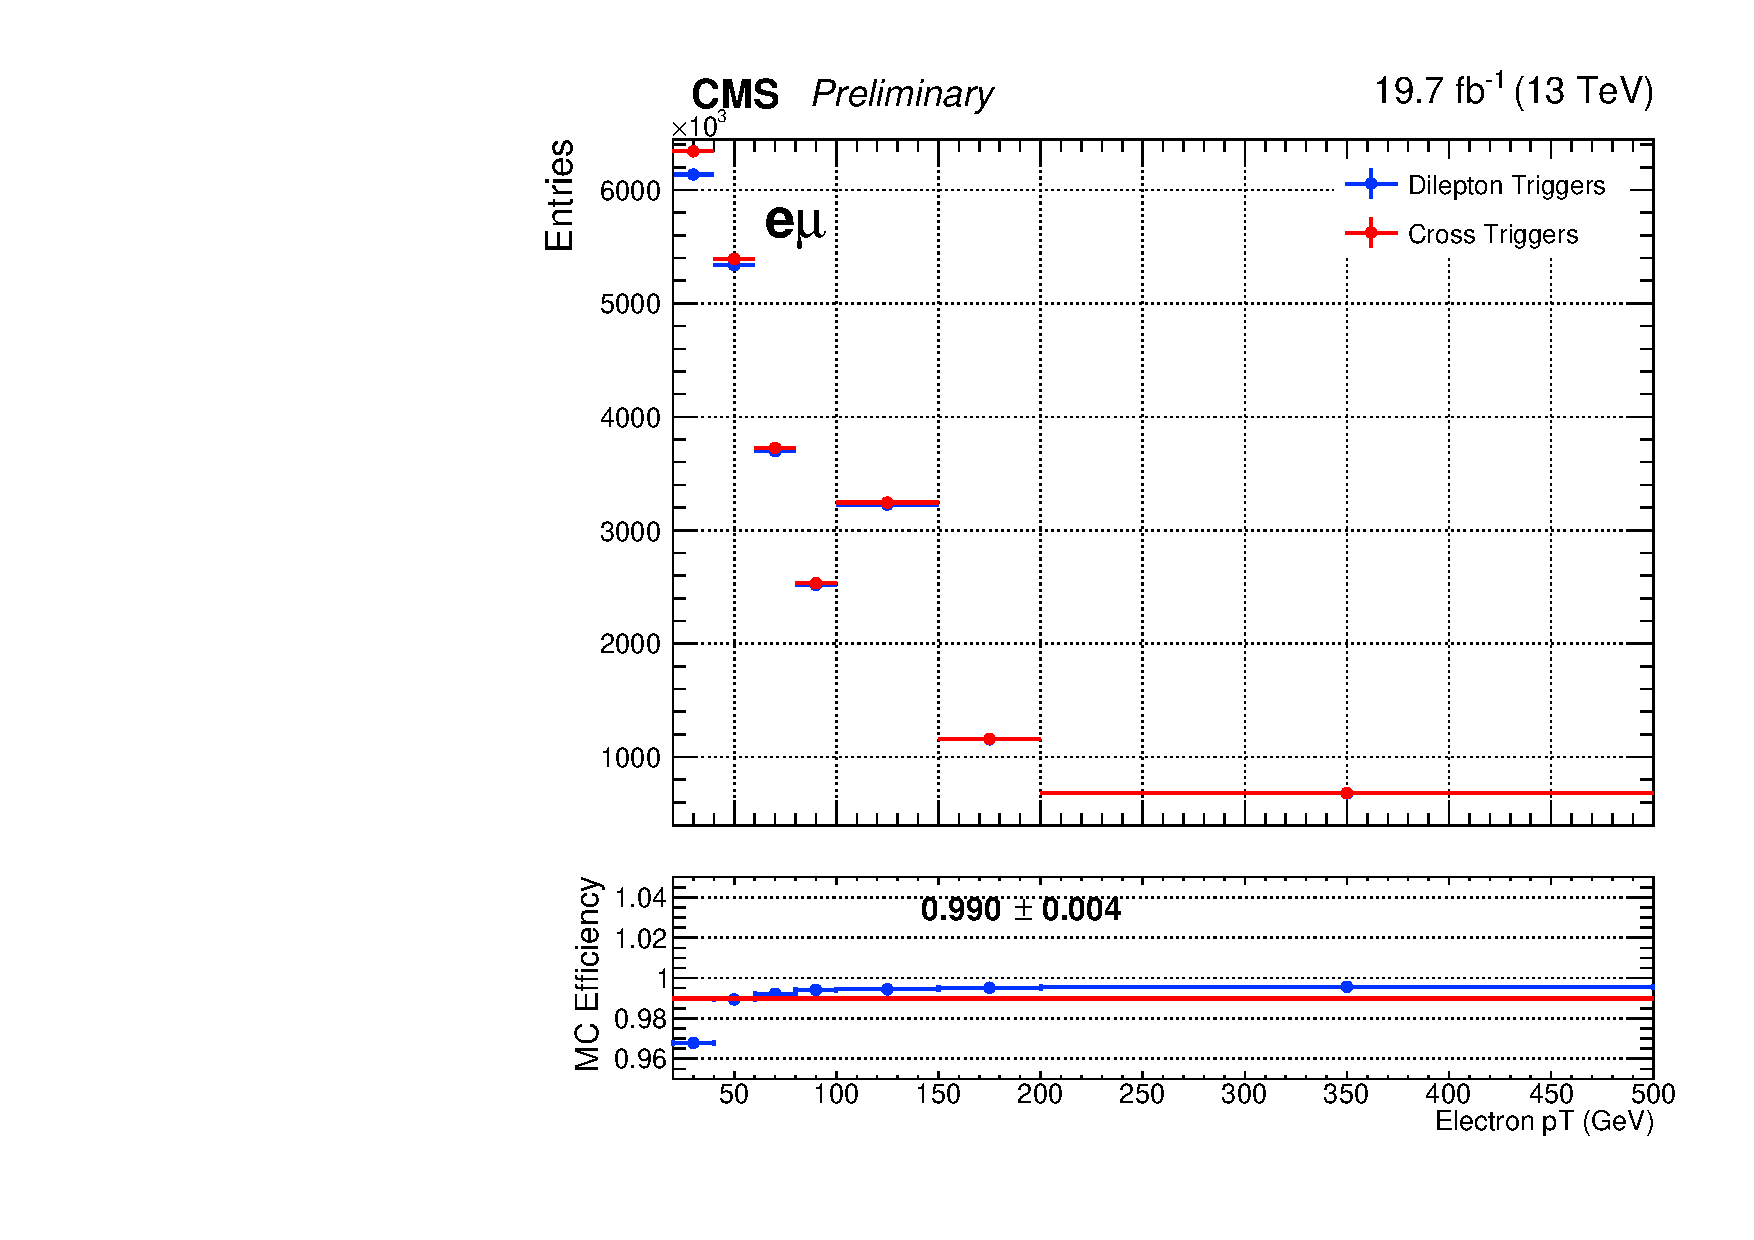
\includegraphics[width=0.32\textwidth]{fig_2016preVFP_TrigSF/g_lepApt_emu_MC.pdf}
      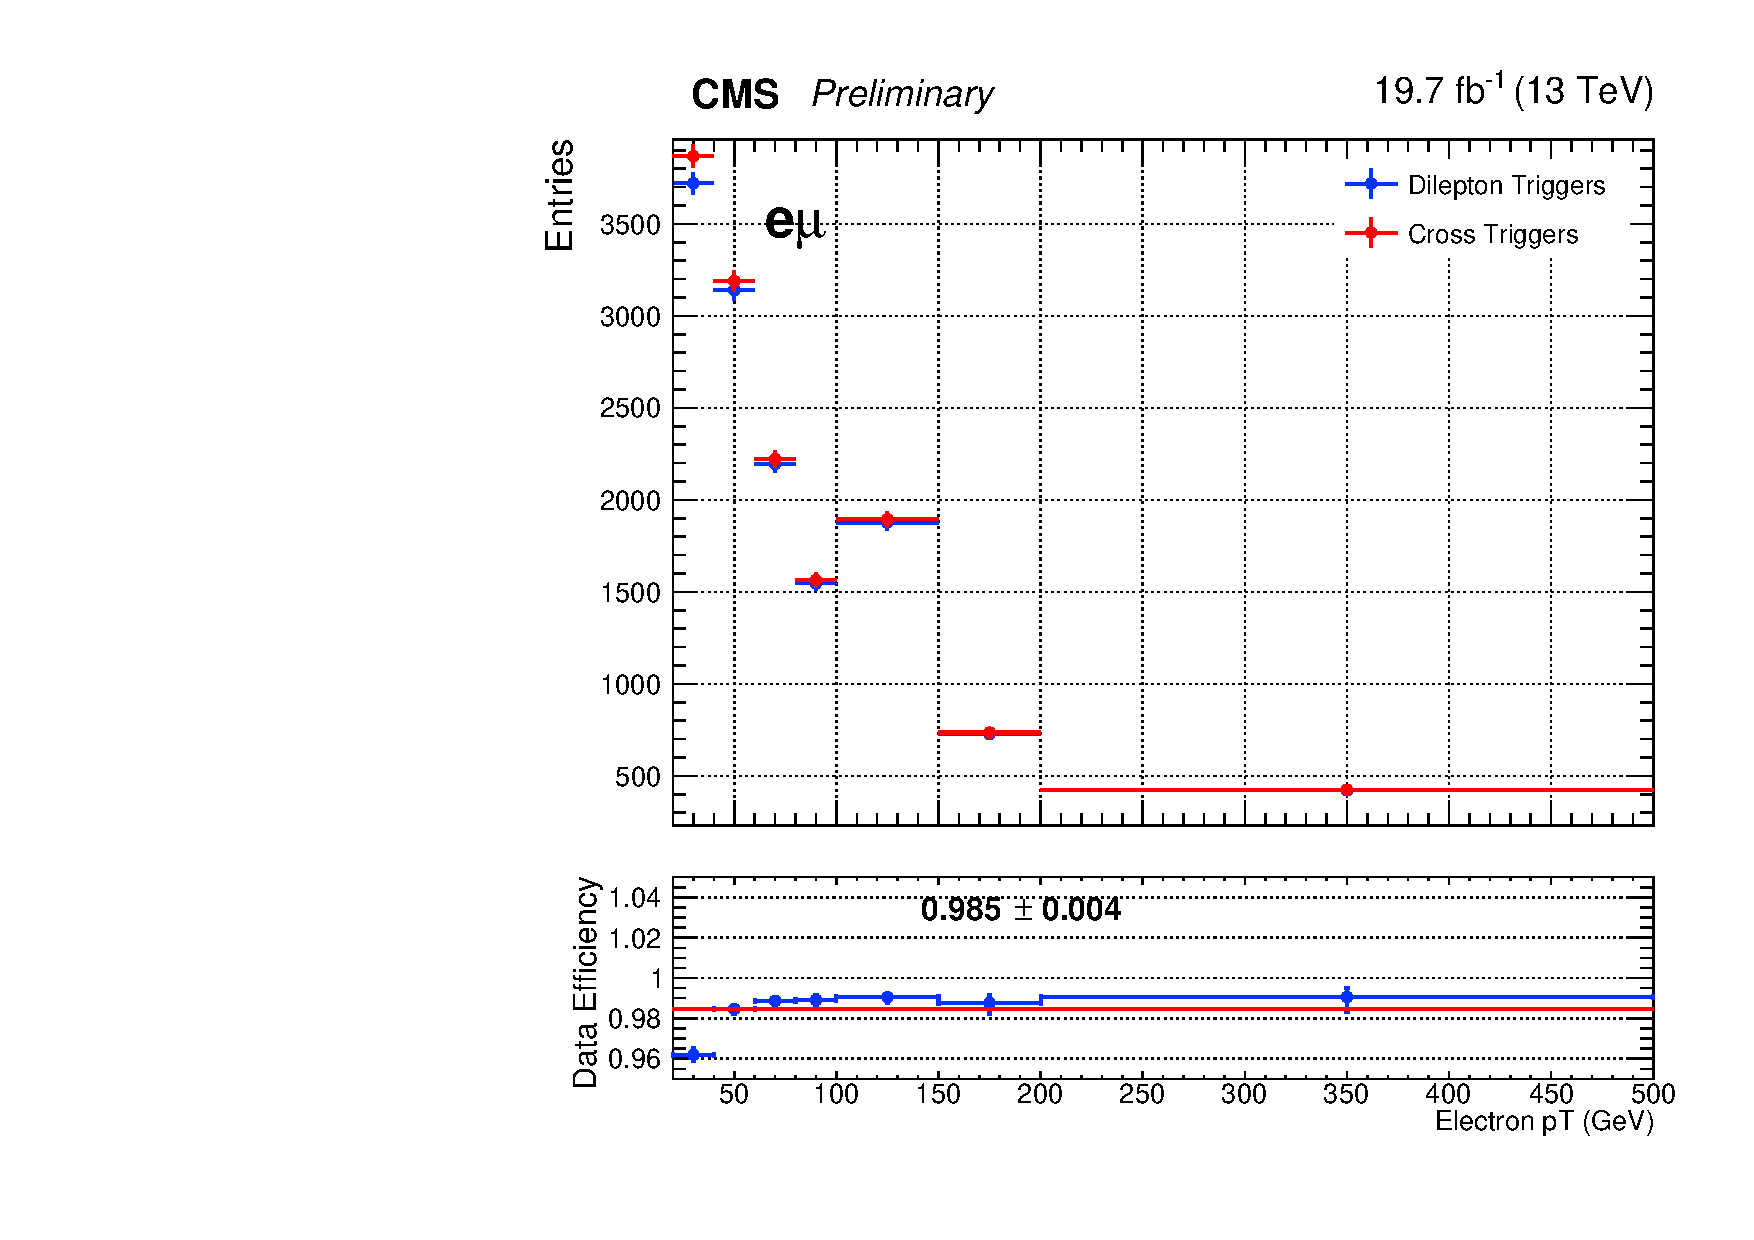
\includegraphics[width=0.32\textwidth]{fig_2016preVFP_TrigSF/g_lepApt_emu_data.pdf}
      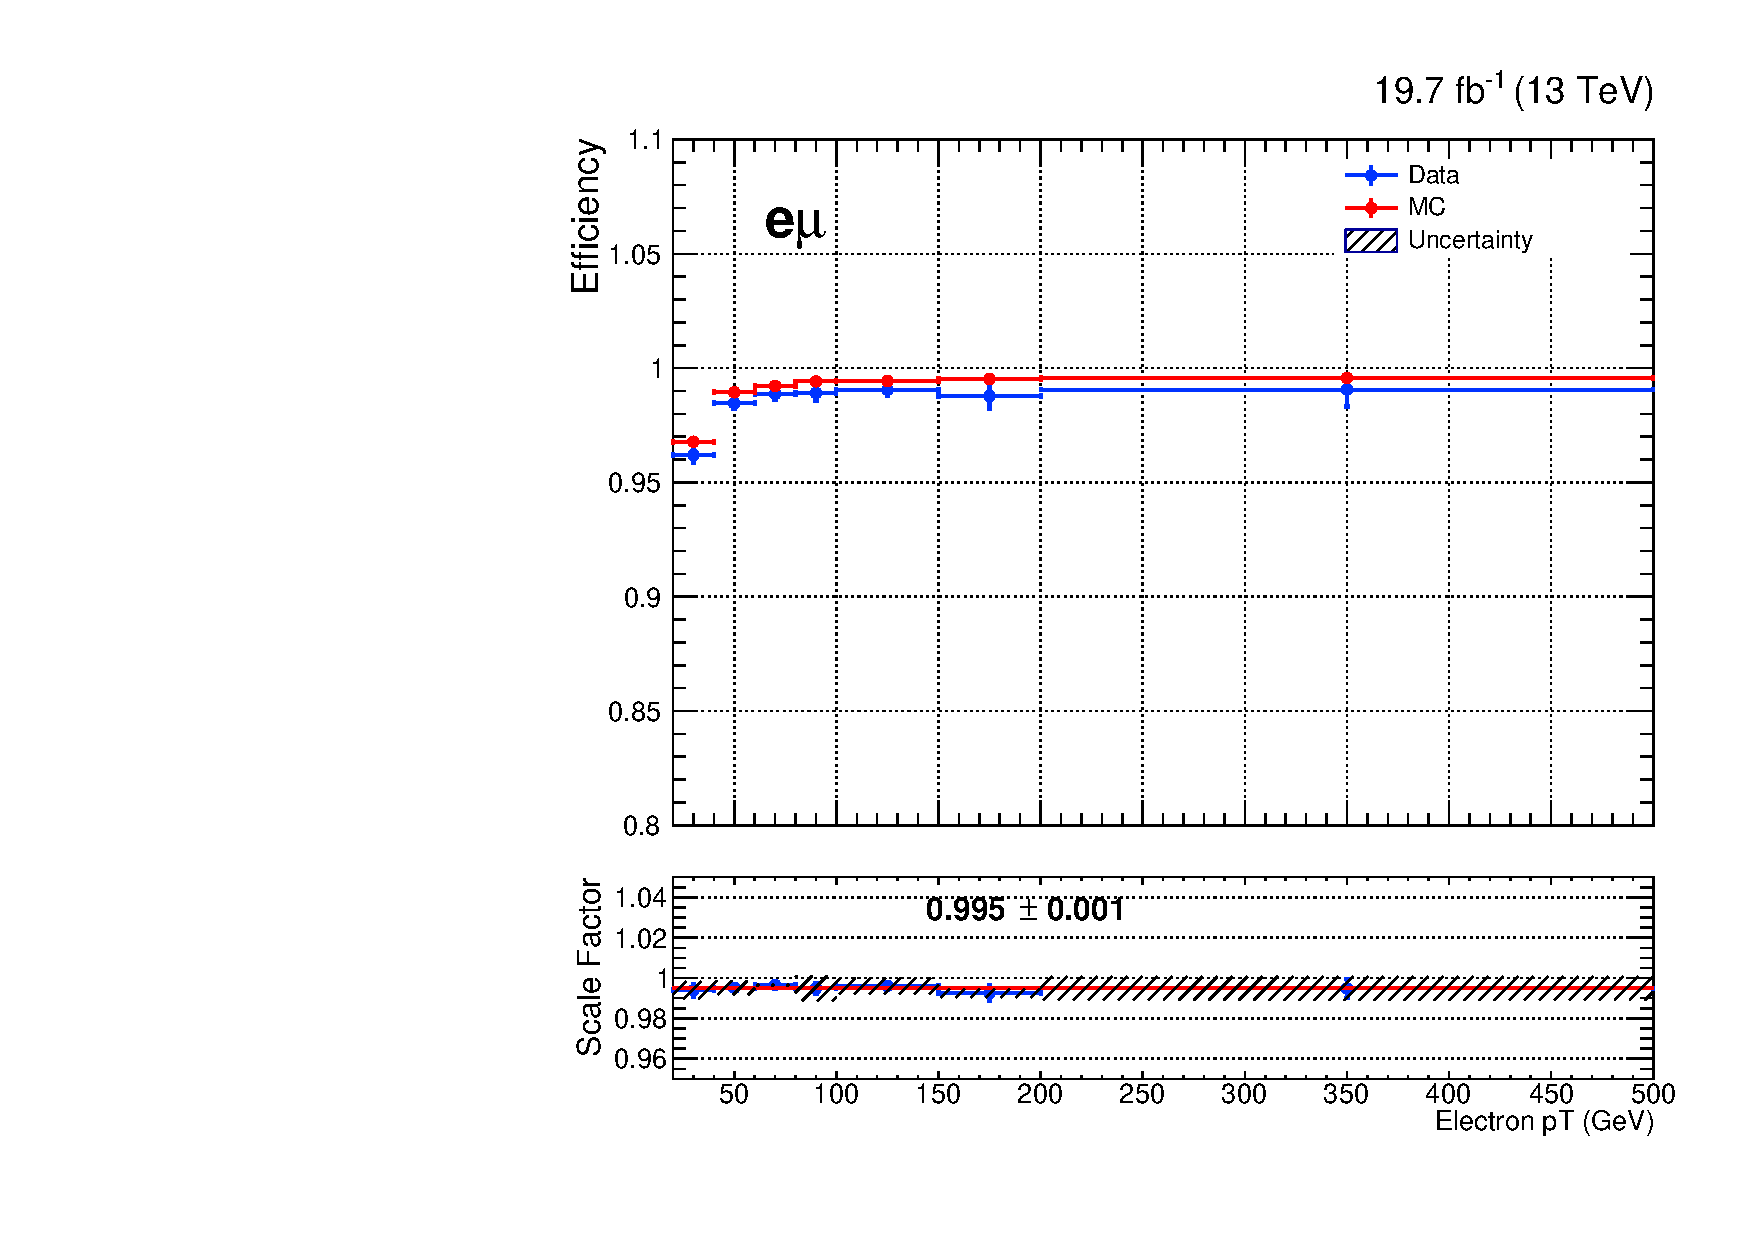
\includegraphics[width=0.32\textwidth]{fig_2016preVFP_TrigSF/g_emu_lepApt_FullSystUncBand.pdf}\\
      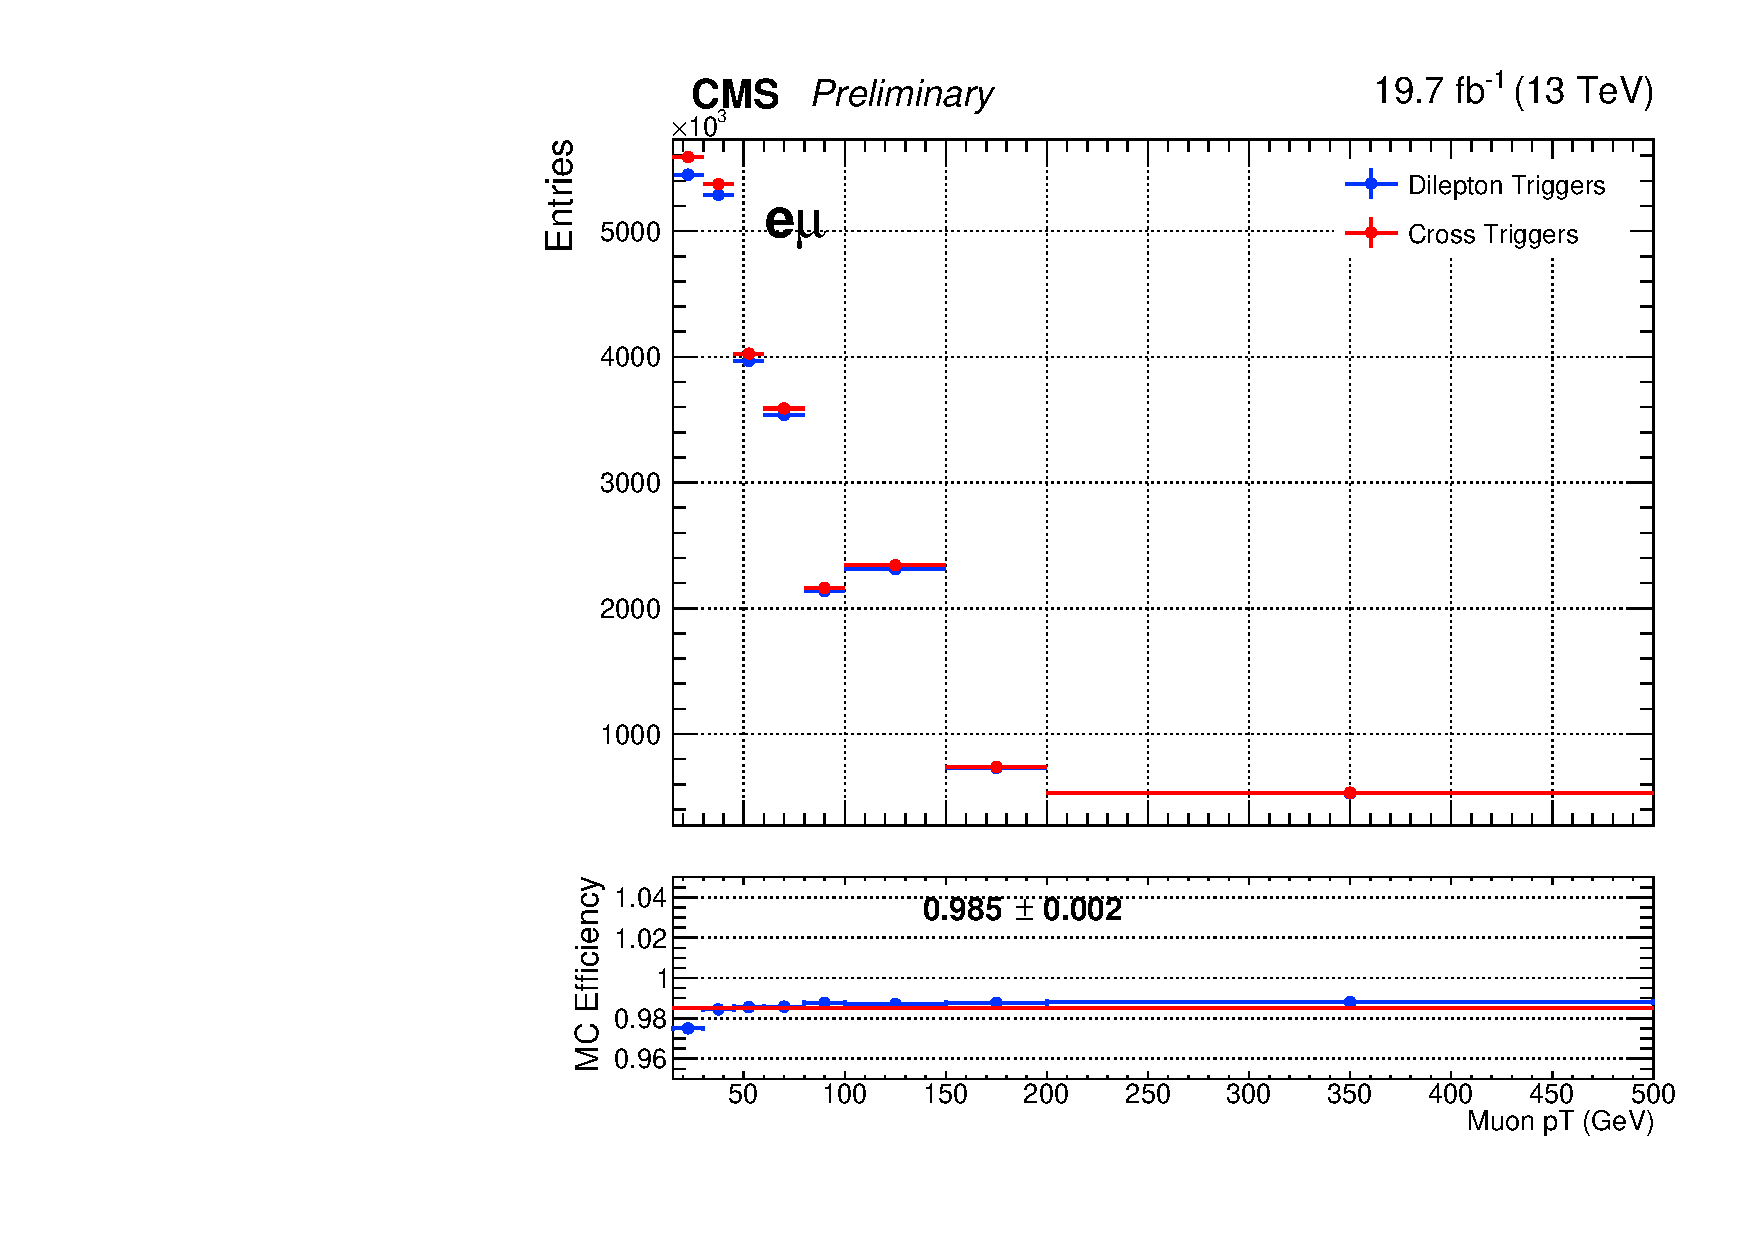
\includegraphics[width=0.32\textwidth]{fig_2016preVFP_TrigSF/g_lepBpt_emu_MC.pdf}
      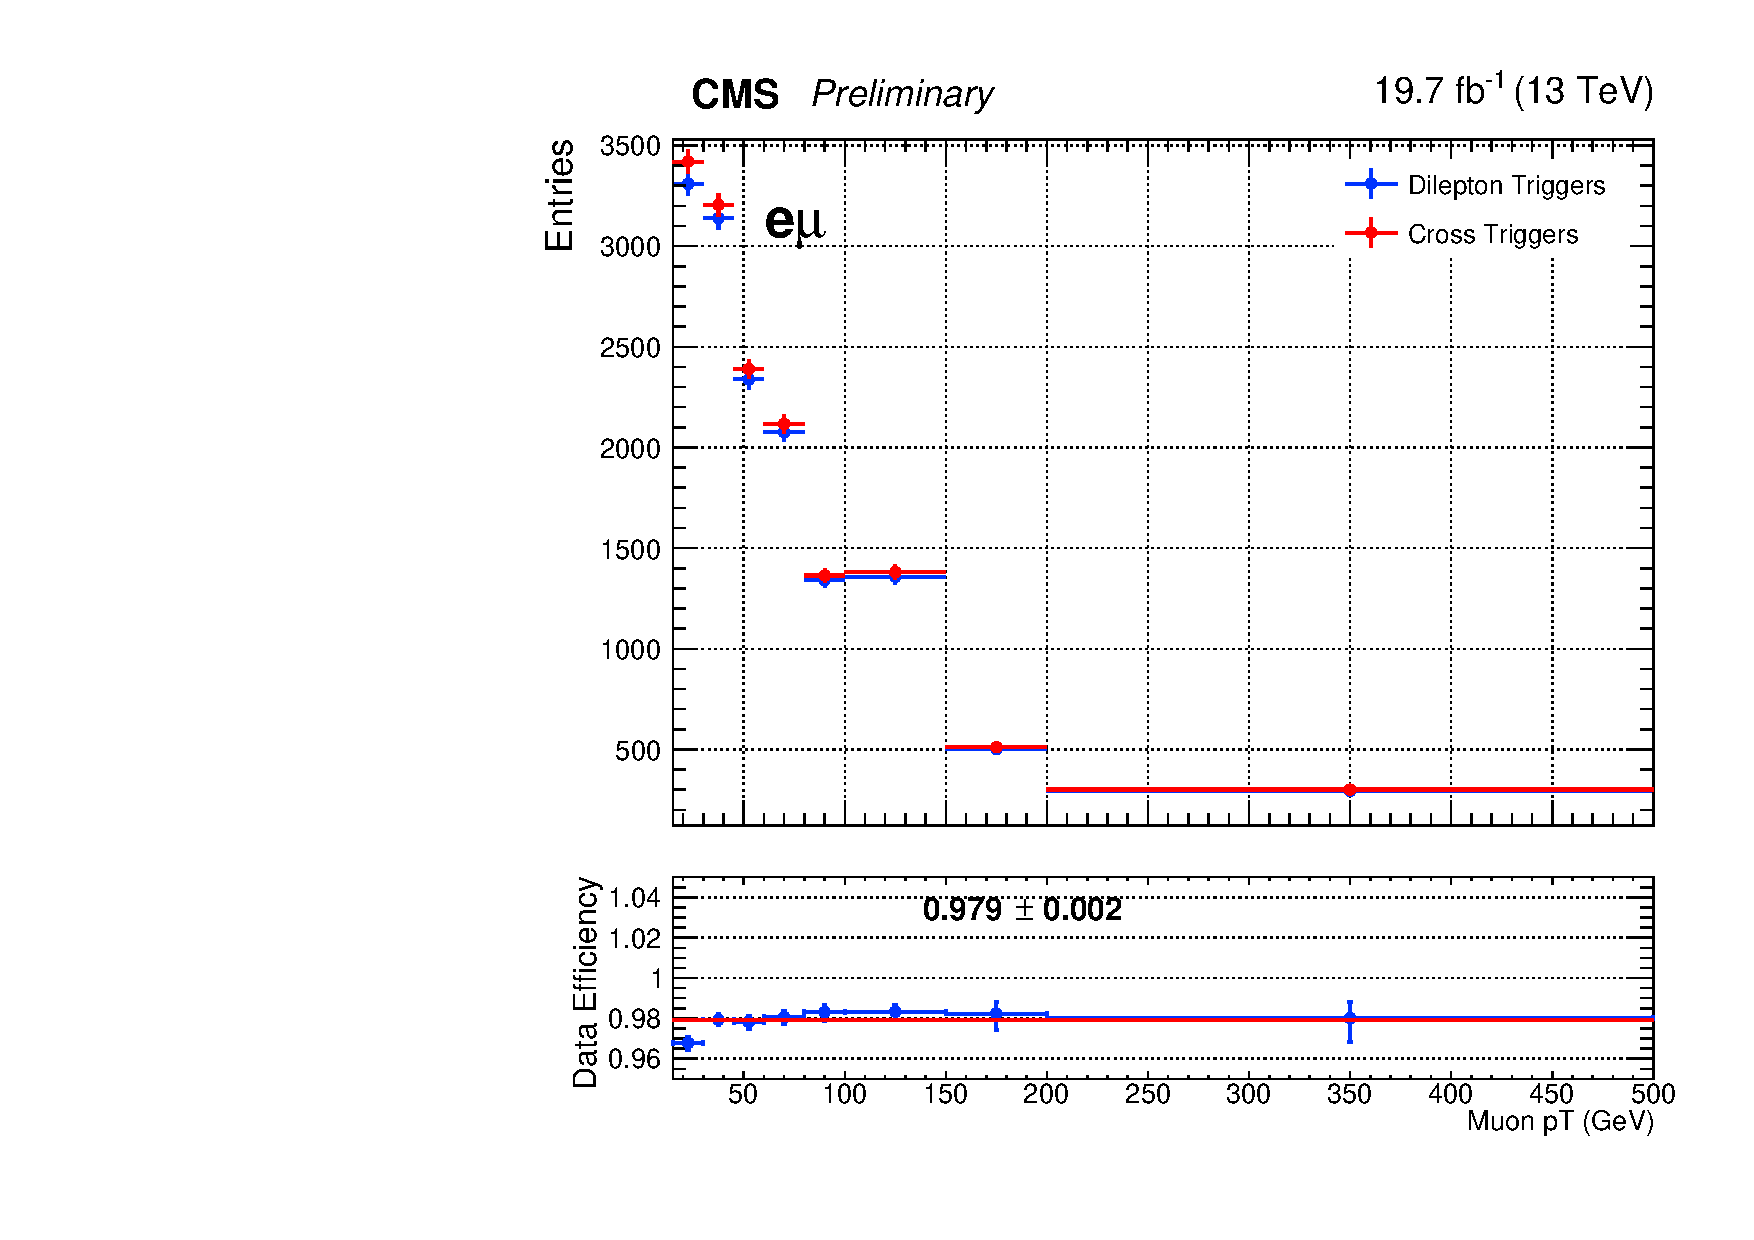
\includegraphics[width=0.32\textwidth]{fig_2016preVFP_TrigSF/g_lepBpt_emu_data.pdf}
      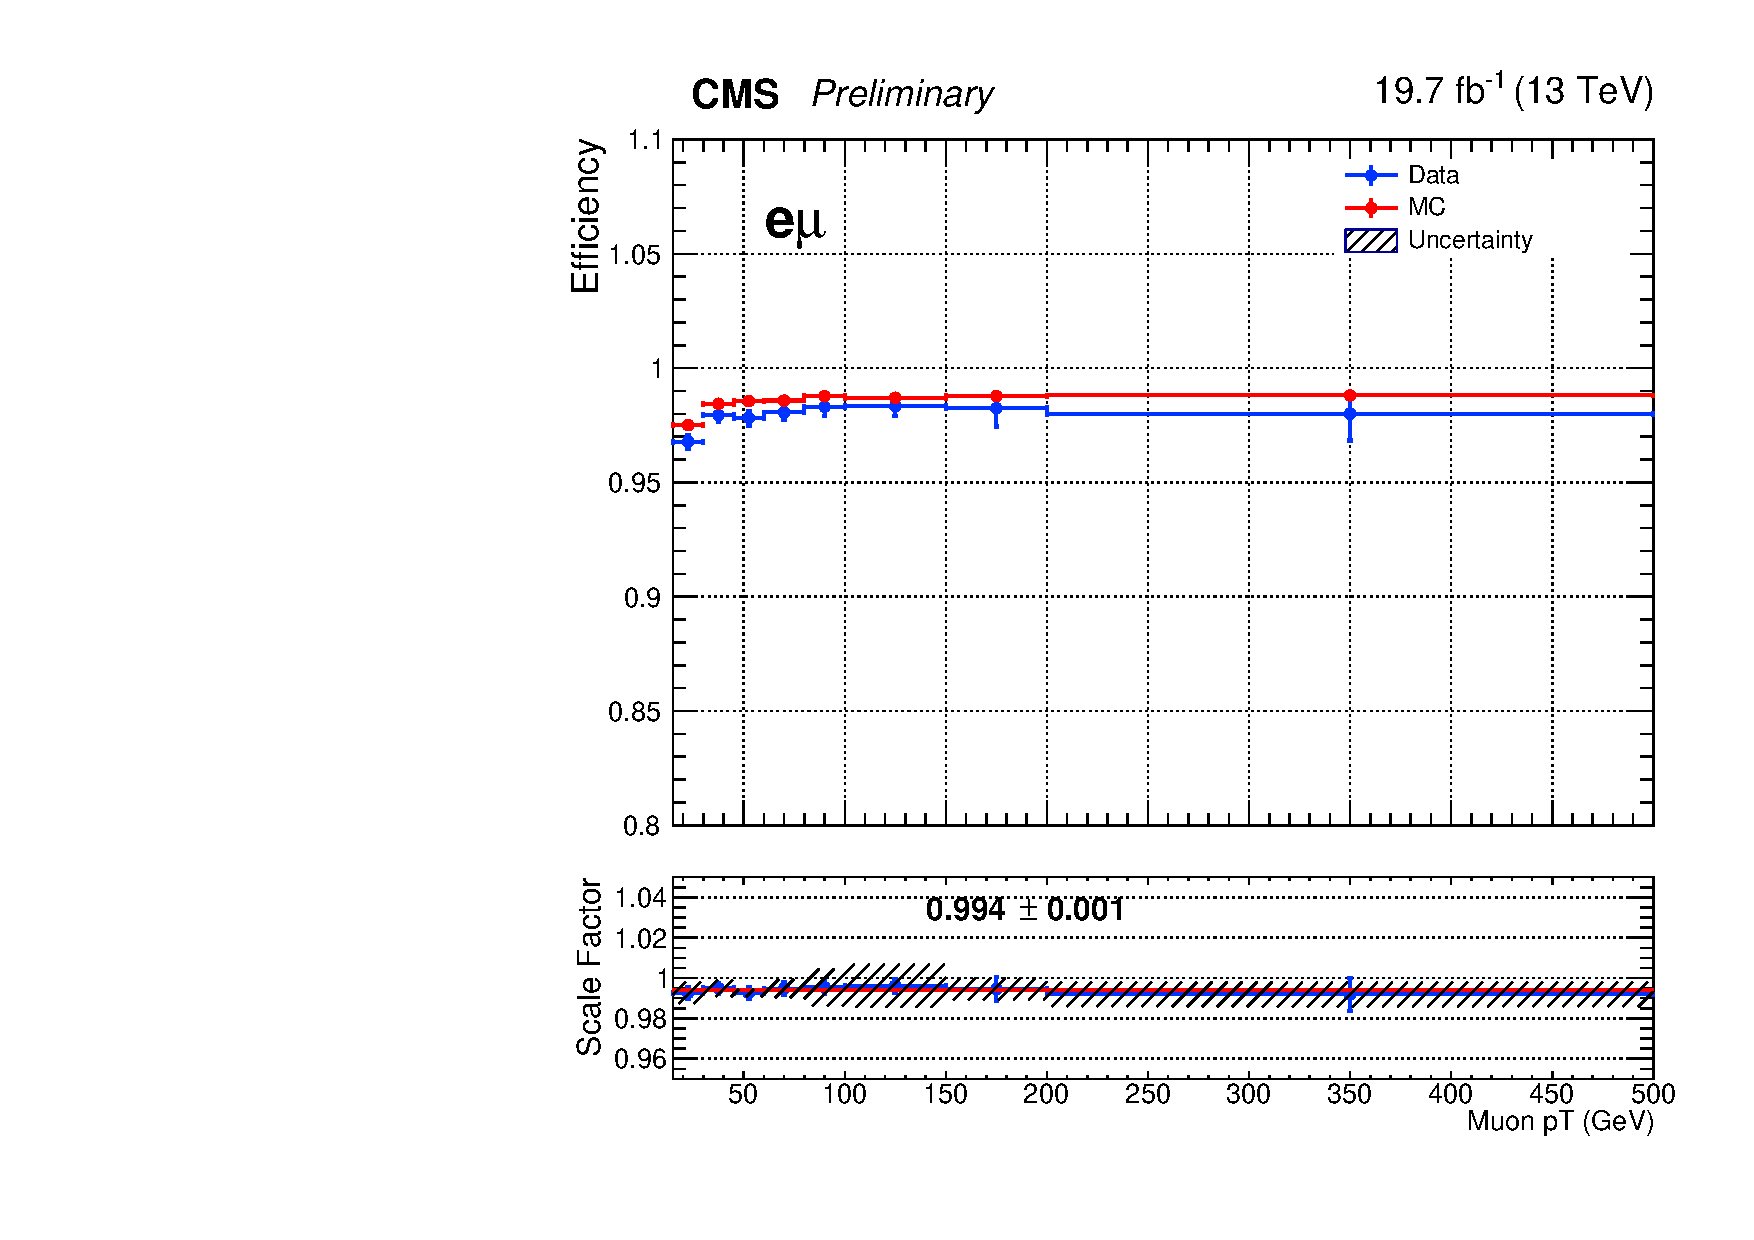
\includegraphics[width=0.32\textwidth]{fig_2016preVFP_TrigSF/g_emu_lepBpt_FullSystUncBand.pdf}\\
    \end{tabular}
    \caption{Efficiencies and scale factors for the 2016preVFP data set in the $e\mu$ channel as a function of electron and muon \pT.
            The error bars indicate the statistical uncertainty, and the shaded band corresponds to the systematic uncertainty.
            }
    \label{TrigSF_2016preVFP_1}
  \end{center}
\end{figure}

\begin{figure}[h]
  \begin{center}
    \begin{tabular}{ccc}
      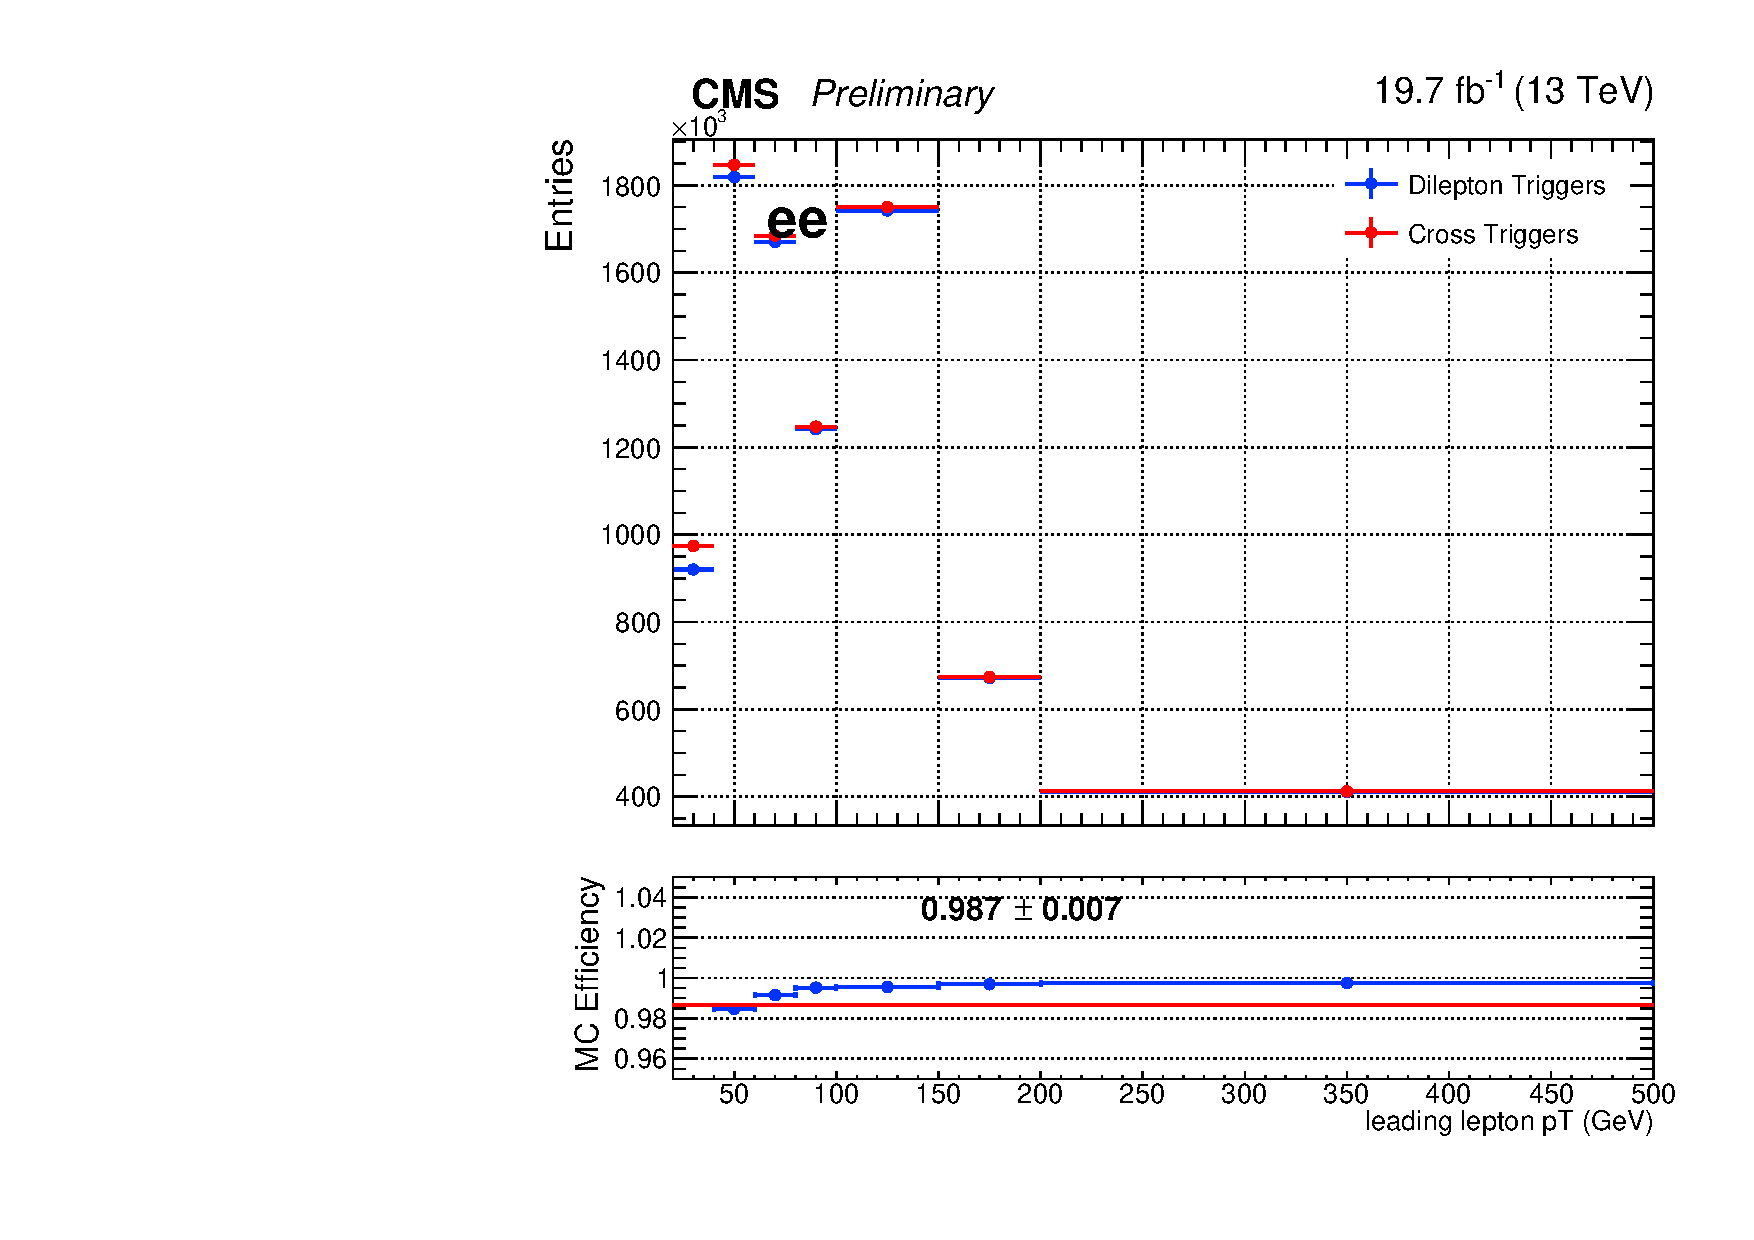
\includegraphics[width=0.32\textwidth]{fig_2016preVFP_TrigSF/g_lepApt_ee_MC.pdf}
      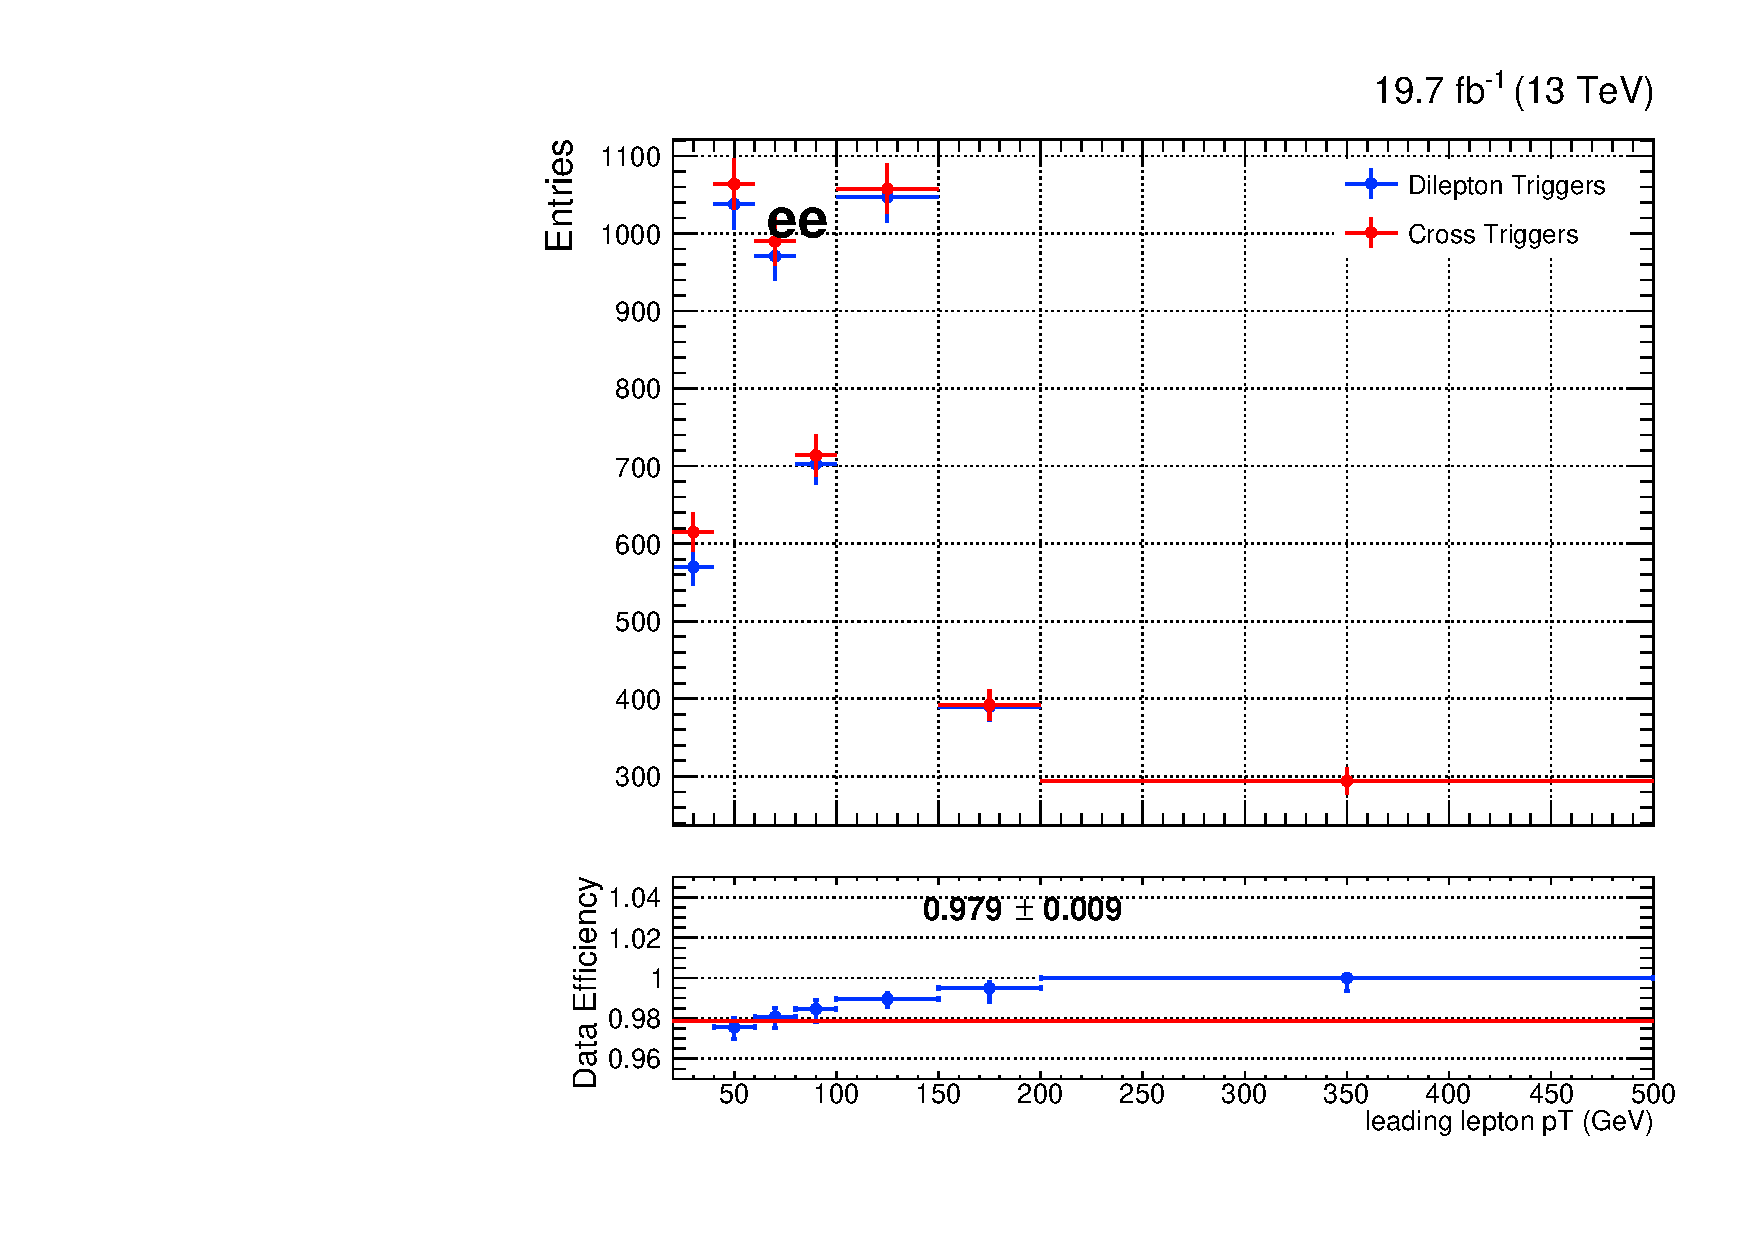
\includegraphics[width=0.32\textwidth]{fig_2016preVFP_TrigSF/g_lepApt_ee_data.pdf}
      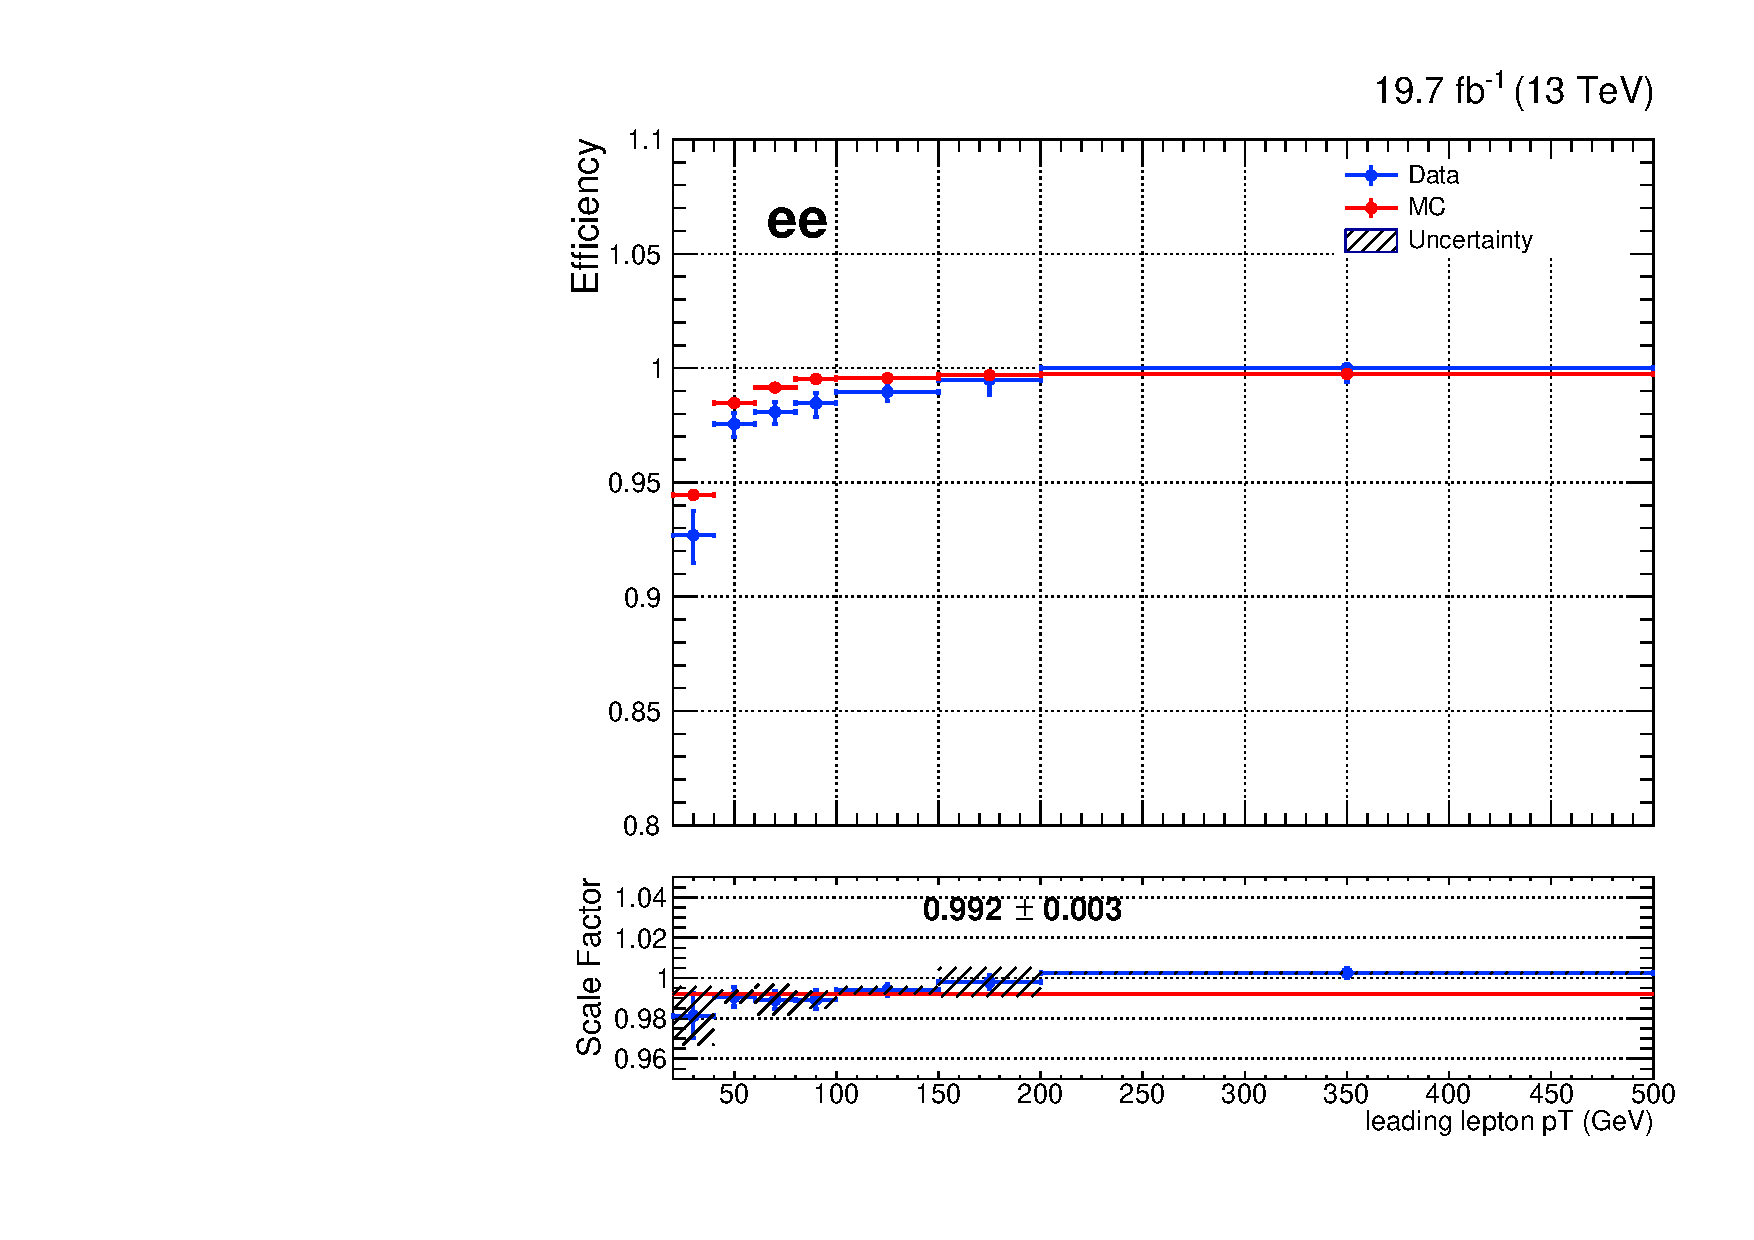
\includegraphics[width=0.32\textwidth]{fig_2016preVFP_TrigSF/g_ee_lepApt_FullSystUncBand.pdf}\\
      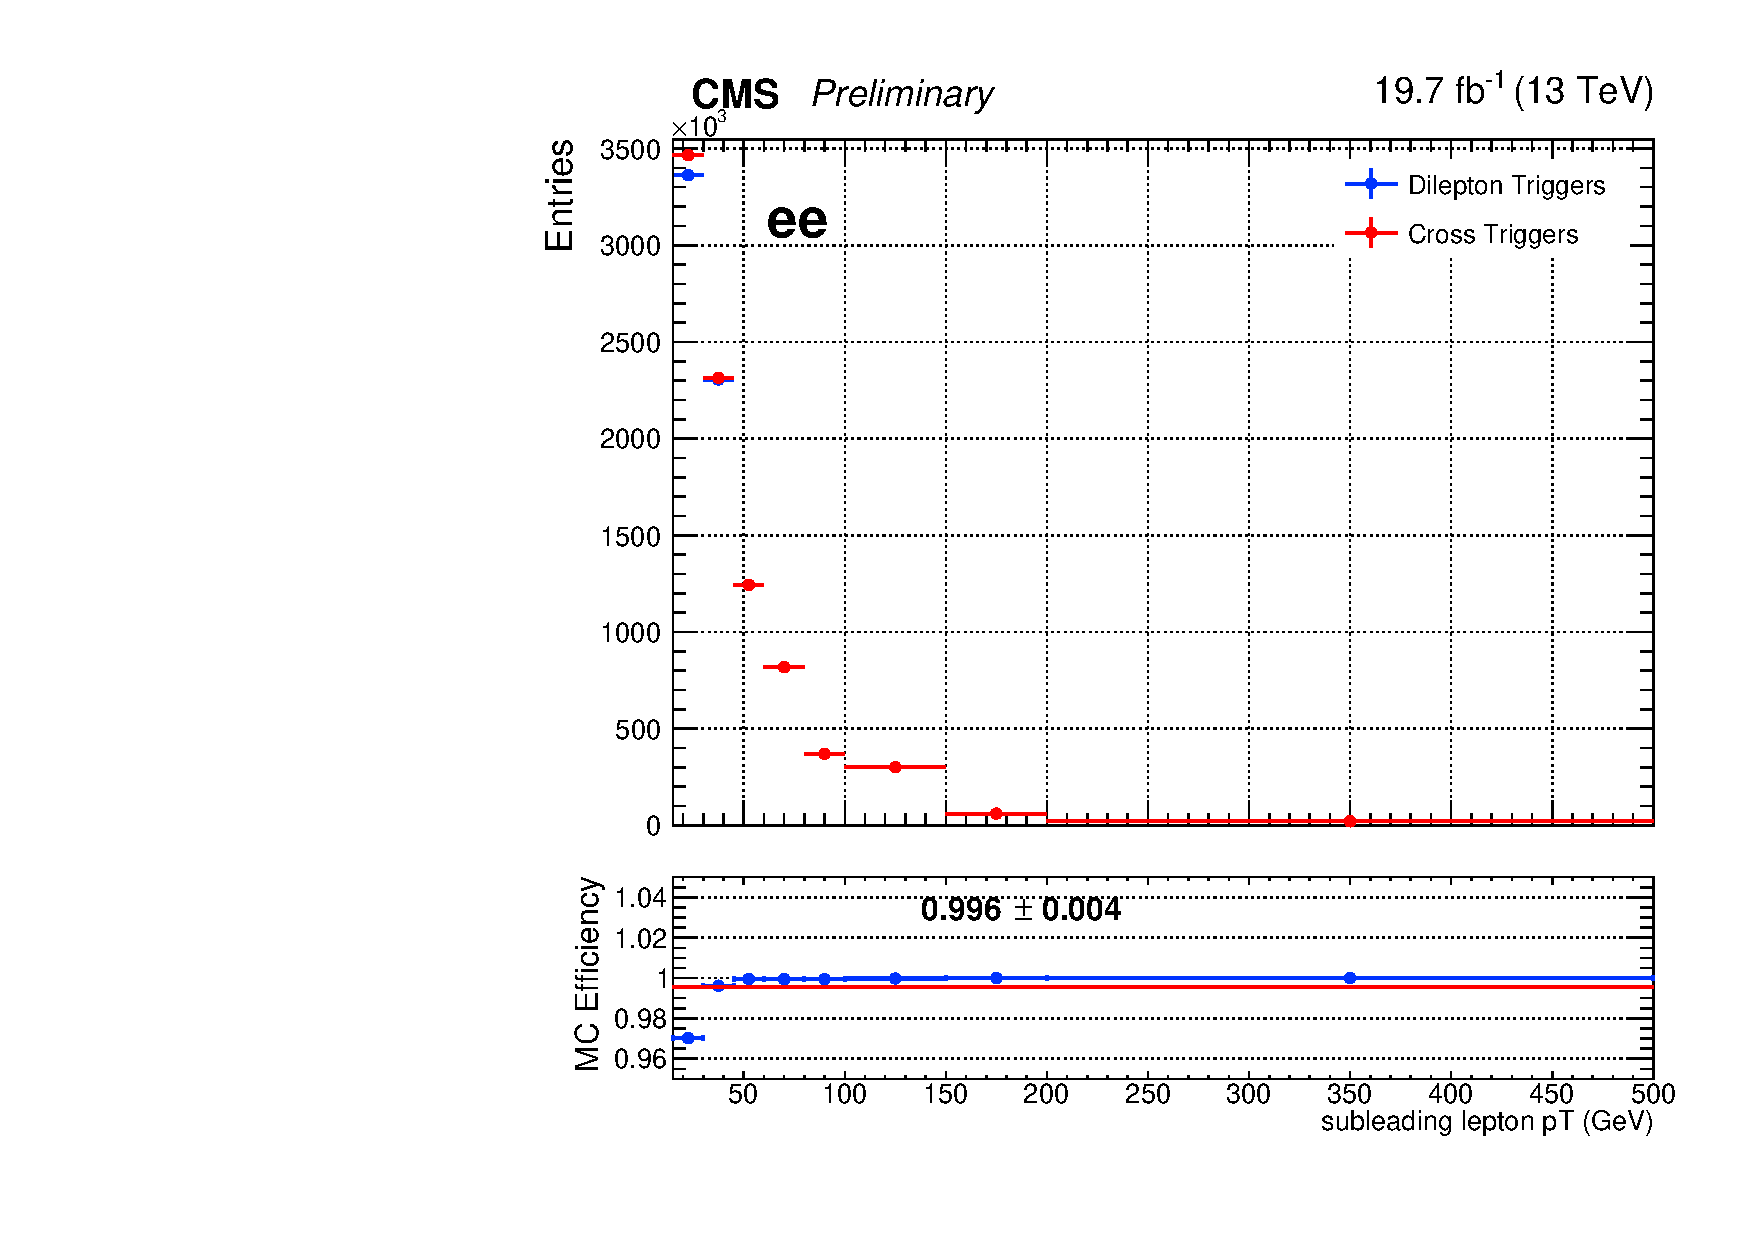
\includegraphics[width=0.32\textwidth]{fig_2016preVFP_TrigSF/g_lepBpt_ee_MC.pdf}
      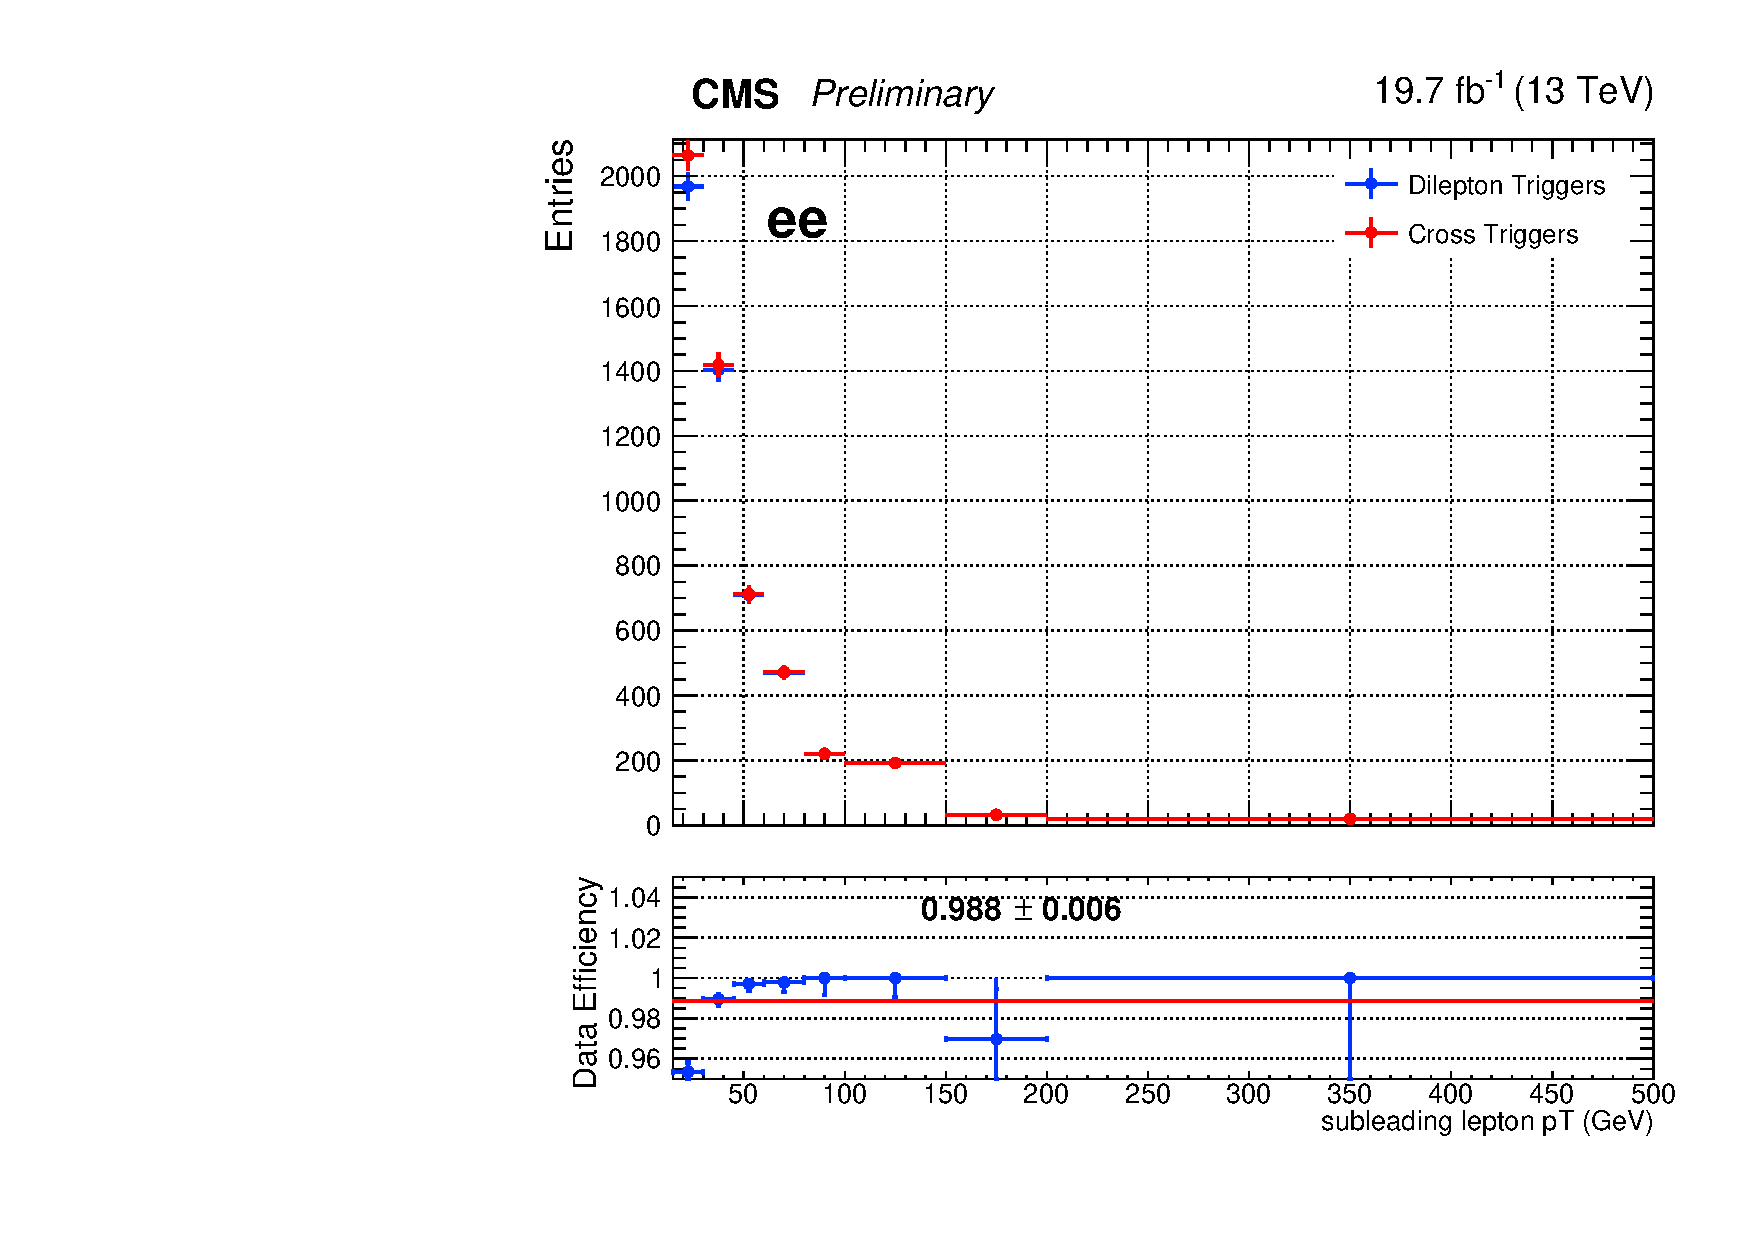
\includegraphics[width=0.32\textwidth]{fig_2016preVFP_TrigSF/g_lepBpt_ee_data.pdf}
      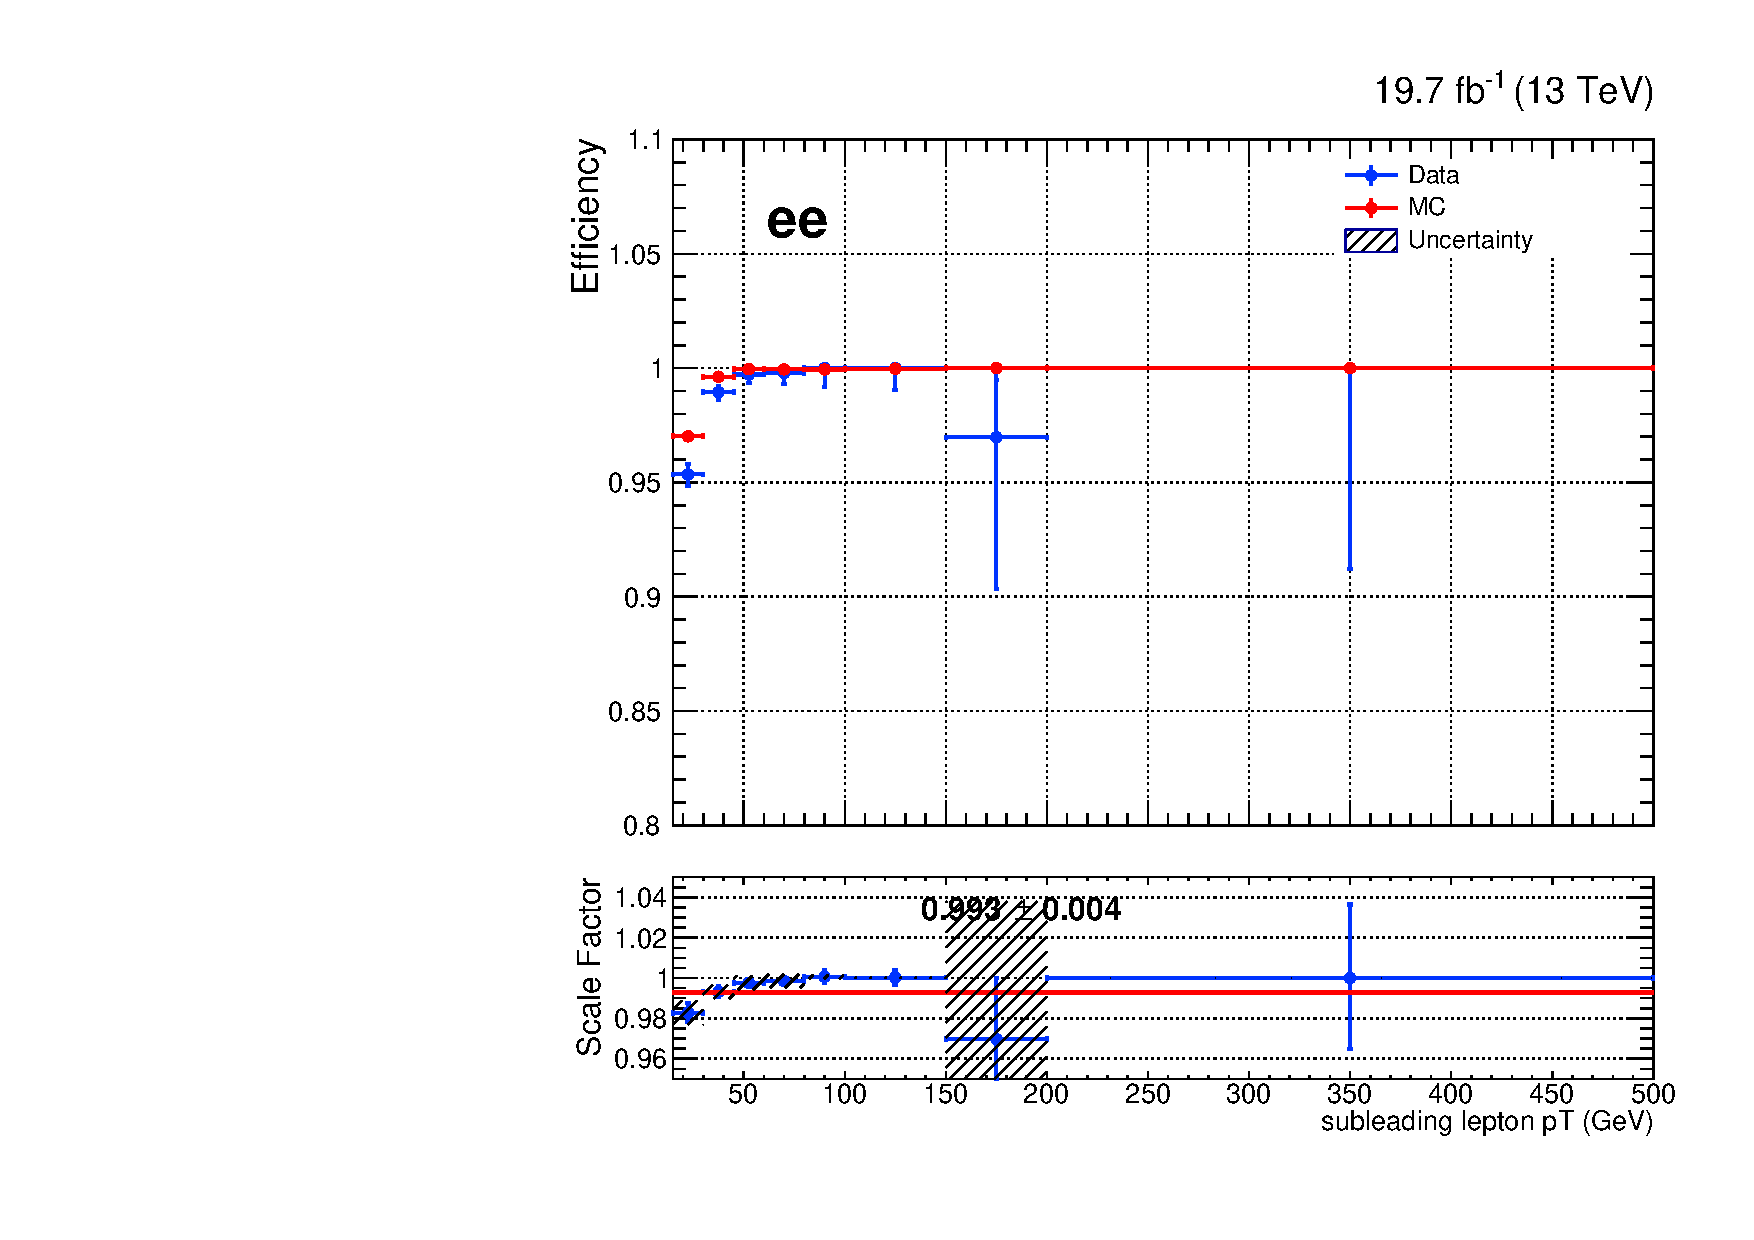
\includegraphics[width=0.32\textwidth]{fig_2016preVFP_TrigSF/g_ee_lepBpt_FullSystUncBand.pdf}\\
    \end{tabular}
    \caption{Efficiencies and scale factors for the 2016preVFP data set in the $ee$ channel as a function of leading and sub-leading lepton \pT.
            The error bars indicate the statistical uncertainty, and the shaded band corresponds to the systematic uncertainty.
            }
    \label{TrigSF_2016preVFP_2}
  \end{center}
\end{figure}

\begin{figure}[h]
  \begin{center}
    \begin{tabular}{ccc}
      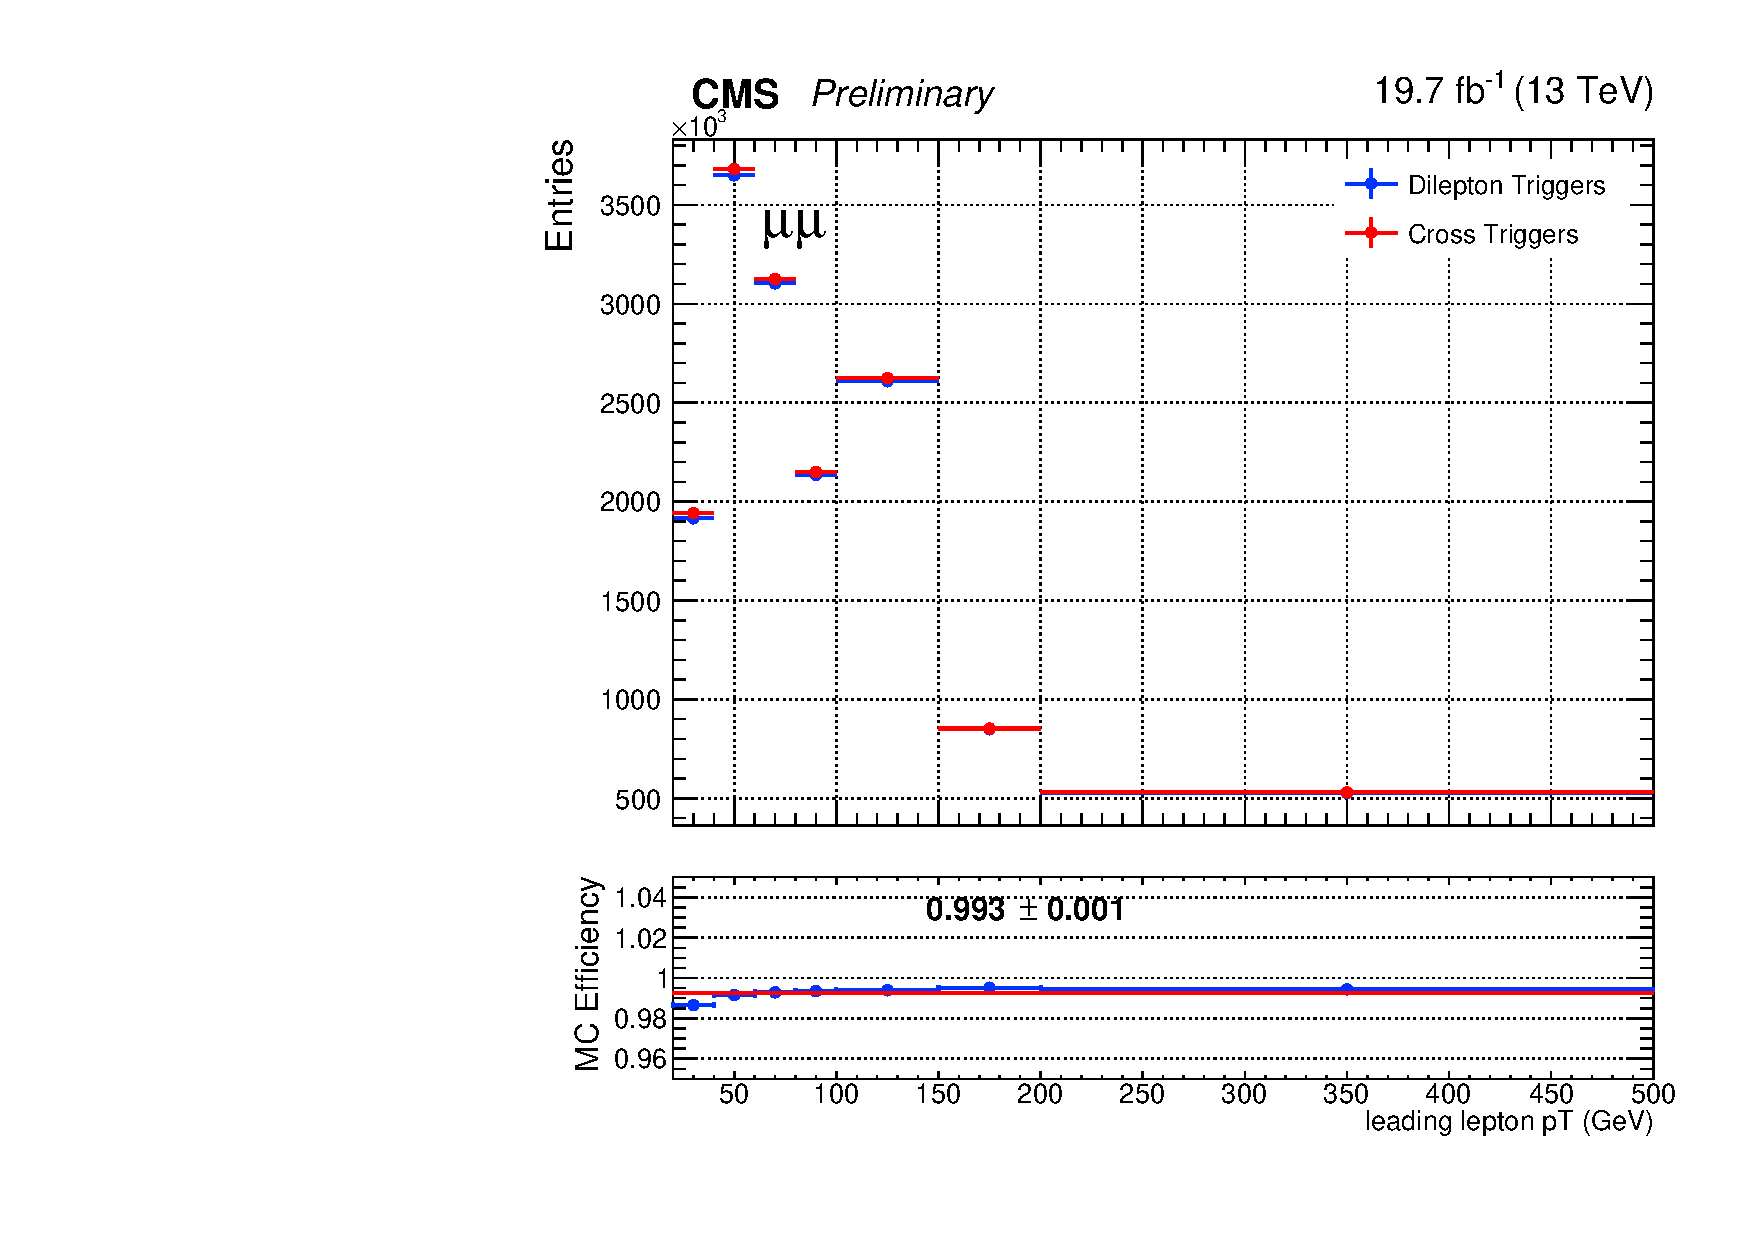
\includegraphics[width=0.32\textwidth]{fig_2016preVFP_TrigSF/g_lepApt_mumu_MC.pdf}
      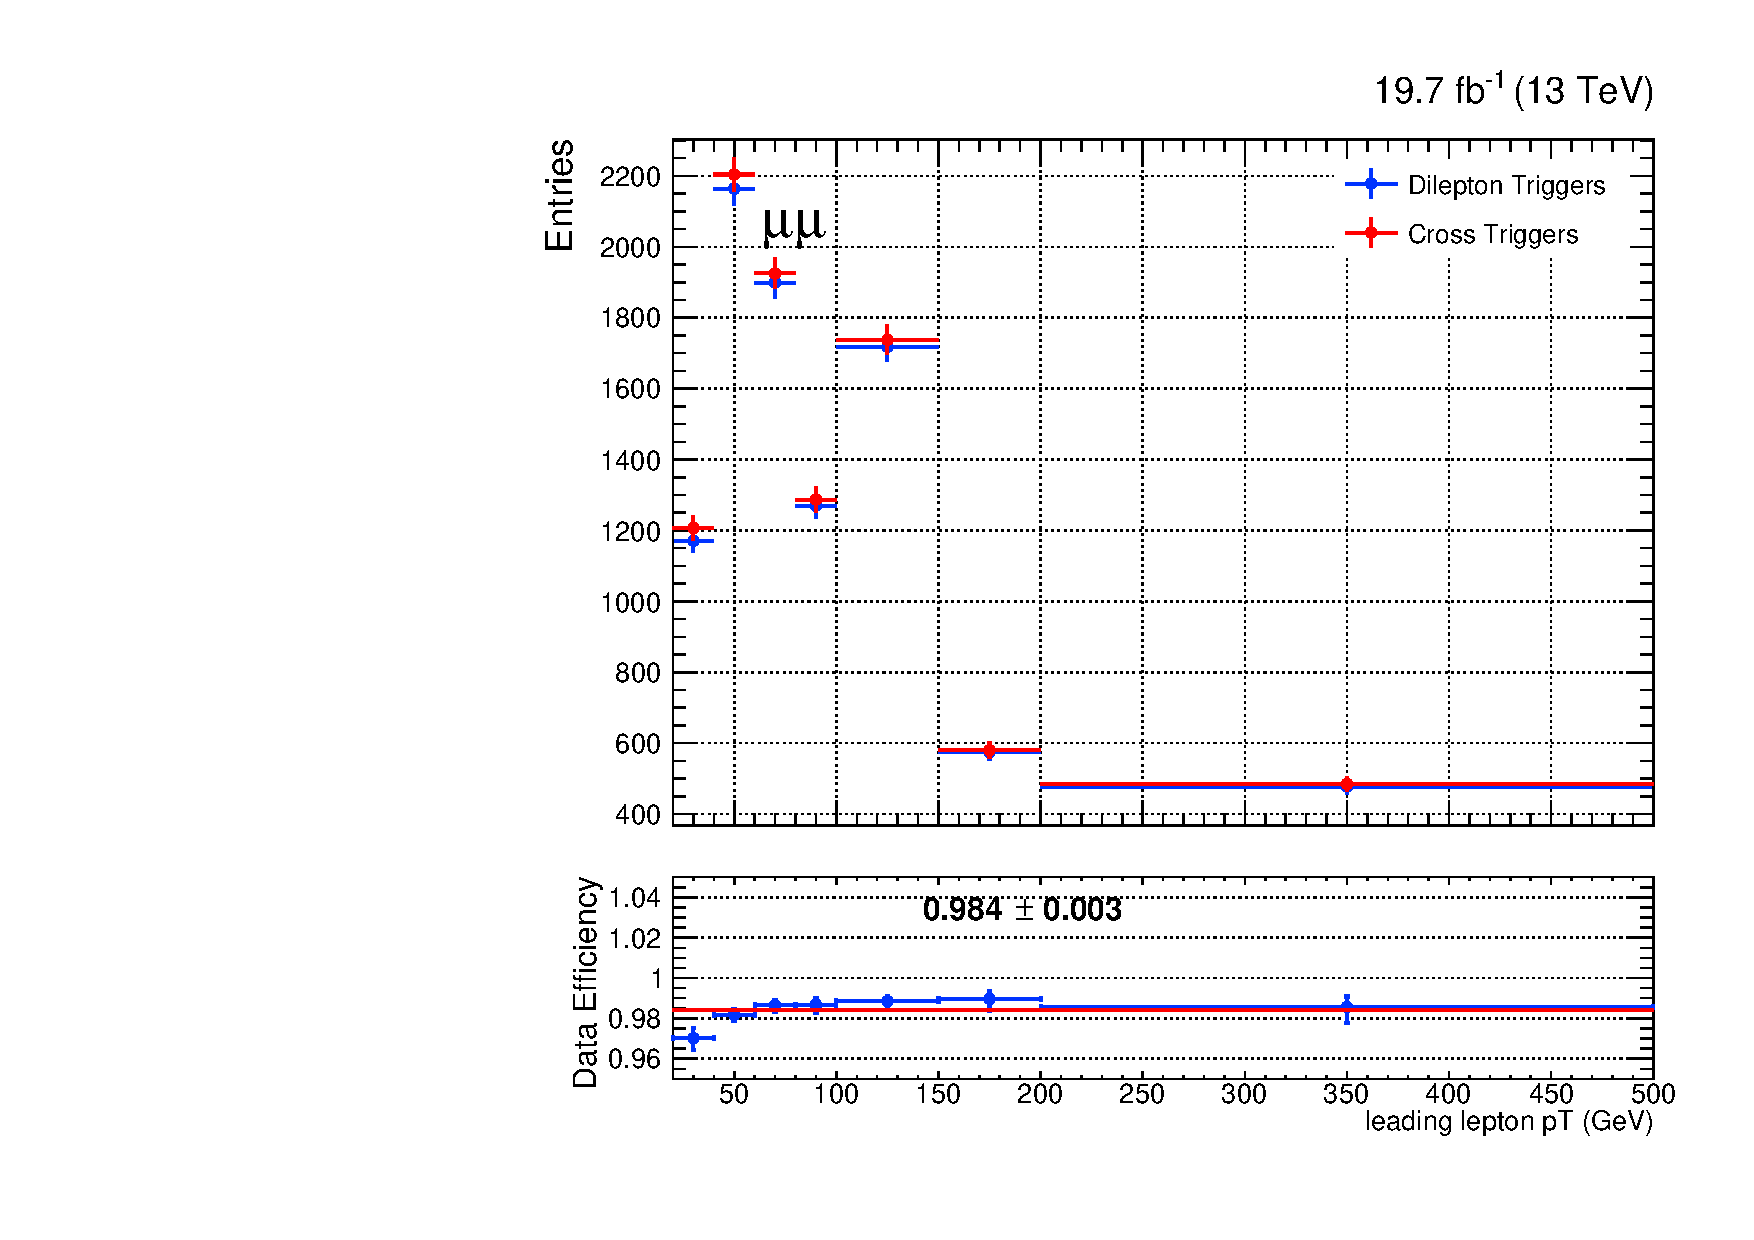
\includegraphics[width=0.32\textwidth]{fig_2016preVFP_TrigSF/g_lepApt_mumu_data.pdf}
      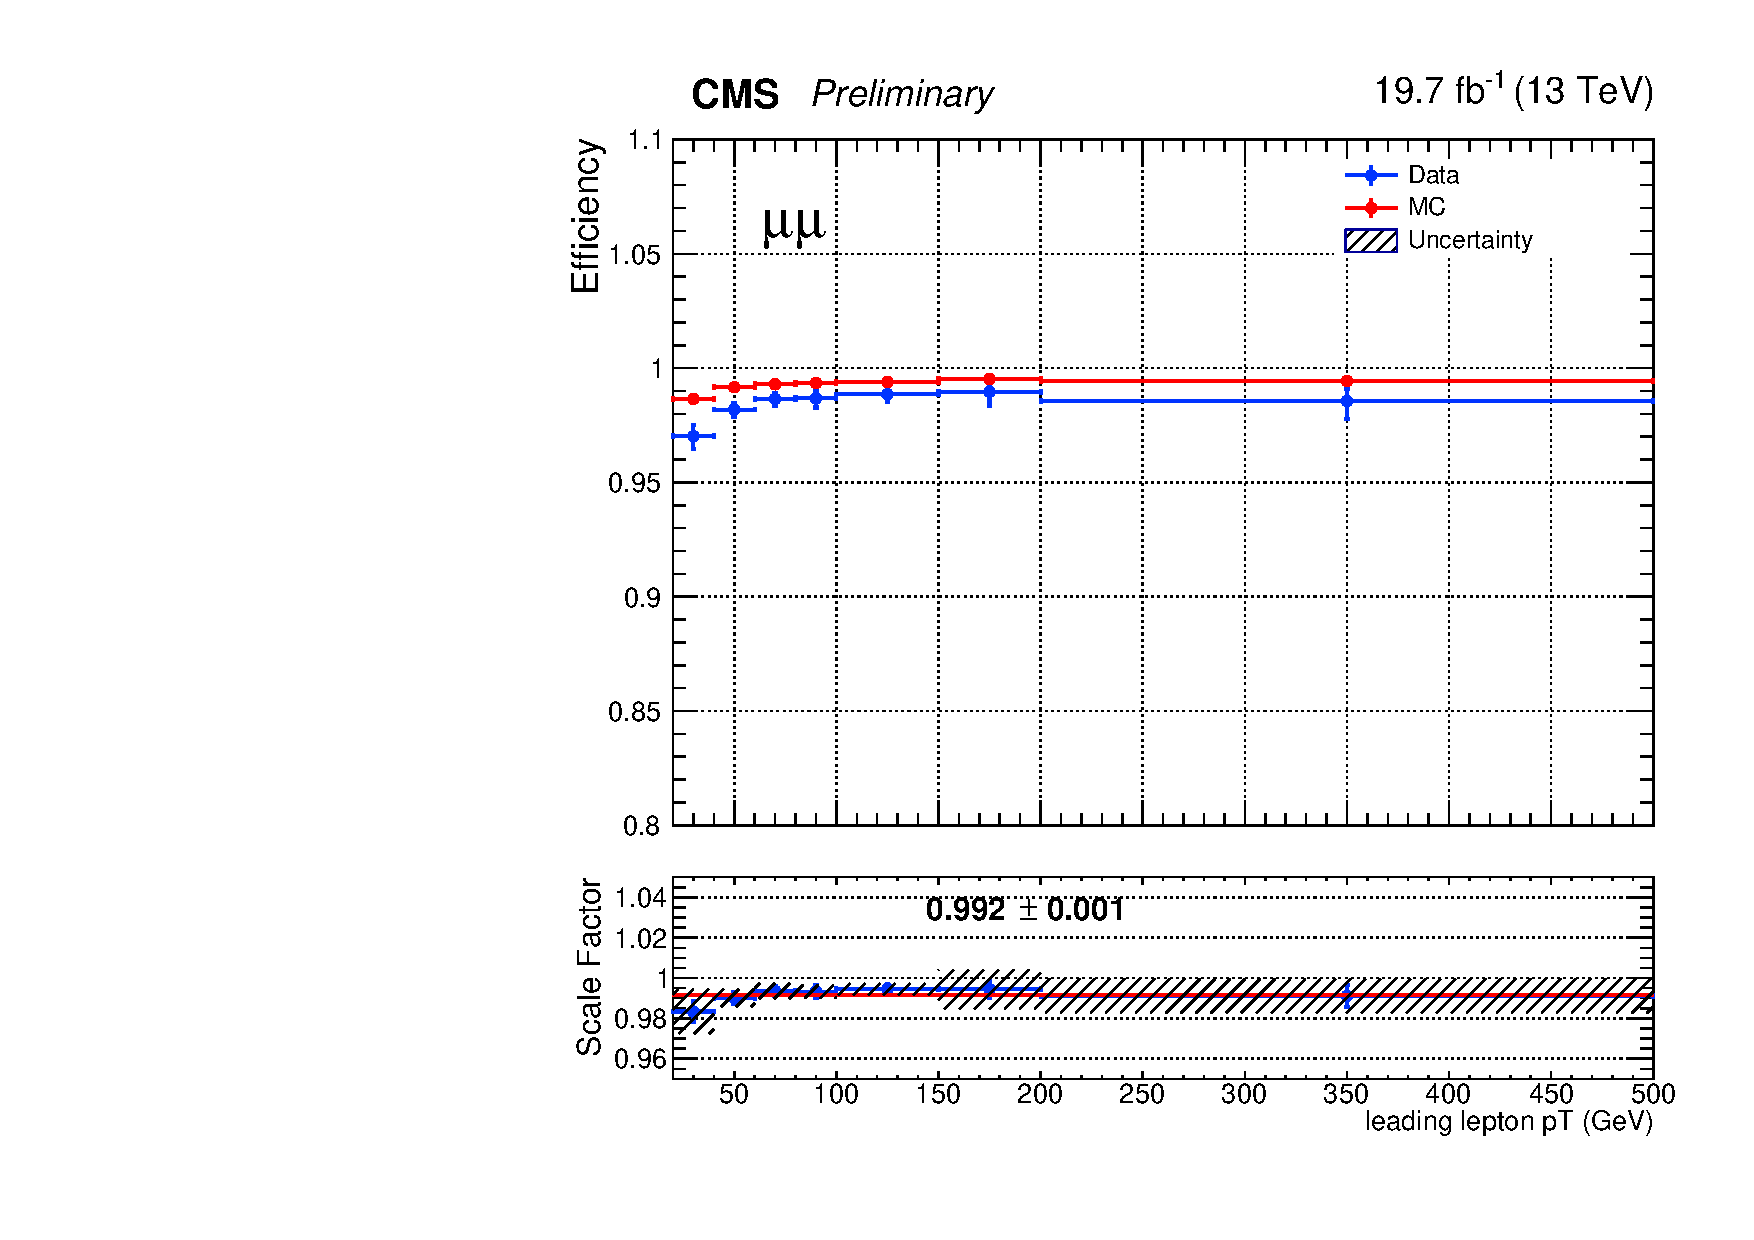
\includegraphics[width=0.32\textwidth]{fig_2016preVFP_TrigSF/g_mumu_lepApt_FullSystUncBand.pdf}\\
      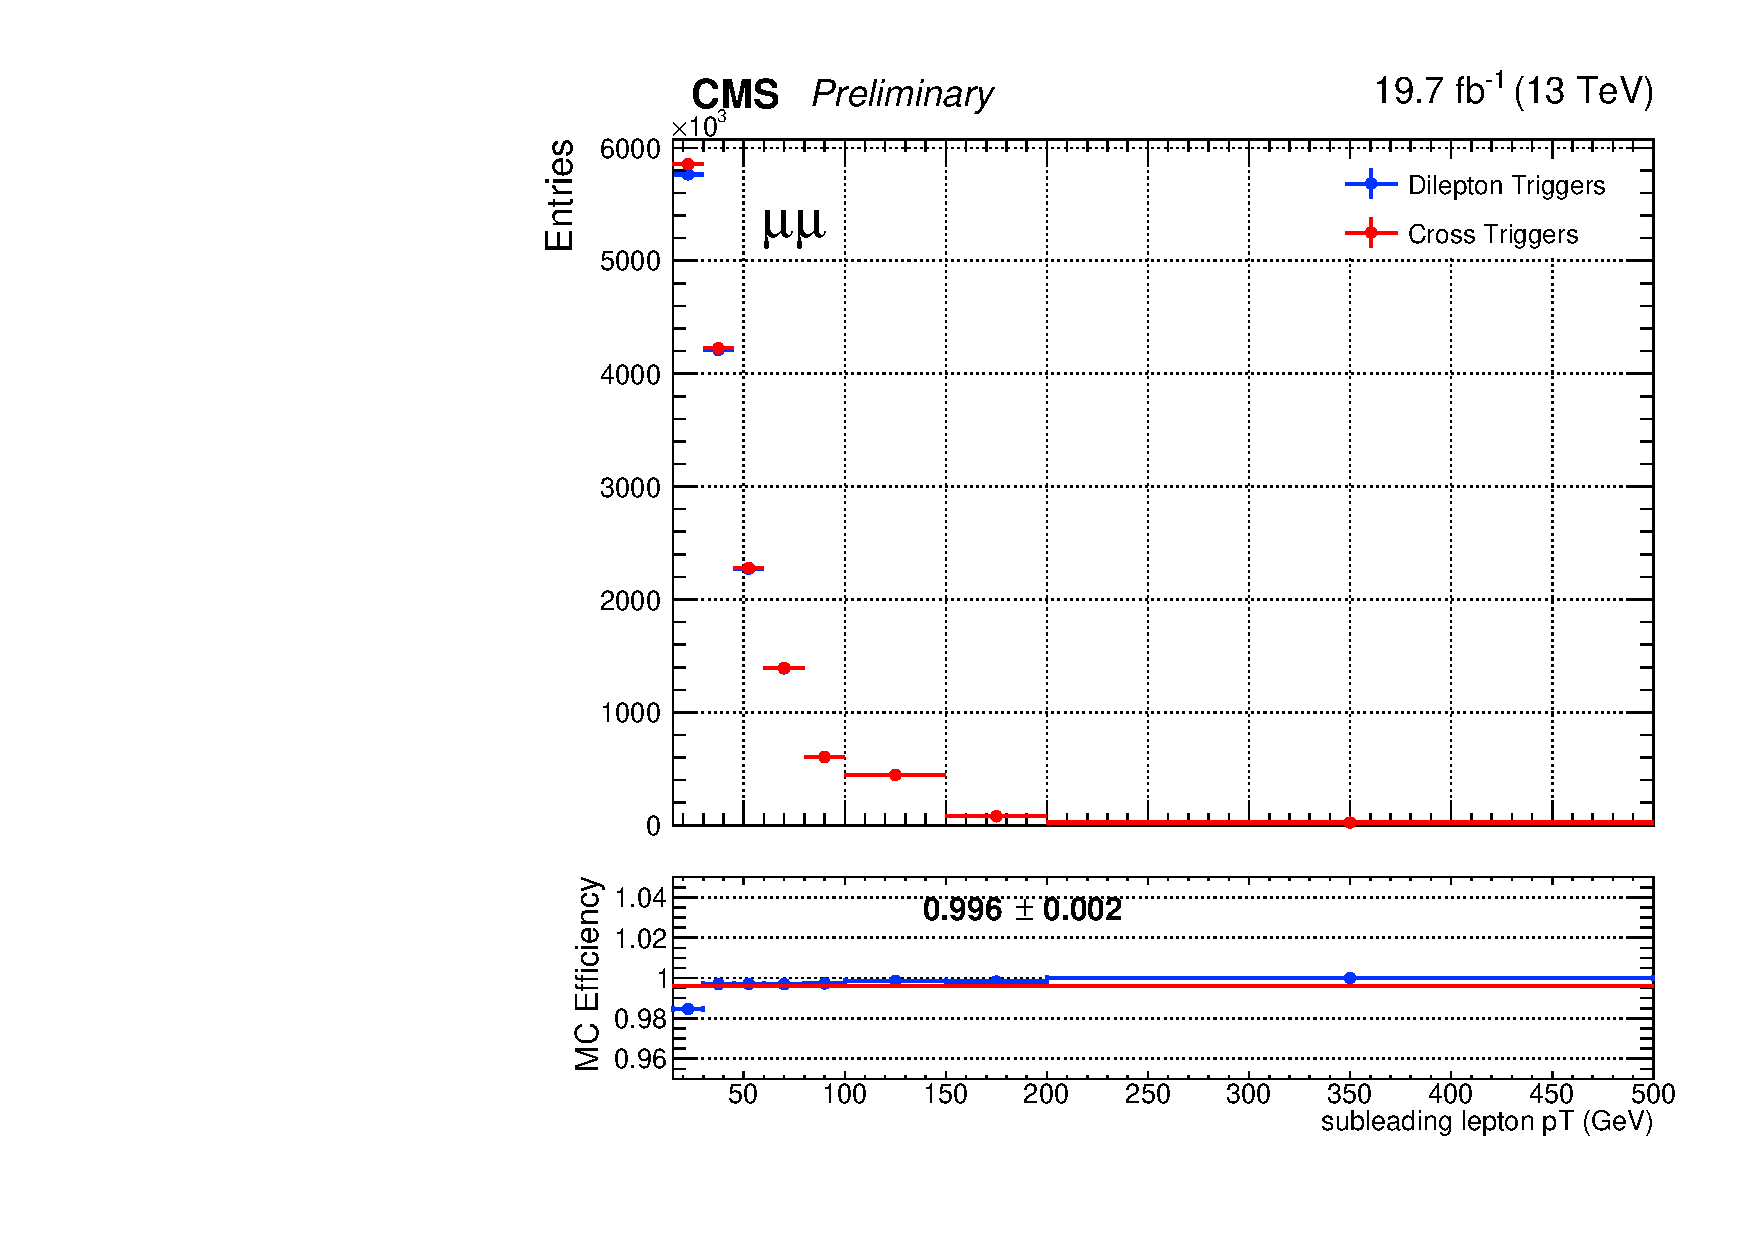
\includegraphics[width=0.32\textwidth]{fig_2016preVFP_TrigSF/g_lepBpt_mumu_MC.pdf}
      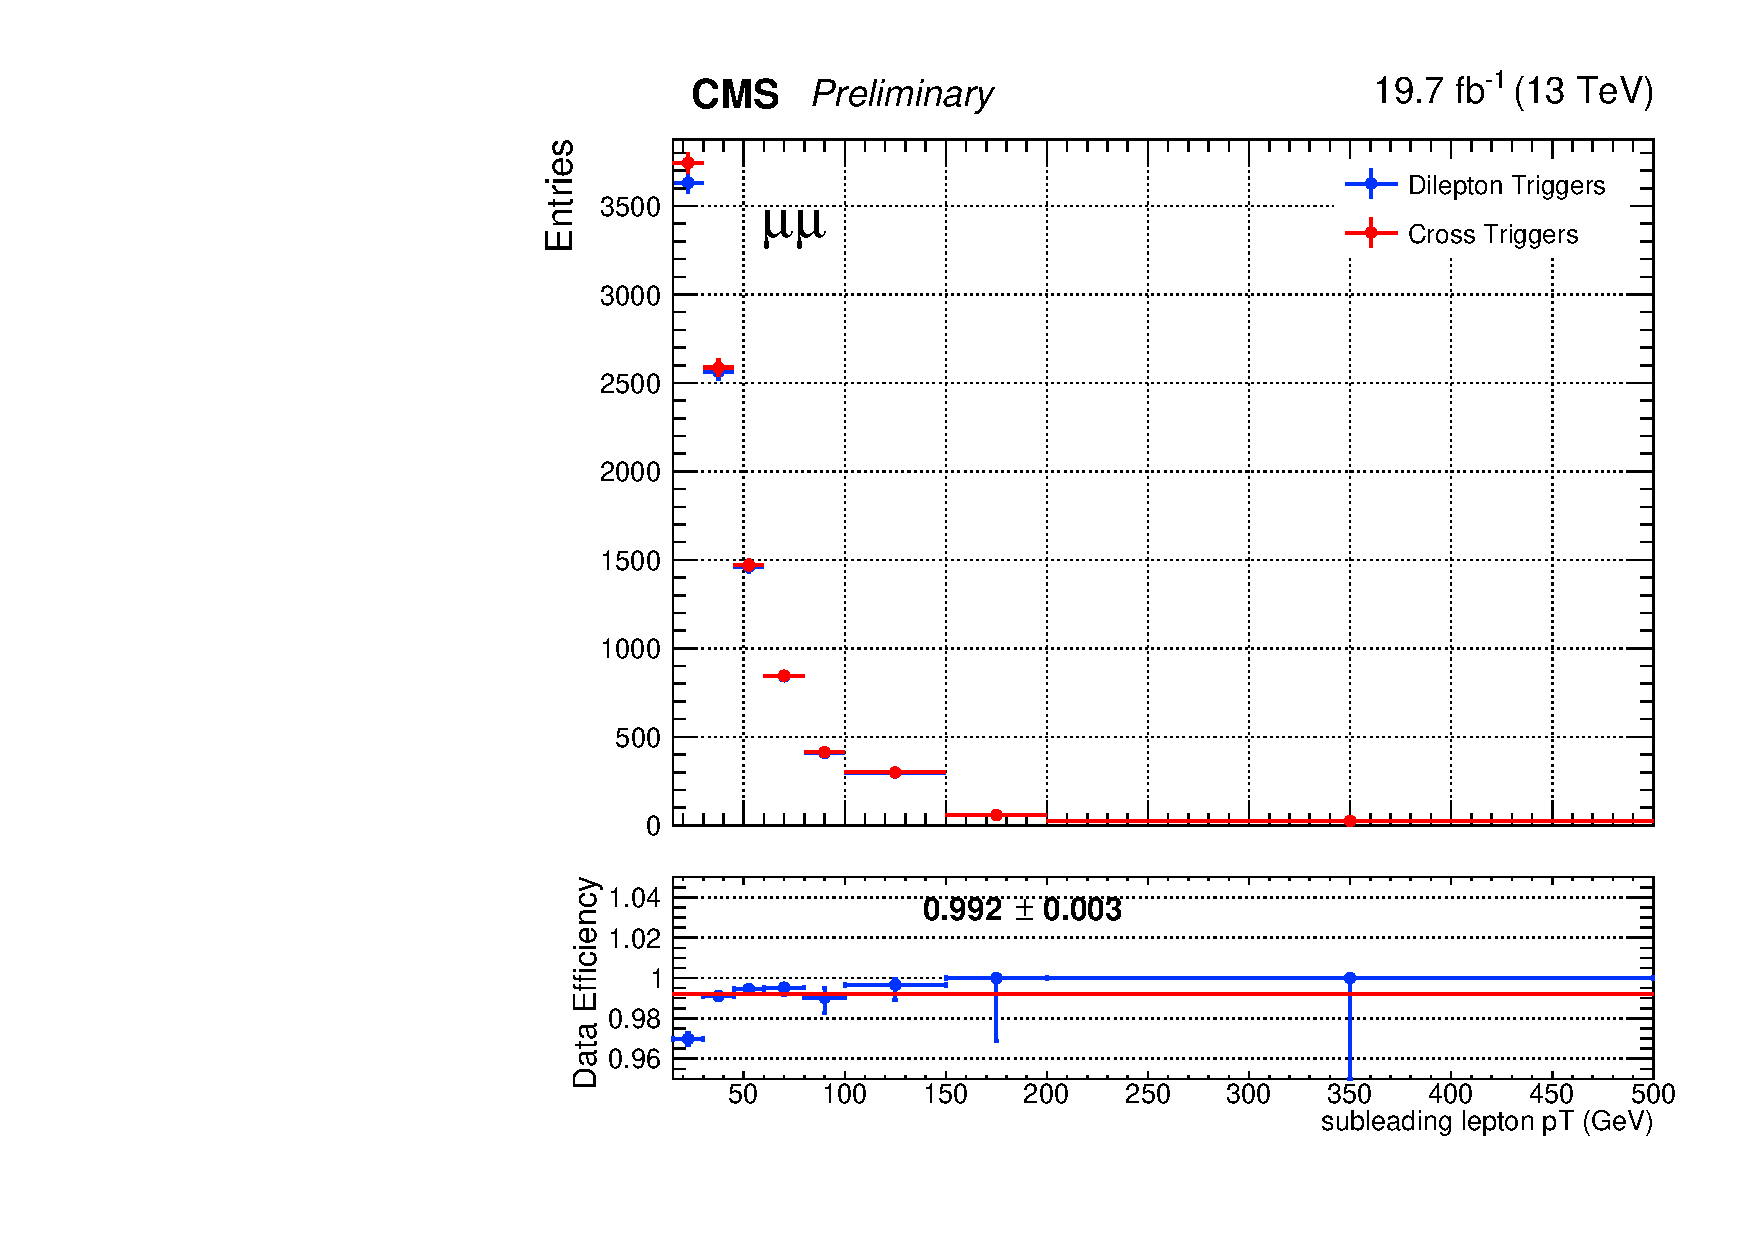
\includegraphics[width=0.32\textwidth]{fig_2016preVFP_TrigSF/g_lepBpt_mumu_data.pdf}
      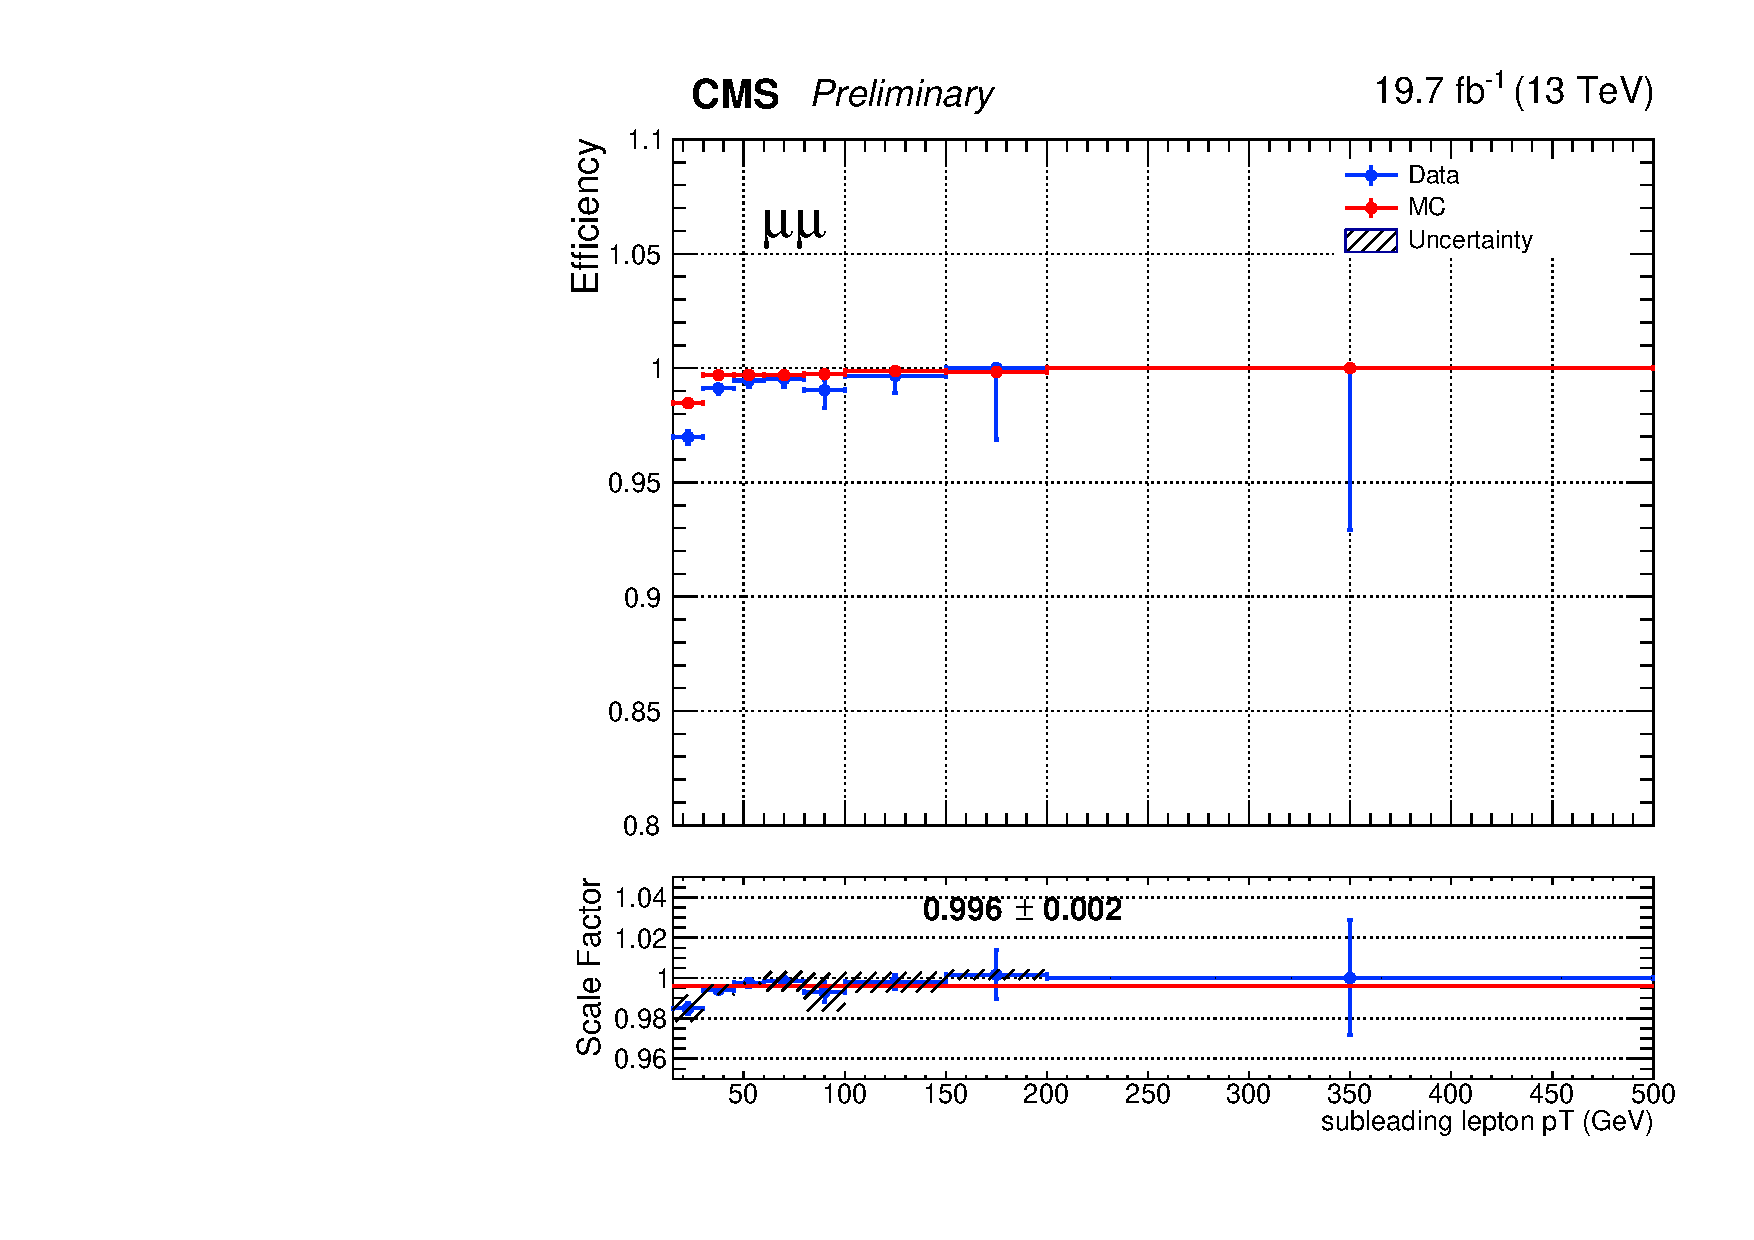
\includegraphics[width=0.32\textwidth]{fig_2016preVFP_TrigSF/g_mumu_lepBpt_FullSystUncBand.pdf}\\
    \end{tabular}
    \caption{Efficiencies and scale factors for the 2016preVFP data set in the $\mu\mu$ channel as a function of leading and sub-leading lepton \pT.
            The error bars indicate the statistical uncertainty, and the shaded band corresponds to the systematic uncertainty.
            }
    \label{TrigSF_2016preVFP_3}
  \end{center}
\end{figure}

\begin{figure}[h]
  \begin{center}
    \begin{tabular}{cc}
      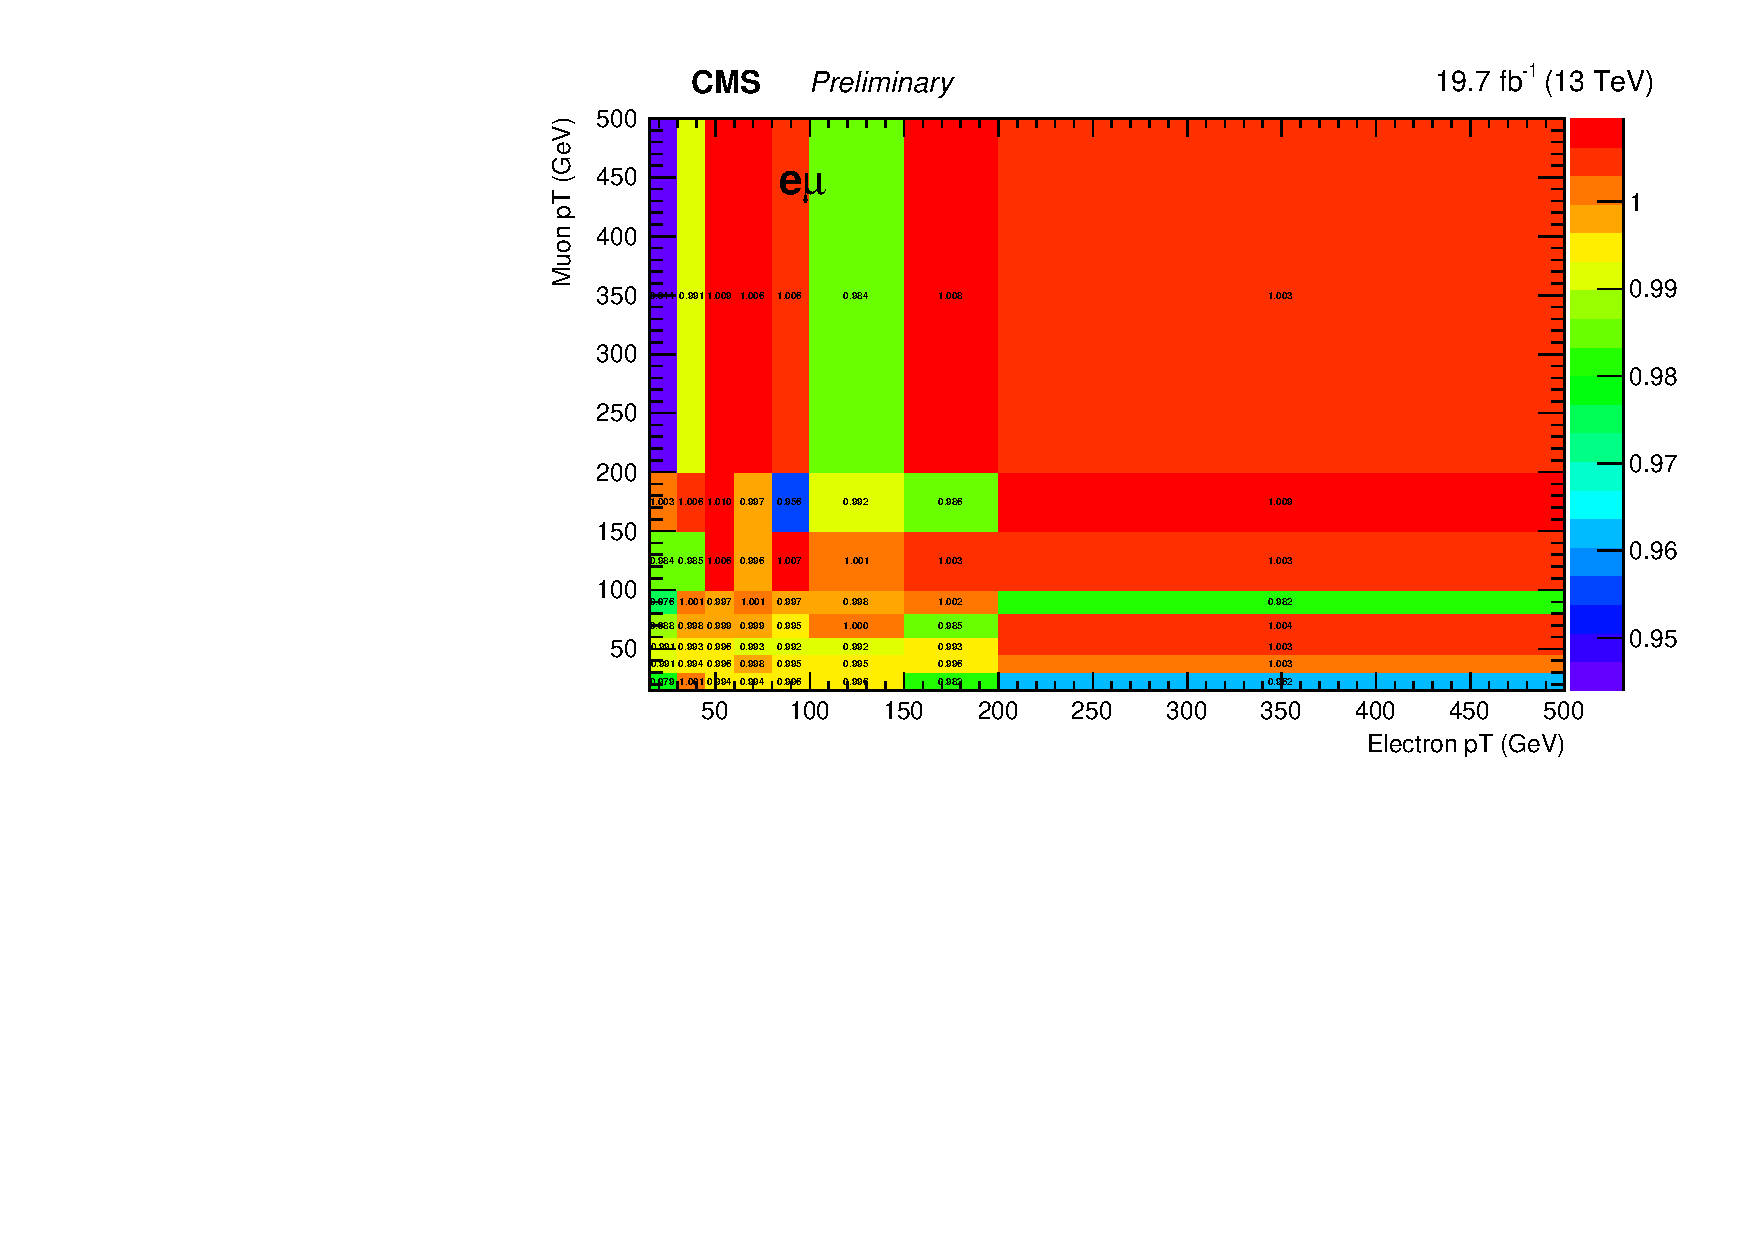
\includegraphics[width=0.50\textwidth]{fig_2016preVFP_TrigSF/h2D_lepABpt_emu.pdf}
      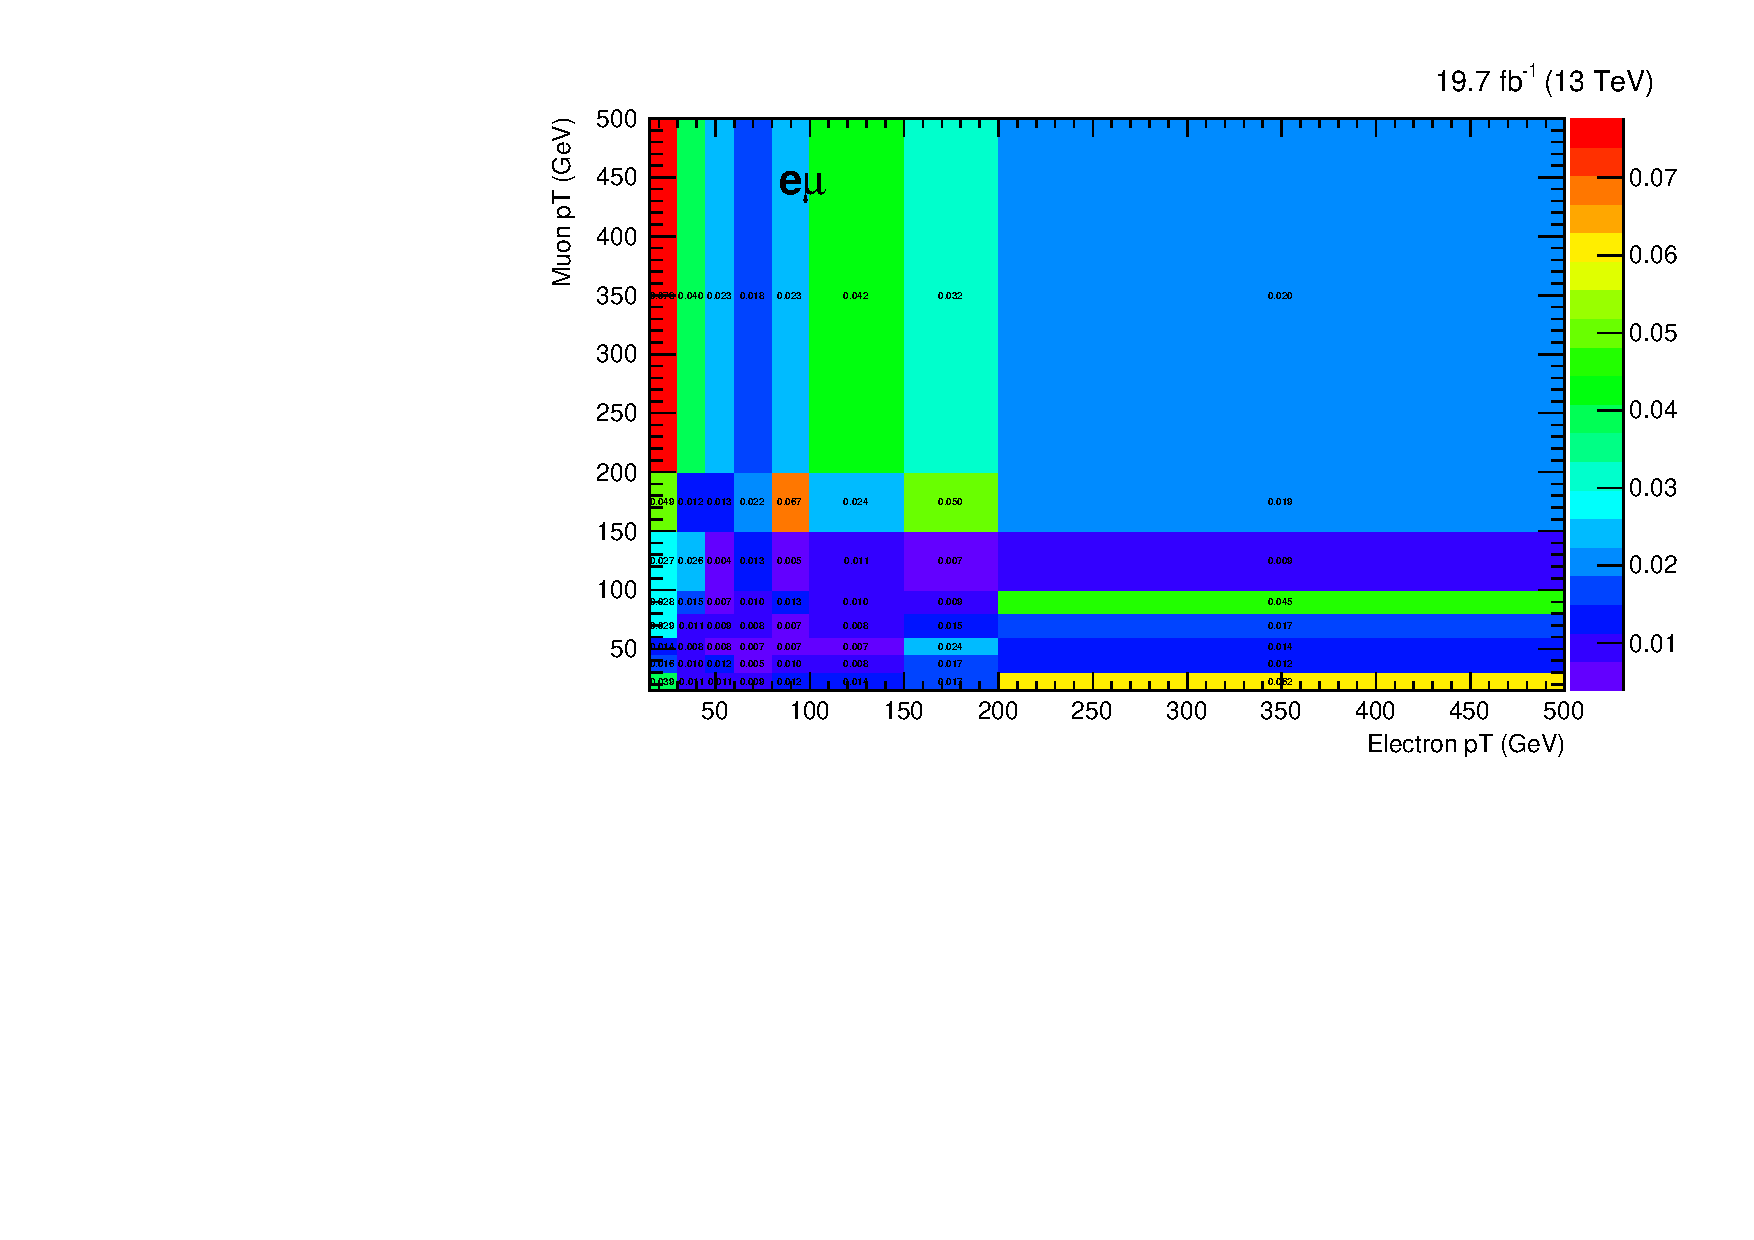
\includegraphics[width=0.50\textwidth]{fig_2016preVFP_TrigSF/h2D_lepABpt_emu_BinErrors.pdf}\\       
      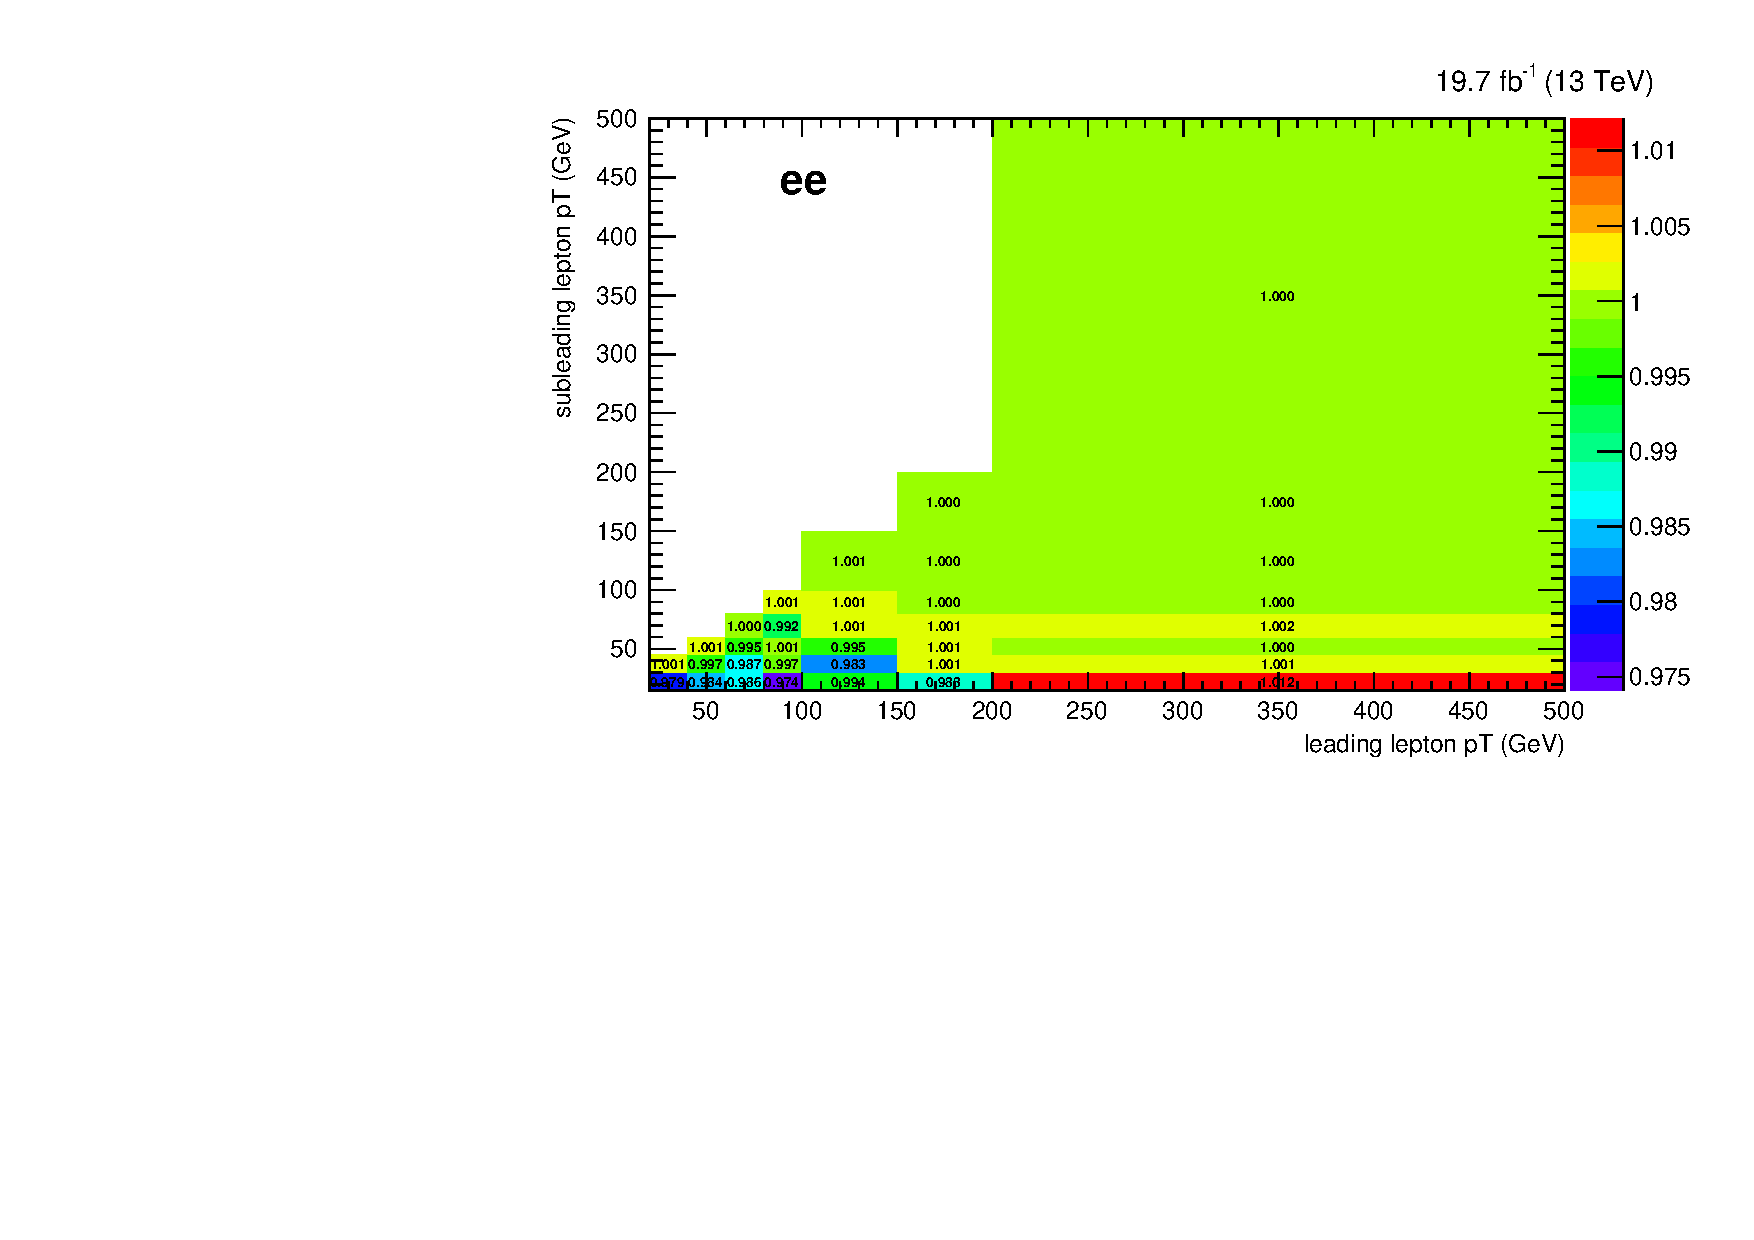
\includegraphics[width=0.50\textwidth]{fig_2016preVFP_TrigSF/h2D_lepABpt_ee.pdf}
      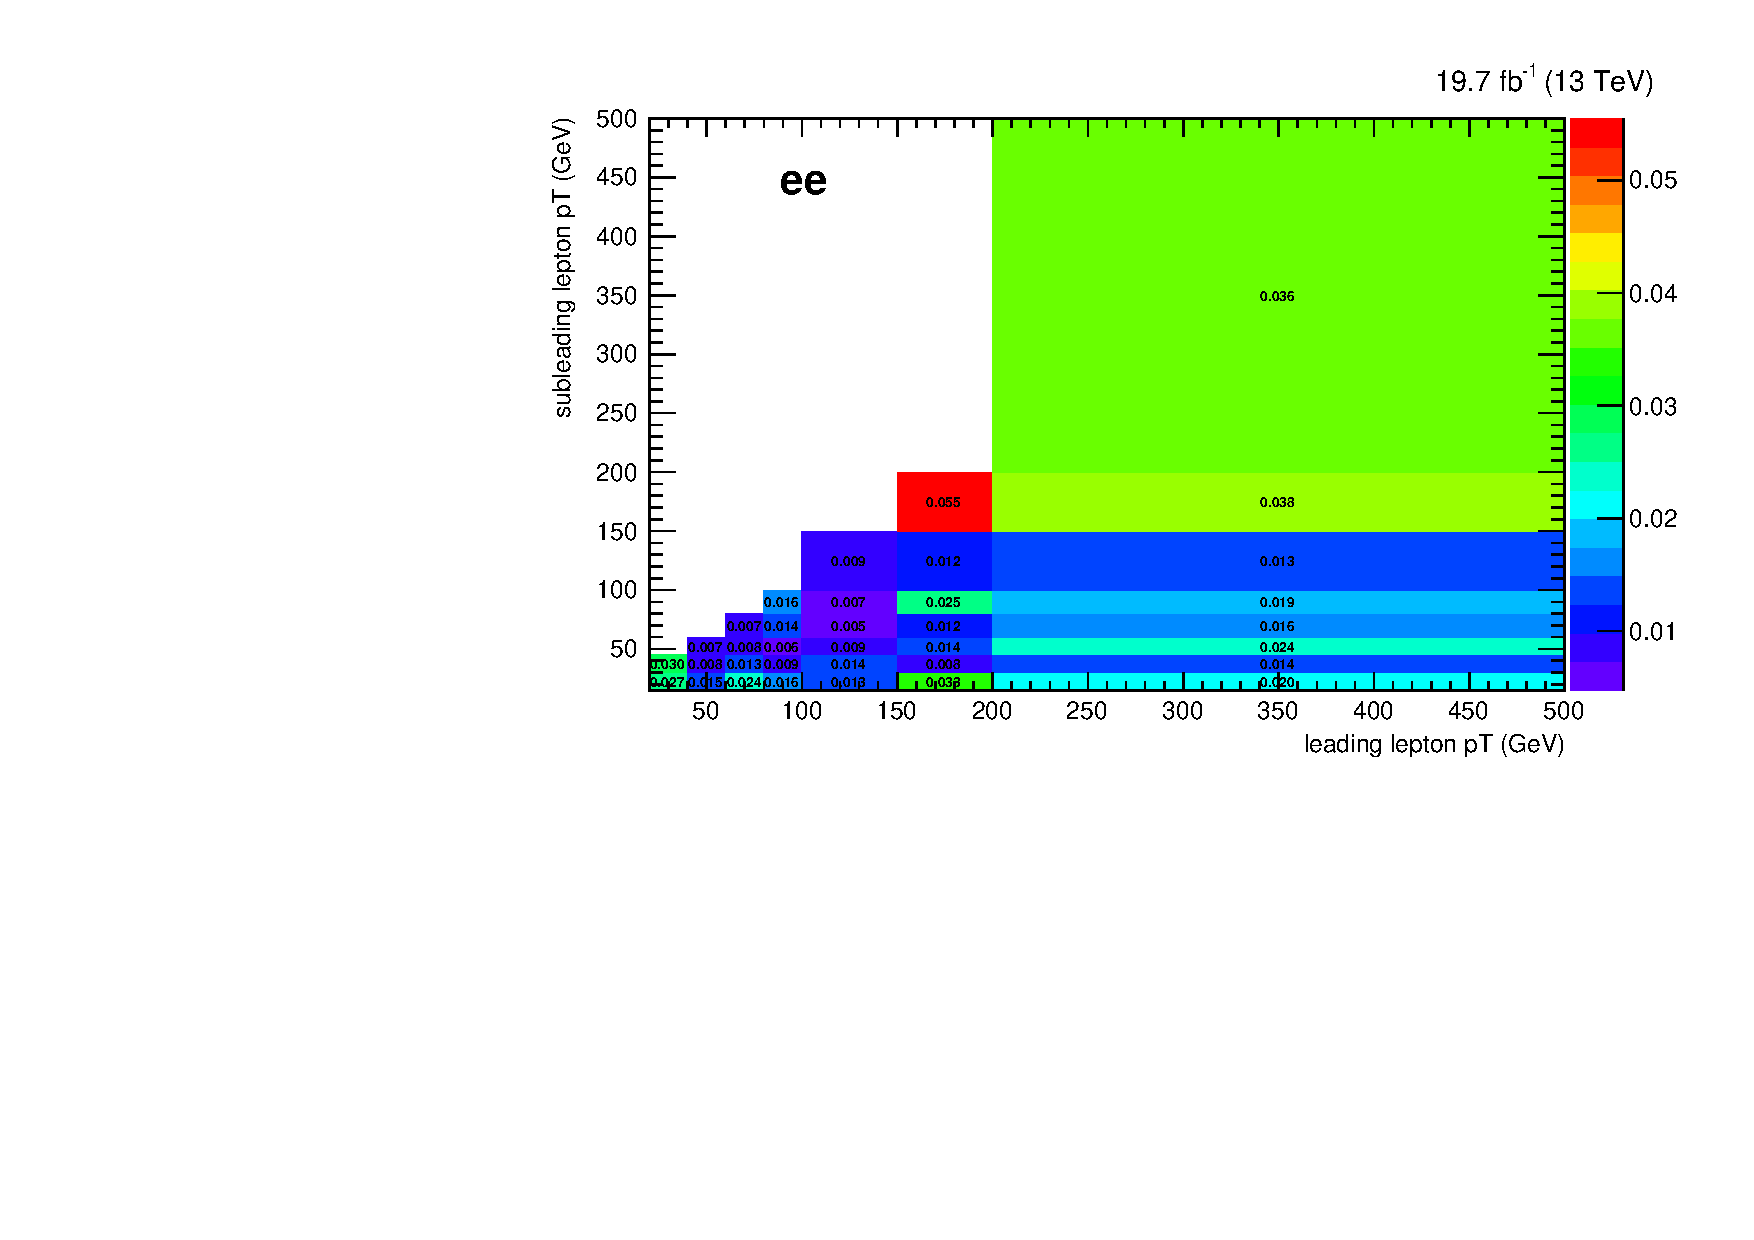
\includegraphics[width=0.50\textwidth]{fig_2016preVFP_TrigSF/h2D_lepABpt_ee_BinErrors.pdf}\\
      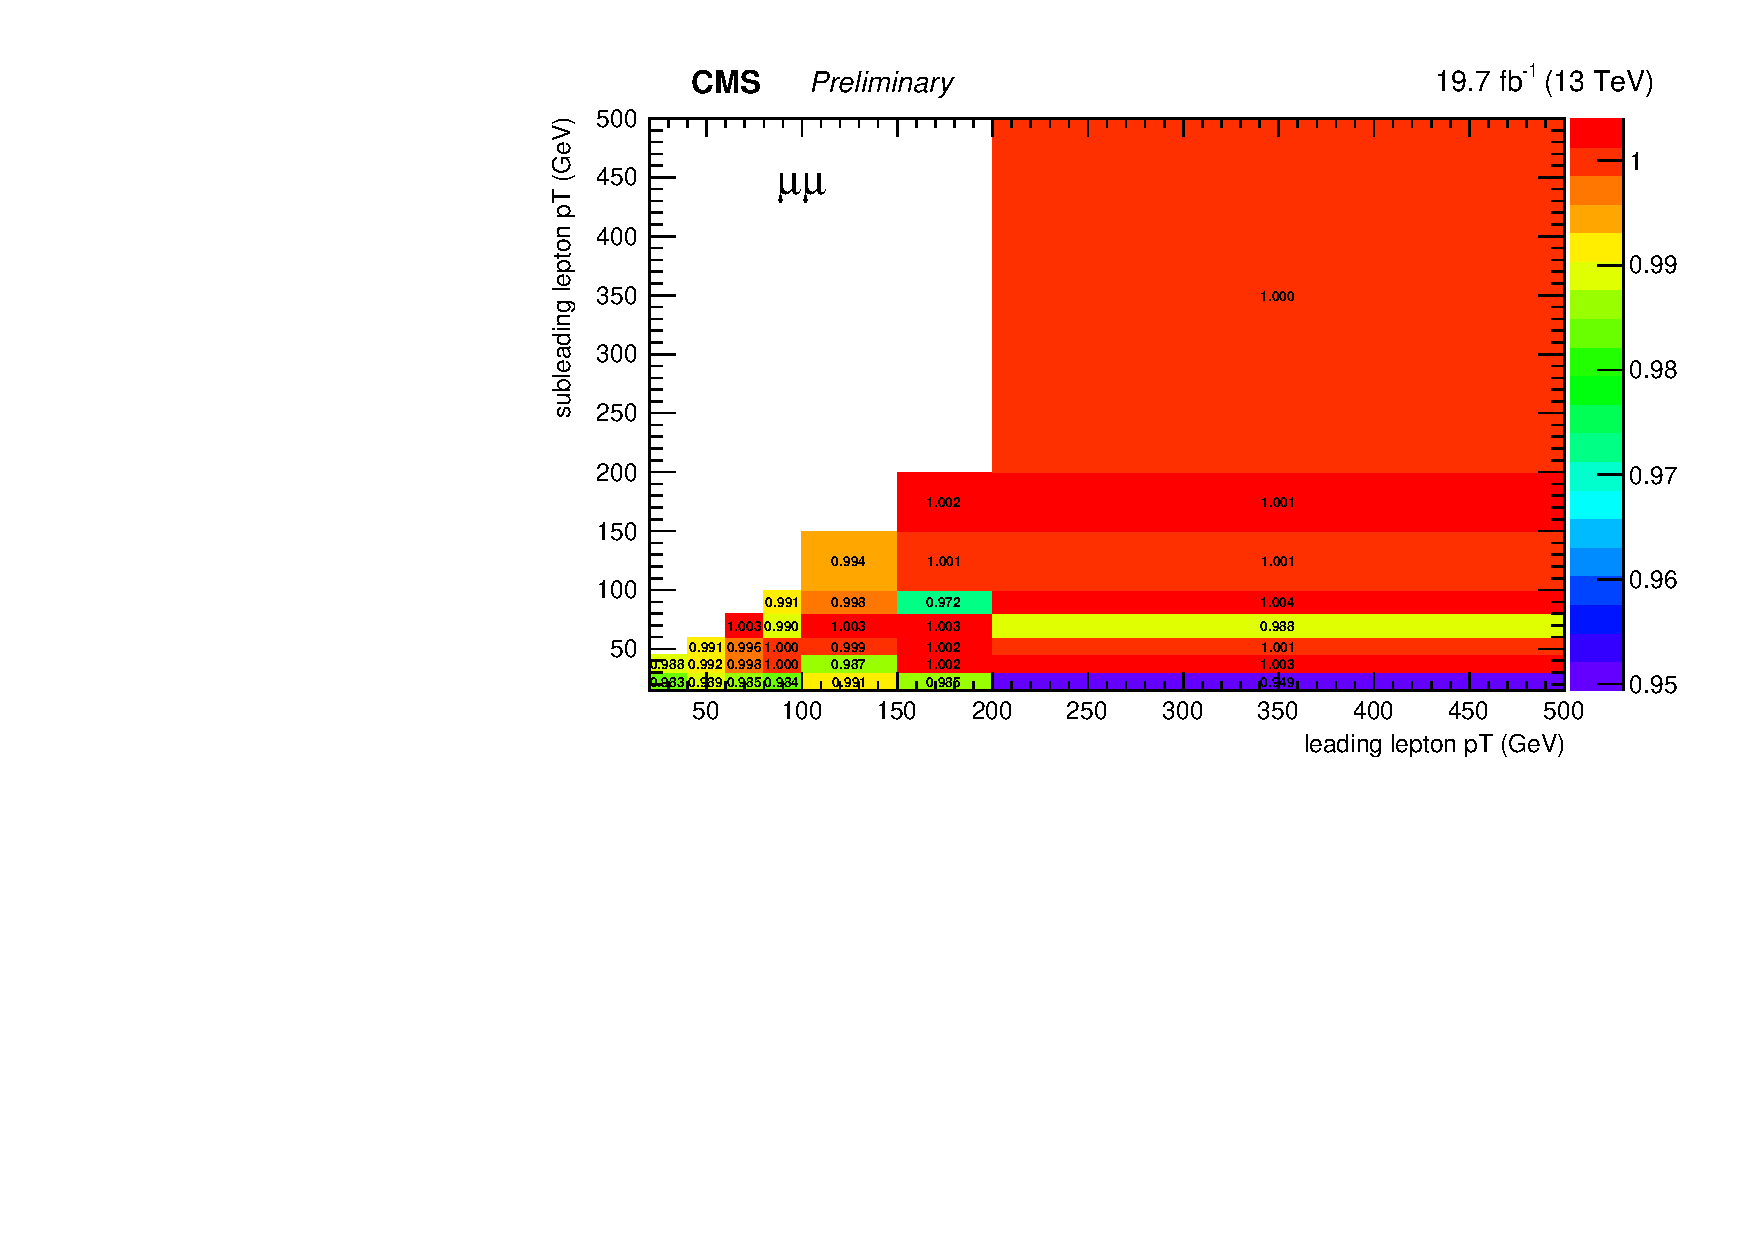
\includegraphics[width=0.50\textwidth]{fig_2016preVFP_TrigSF/h2D_lepABpt_mumu.pdf}
      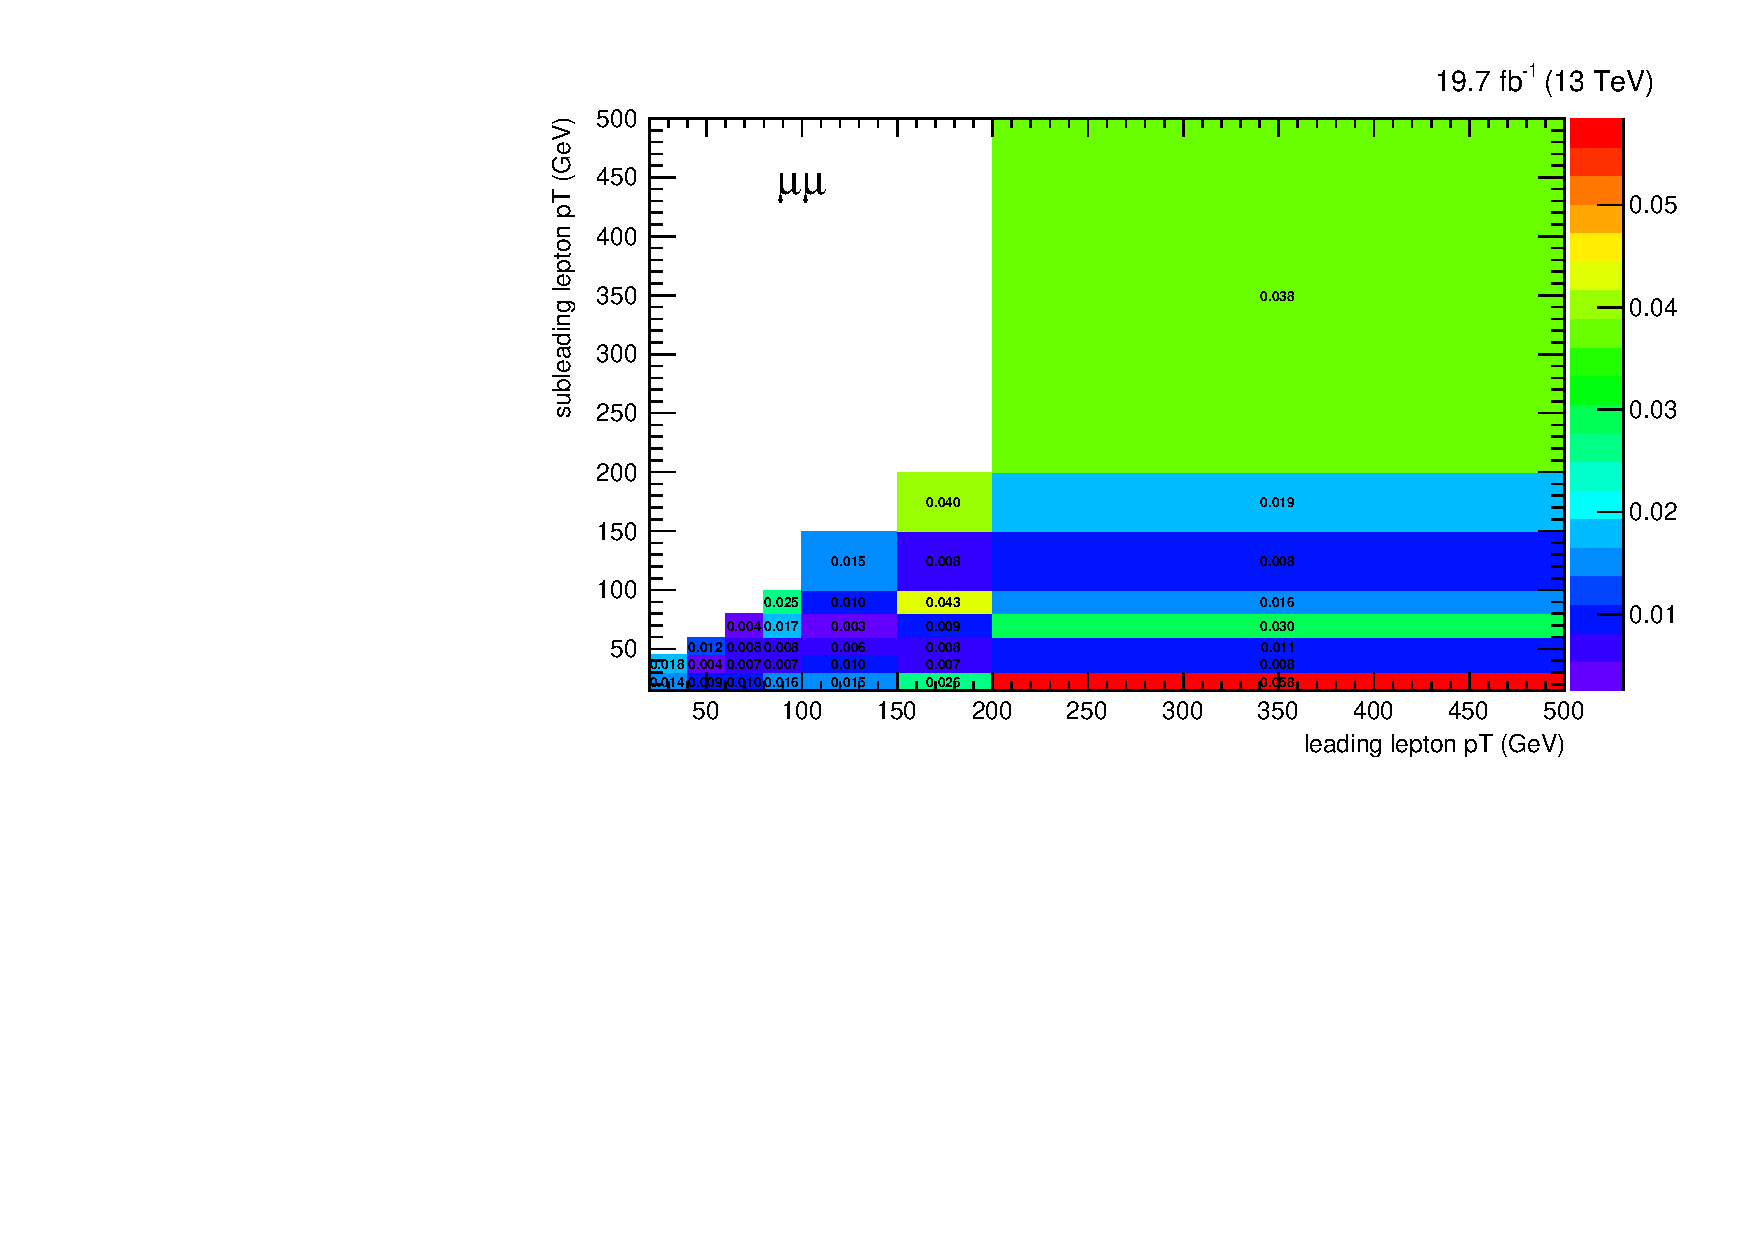
\includegraphics[width=0.50\textwidth]{fig_2016preVFP_TrigSF/h2D_lepABpt_mumu_BinErrors.pdf}\\
    \end{tabular}
    \caption{2D scale factors (Left) and total uncertainties (Right) for the 2016preVFP data set in the $e\mu$ (top), $ee$ (middle) and $\mu\mu$ (bottom) channels as a function of leading lepton \pT and sub-leading lepton \pT.}
    \label{TrigSF_2016preVFP_4}
  \end{center}
\end{figure}

\clearpage
\subsection{Trigger Efficiencies and Scale Factors: 2016postVFP}
\label{TrigSFResults2016postVFP}

\begin{figure}[h]
  \begin{center}
    \begin{tabular}{ccc}
      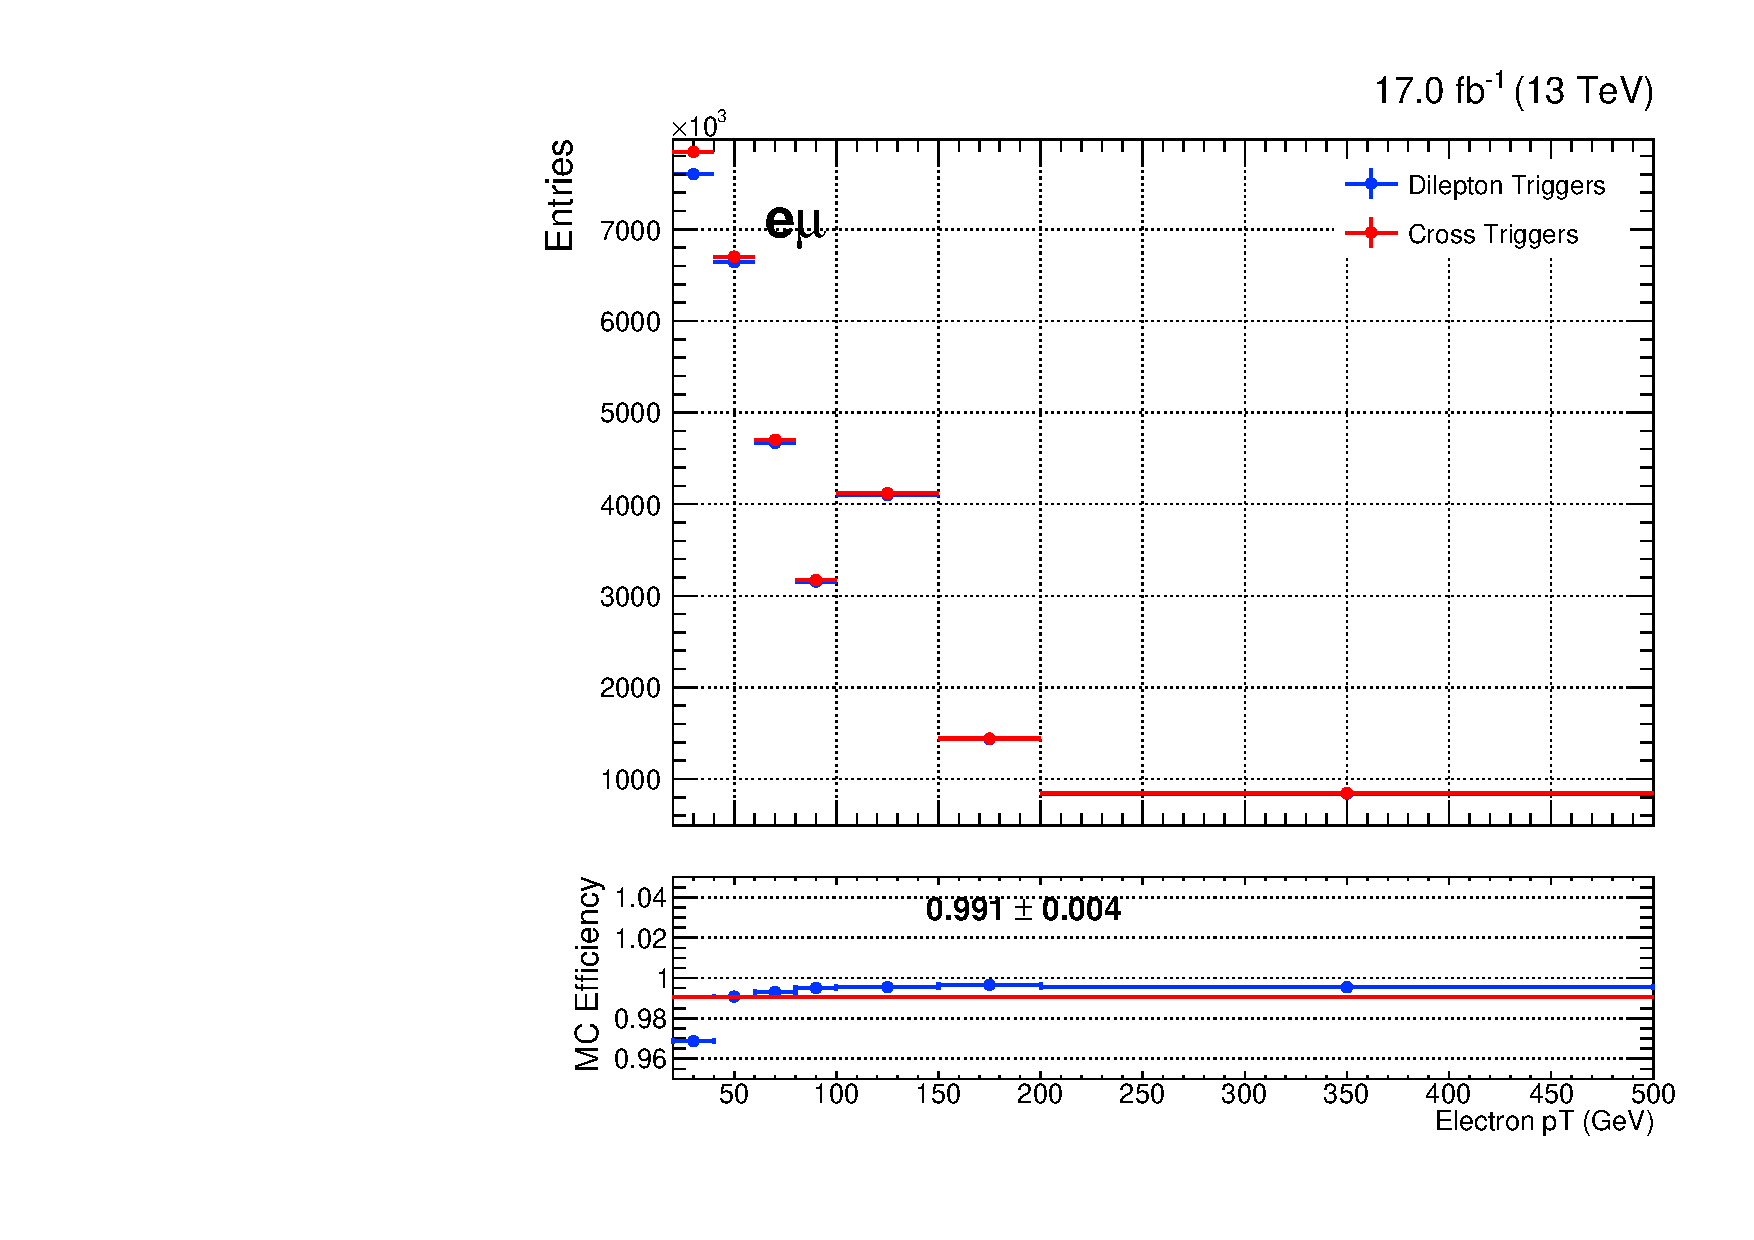
\includegraphics[width=0.32\textwidth]{fig_2016postVFP_TrigSF/g_lepApt_emu_MC.pdf}
      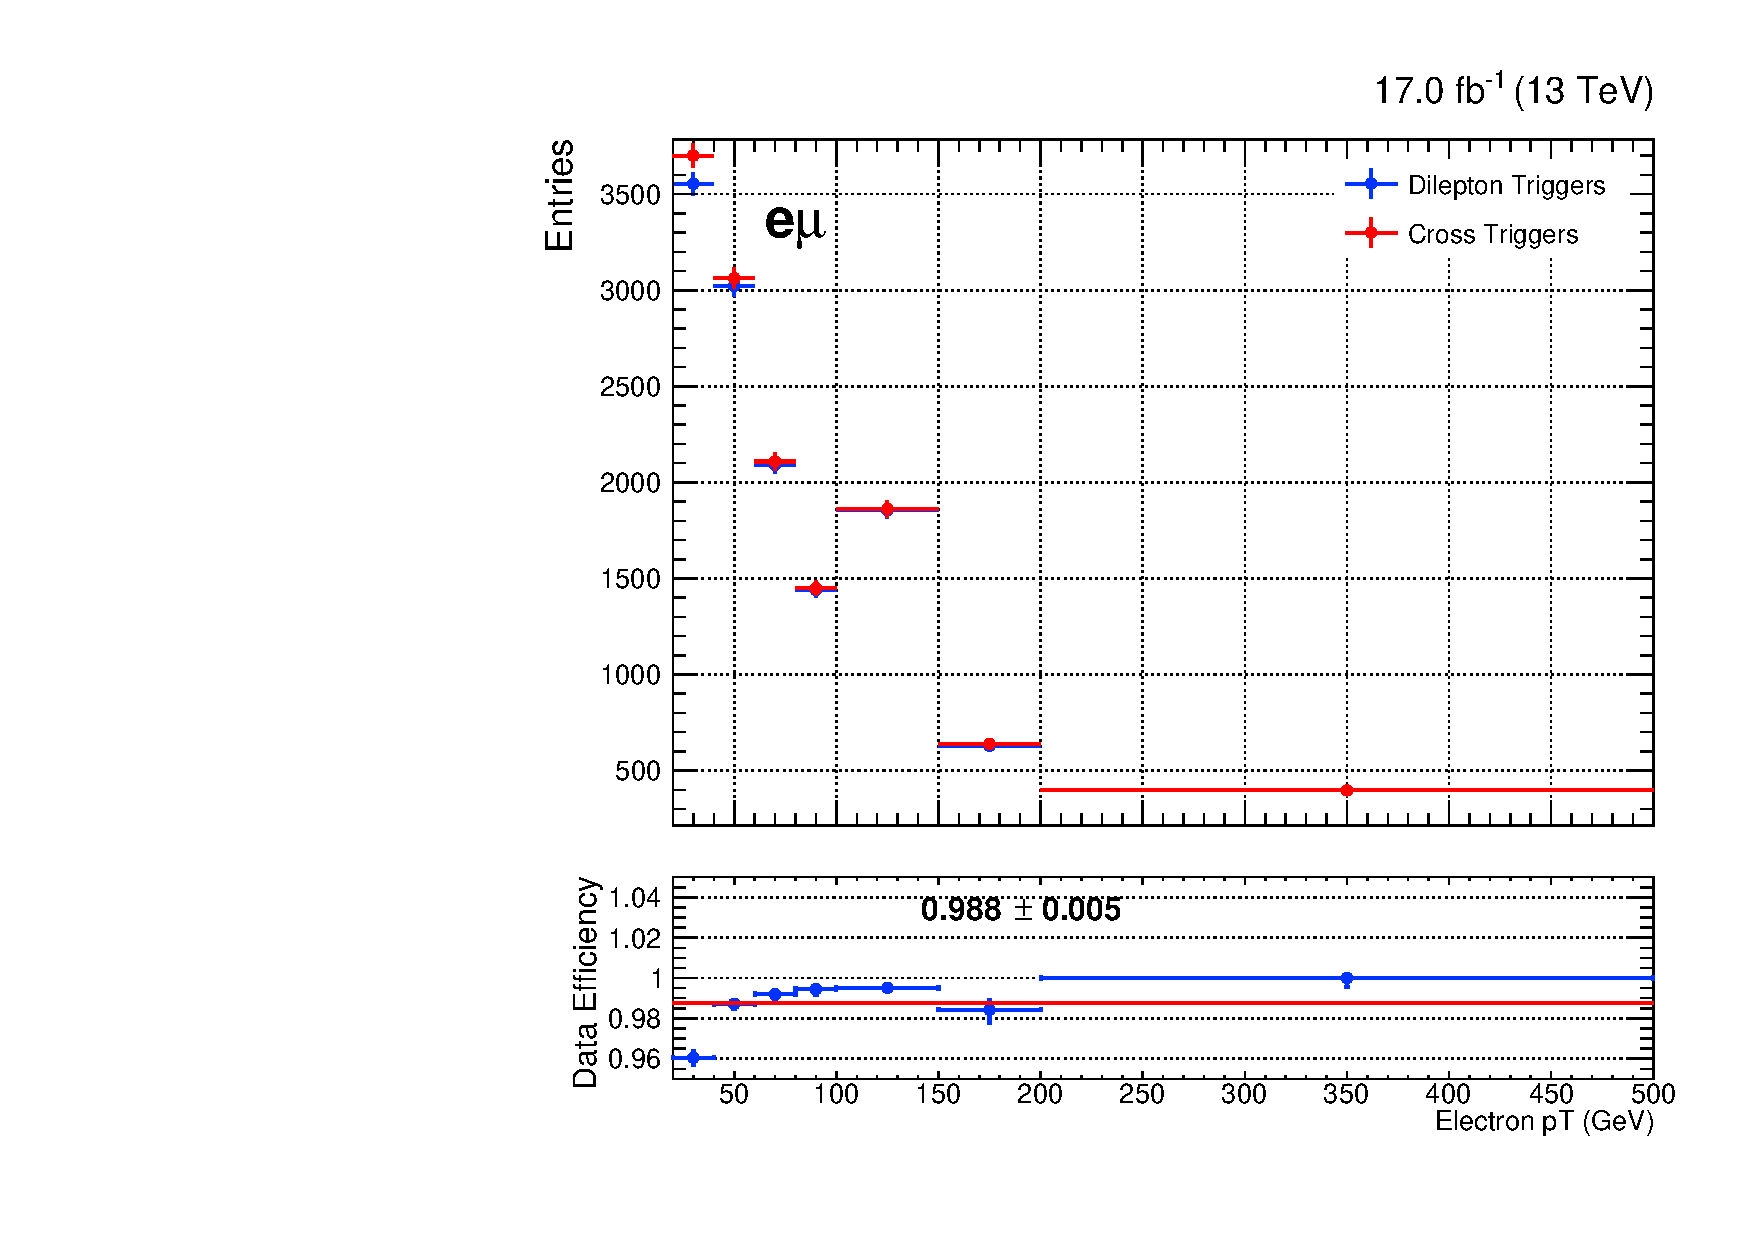
\includegraphics[width=0.32\textwidth]{fig_2016postVFP_TrigSF/g_lepApt_emu_data.pdf}
      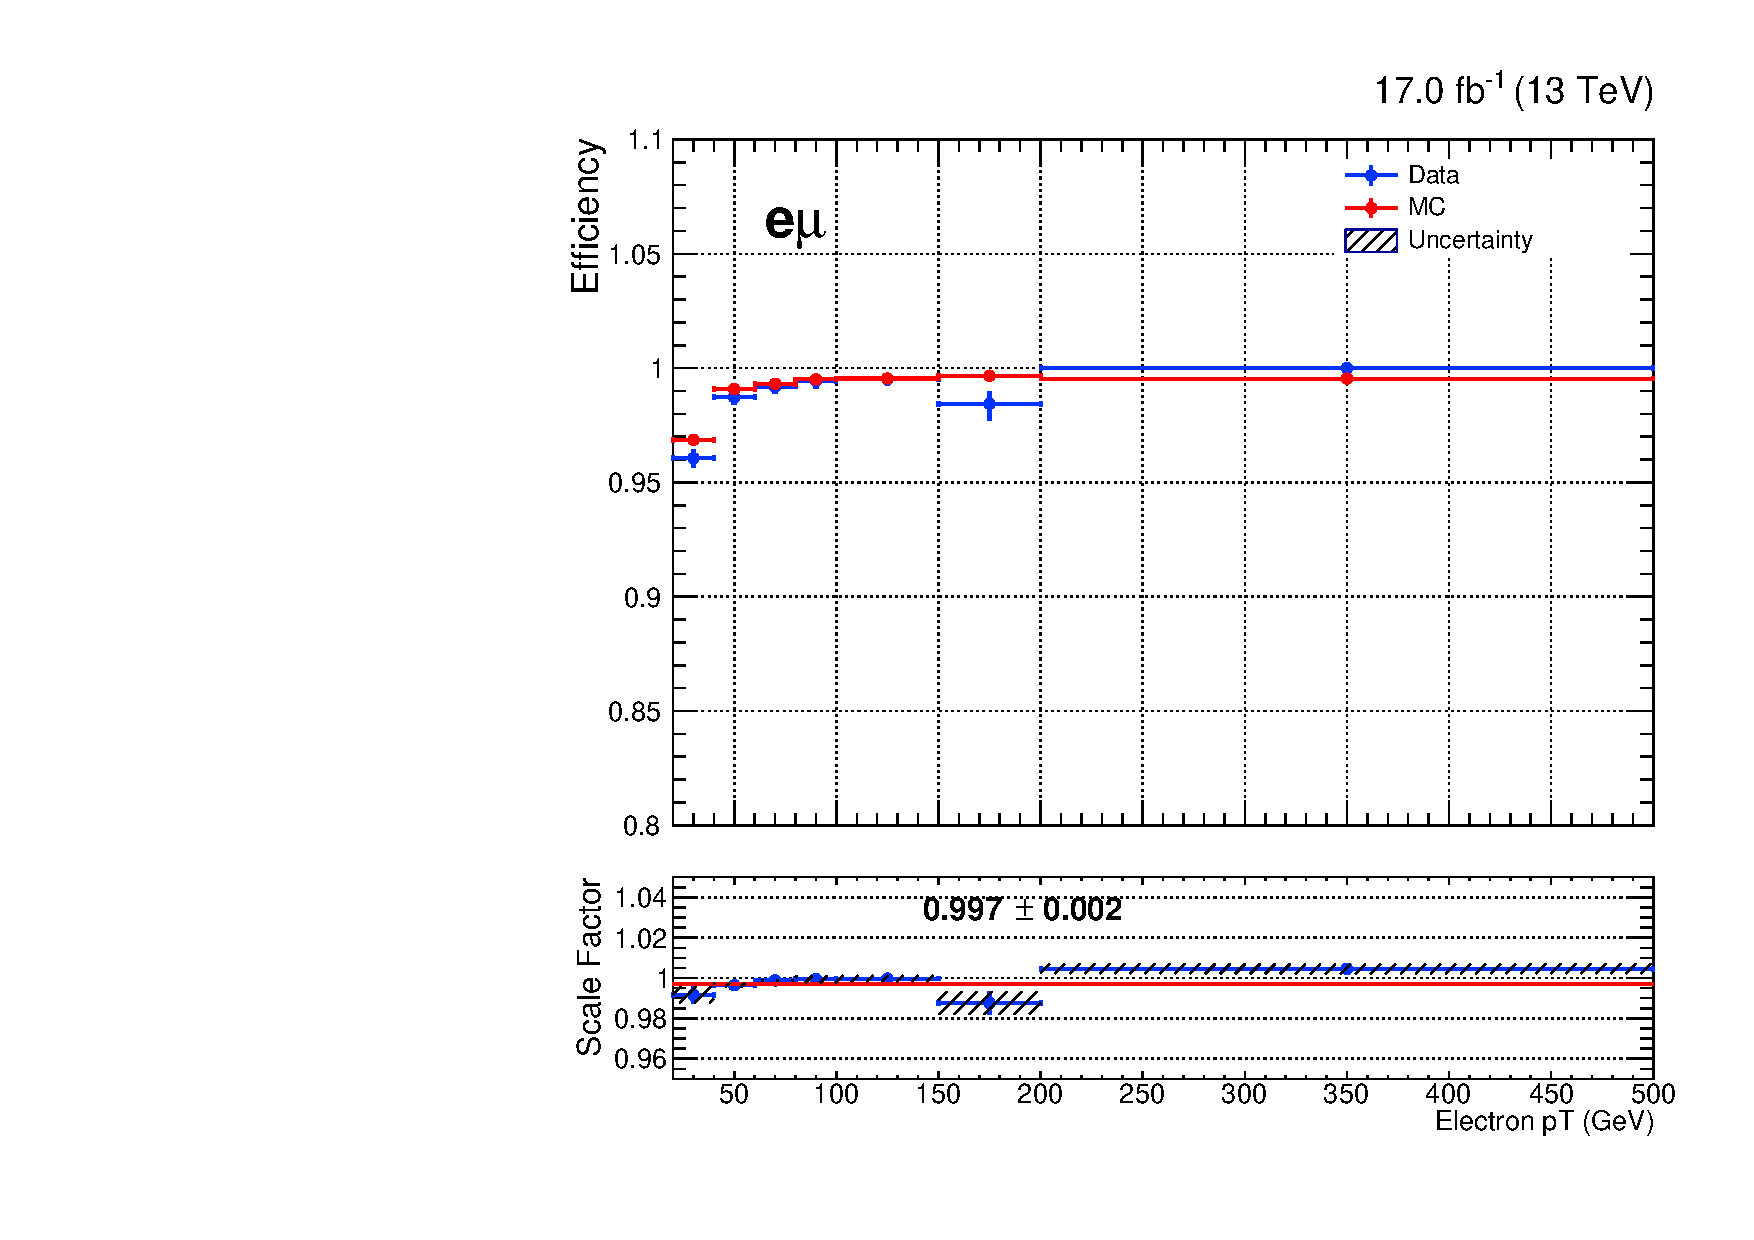
\includegraphics[width=0.32\textwidth]{fig_2016postVFP_TrigSF/g_emu_lepApt_FullSystUncBand.pdf}\\
      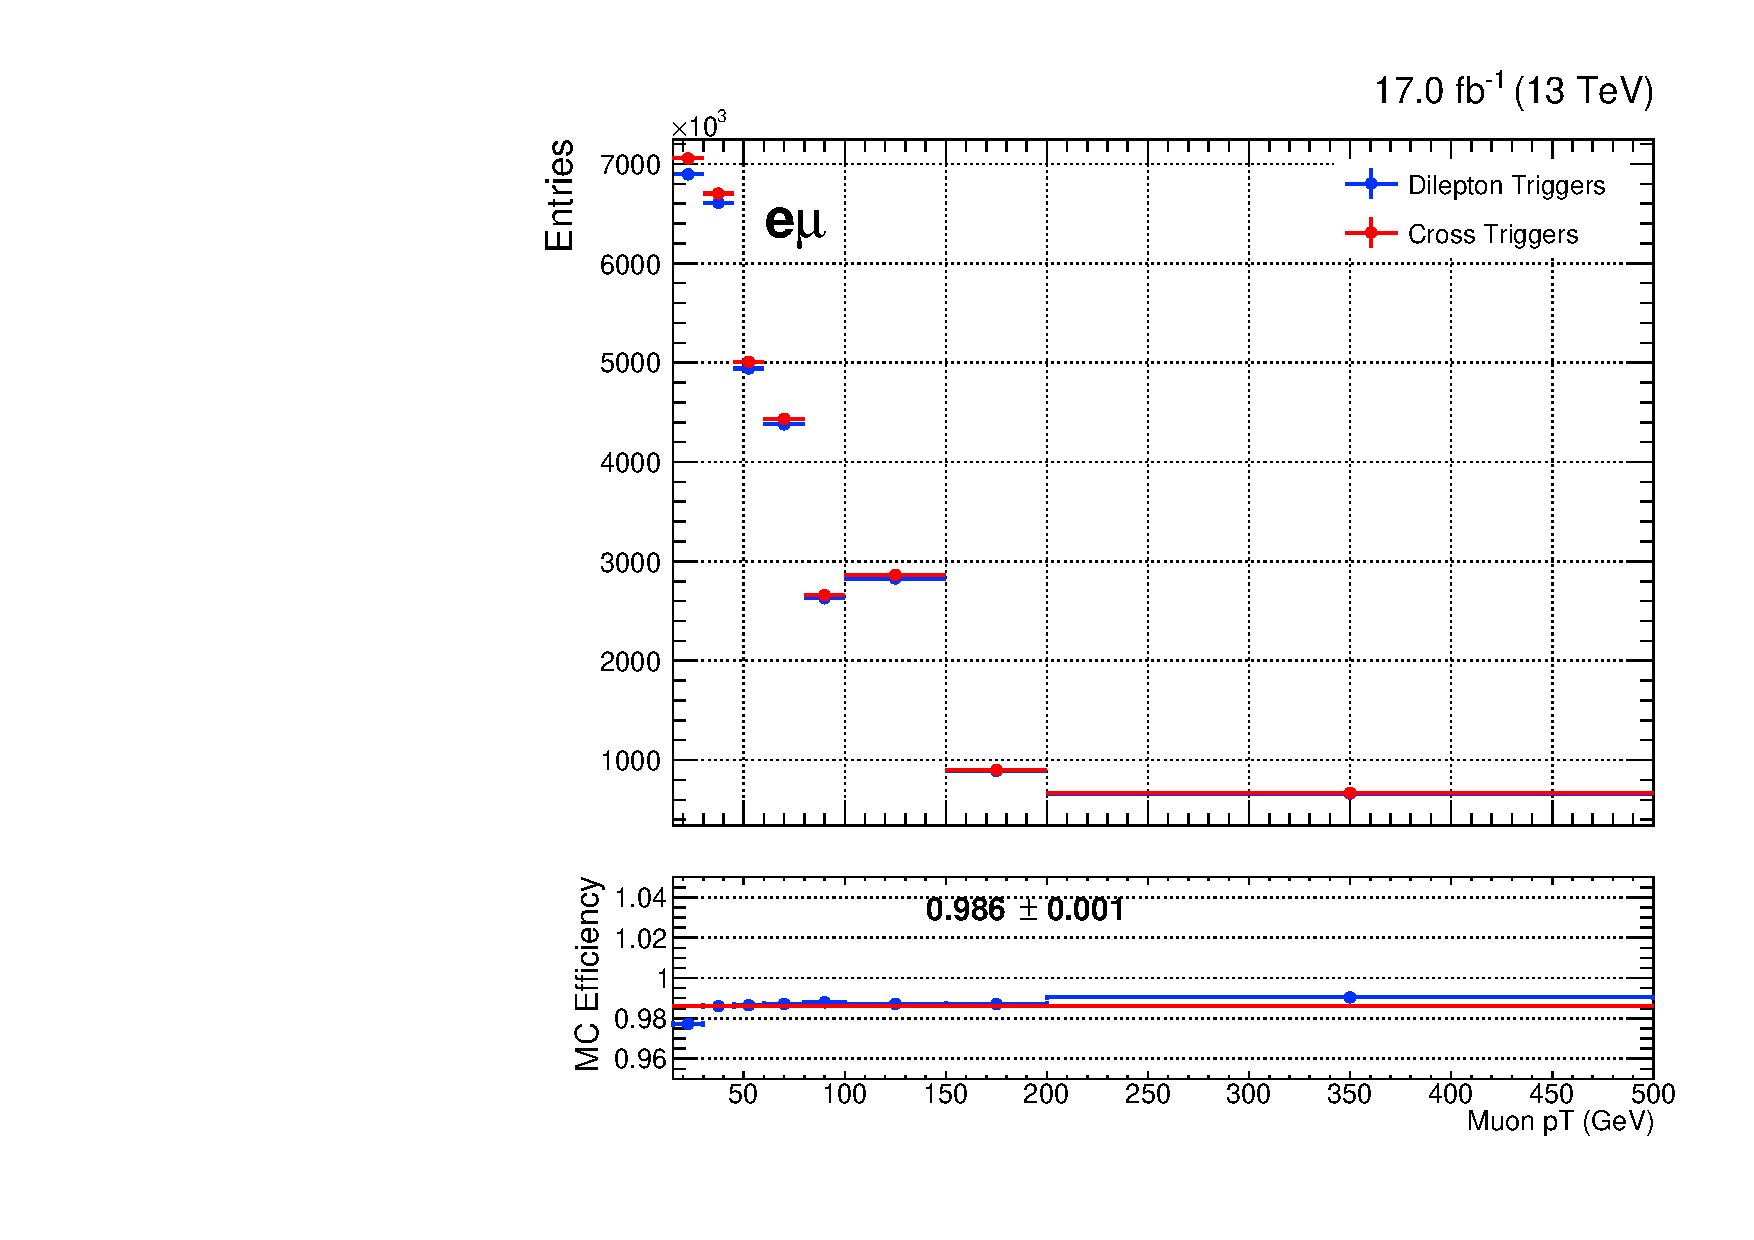
\includegraphics[width=0.32\textwidth]{fig_2016postVFP_TrigSF/g_lepBpt_emu_MC.pdf}
      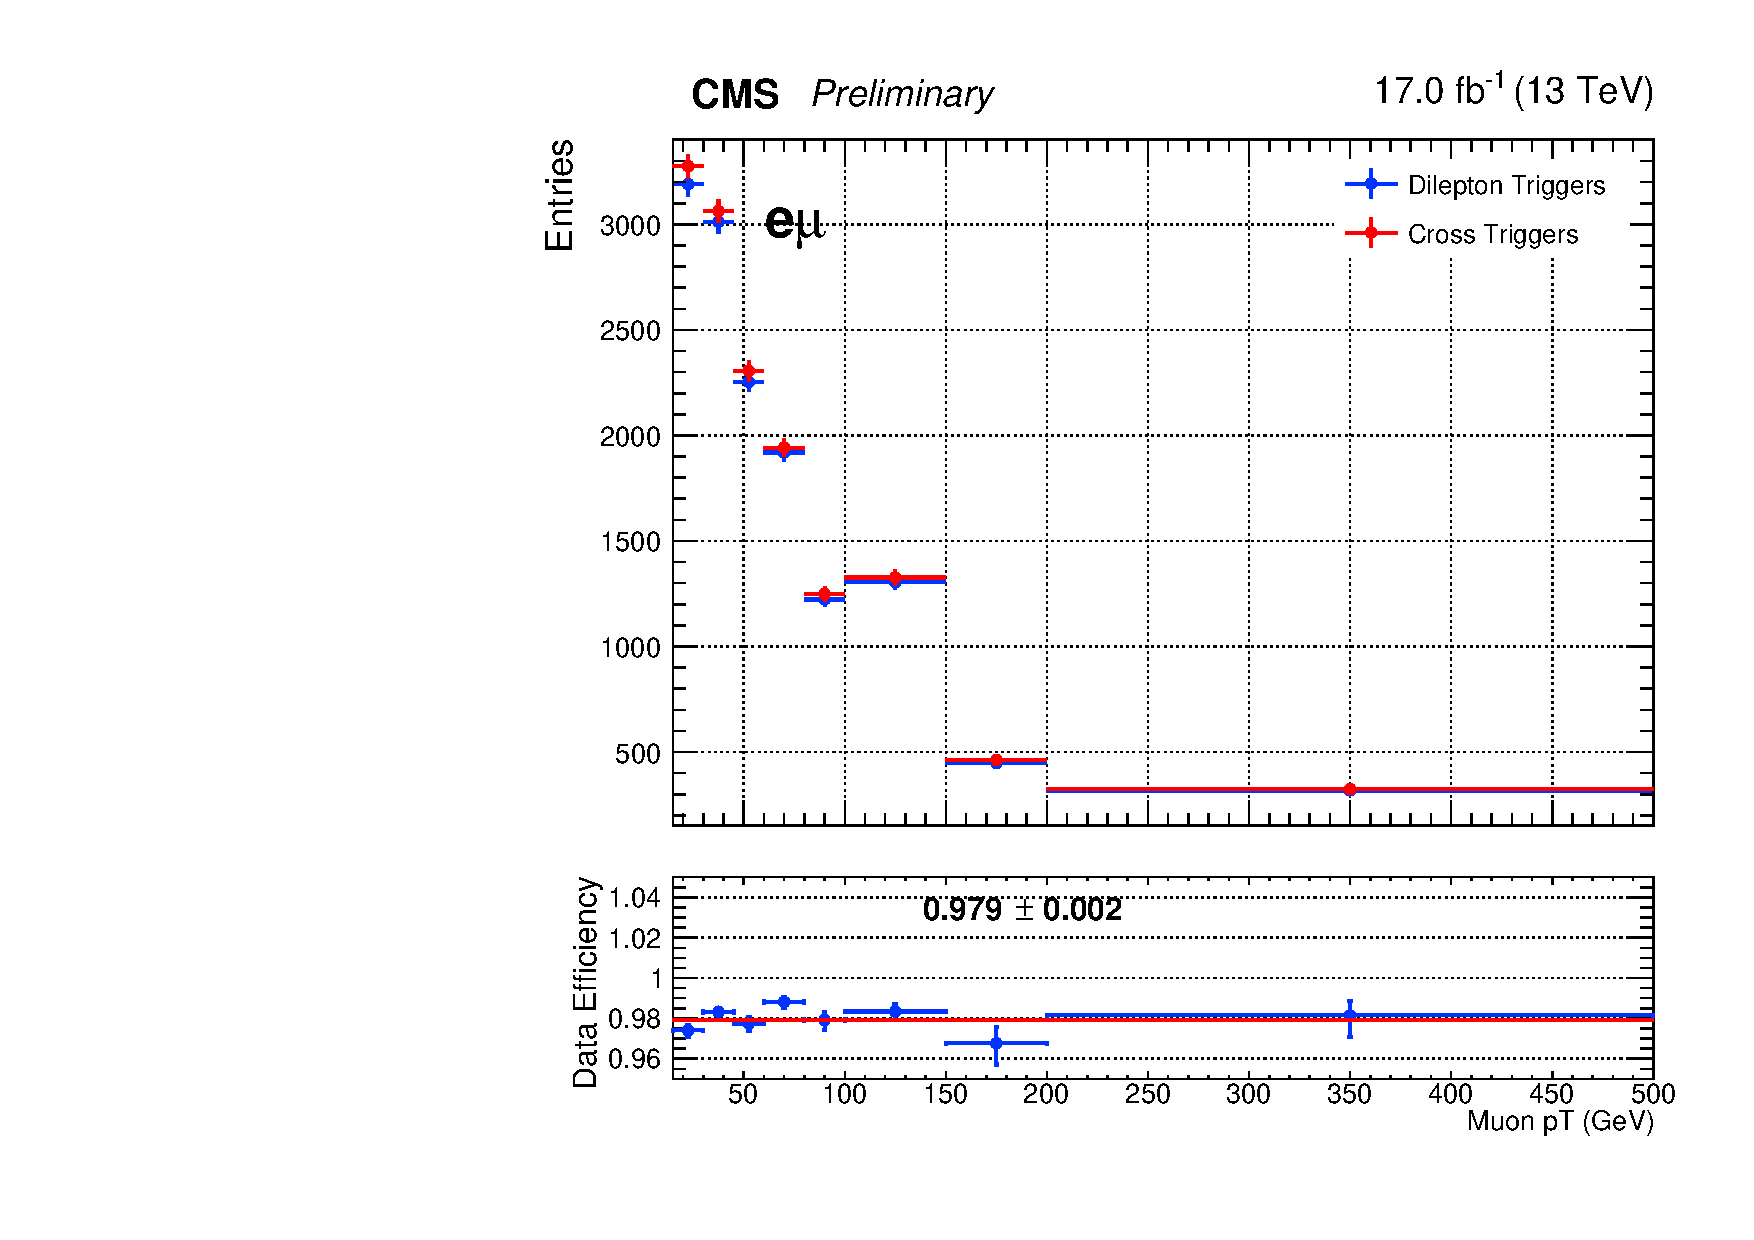
\includegraphics[width=0.32\textwidth]{fig_2016postVFP_TrigSF/g_lepBpt_emu_data.pdf}
      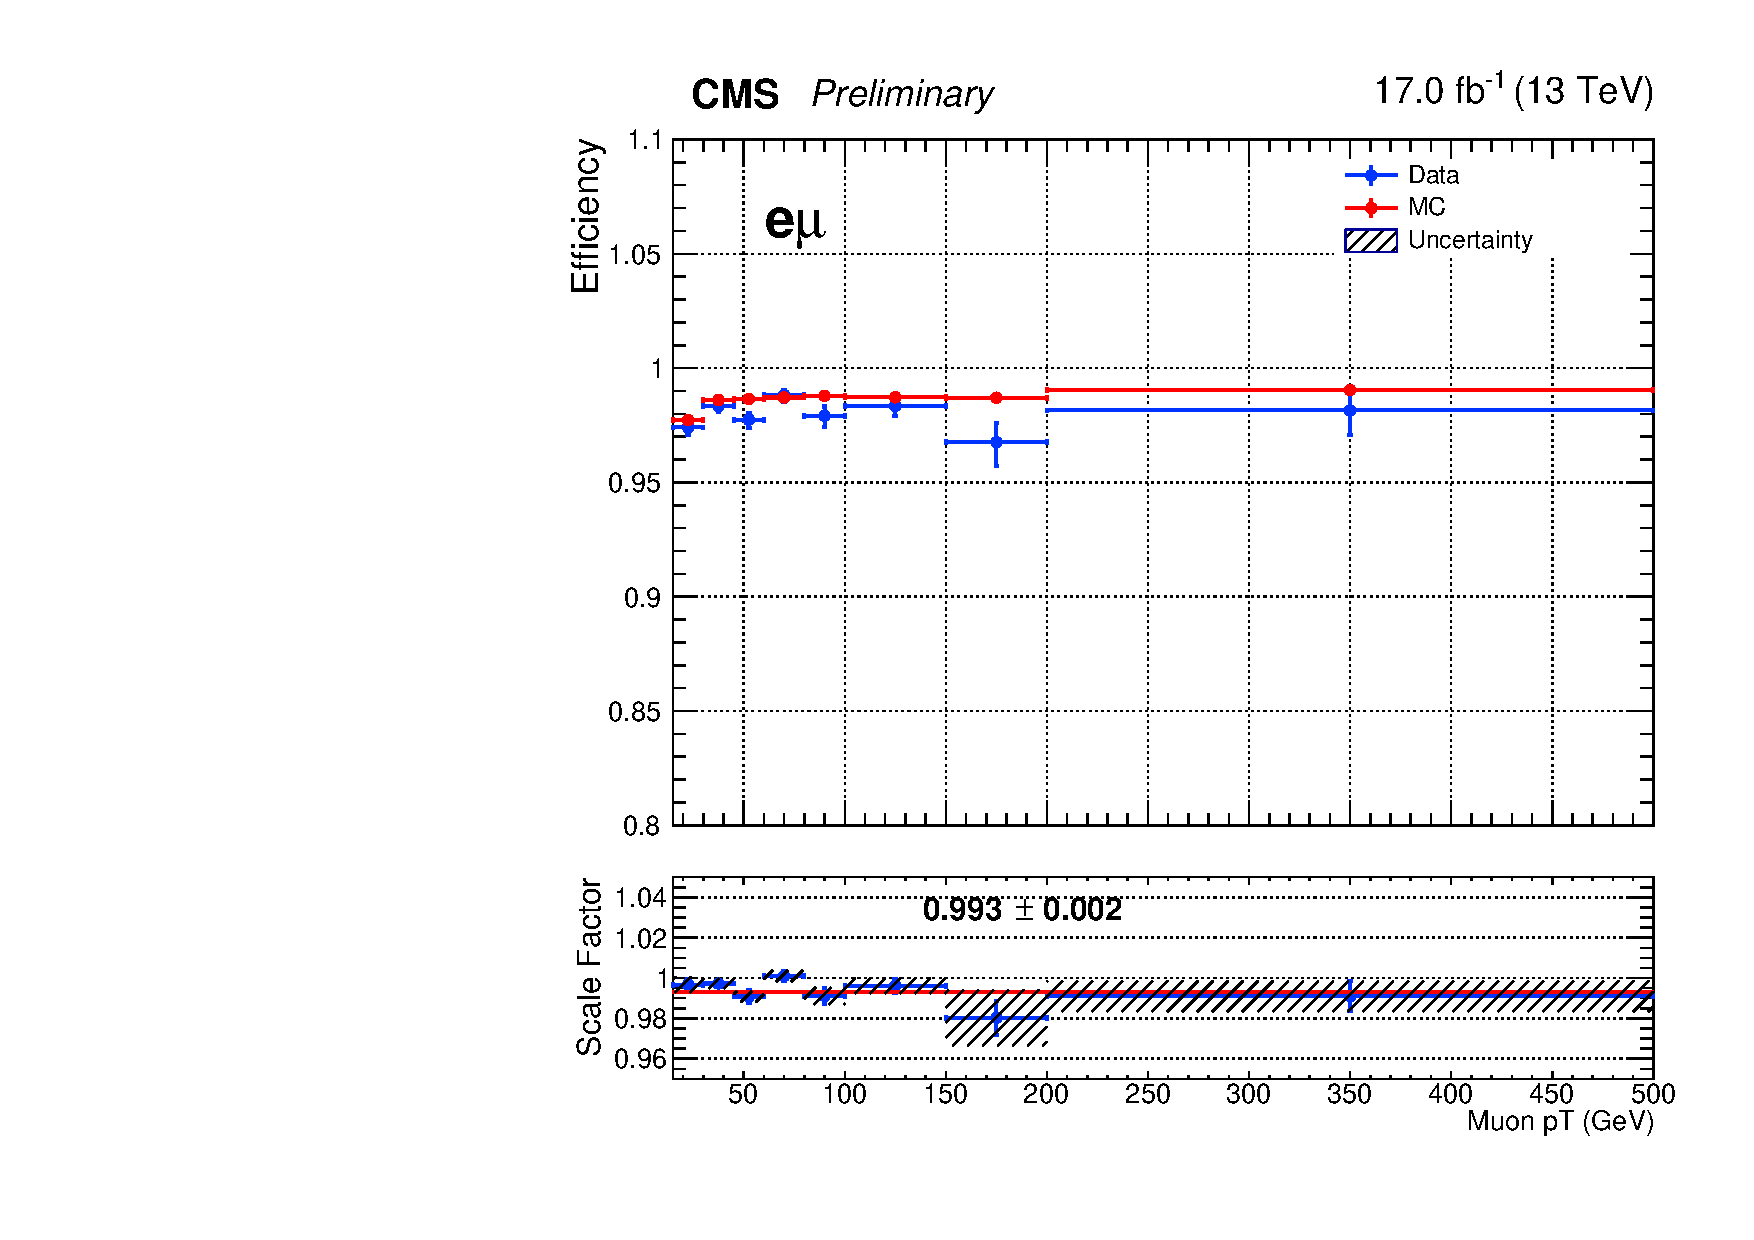
\includegraphics[width=0.32\textwidth]{fig_2016postVFP_TrigSF/g_emu_lepBpt_FullSystUncBand.pdf}\\
    \end{tabular}
    \caption{Efficiencies and scale factors for the 2016postVFP data set in the $e\mu$ channel as a function of electron and muon \pT.
            The error bars indicate the statistical uncertainty, and the shaded band corresponds to the systematic uncertainty.
            }
    \label{TrigSF_2016postVFP_1}
  \end{center}
\end{figure}

\begin{figure}[h]
  \begin{center}
    \begin{tabular}{ccc}
      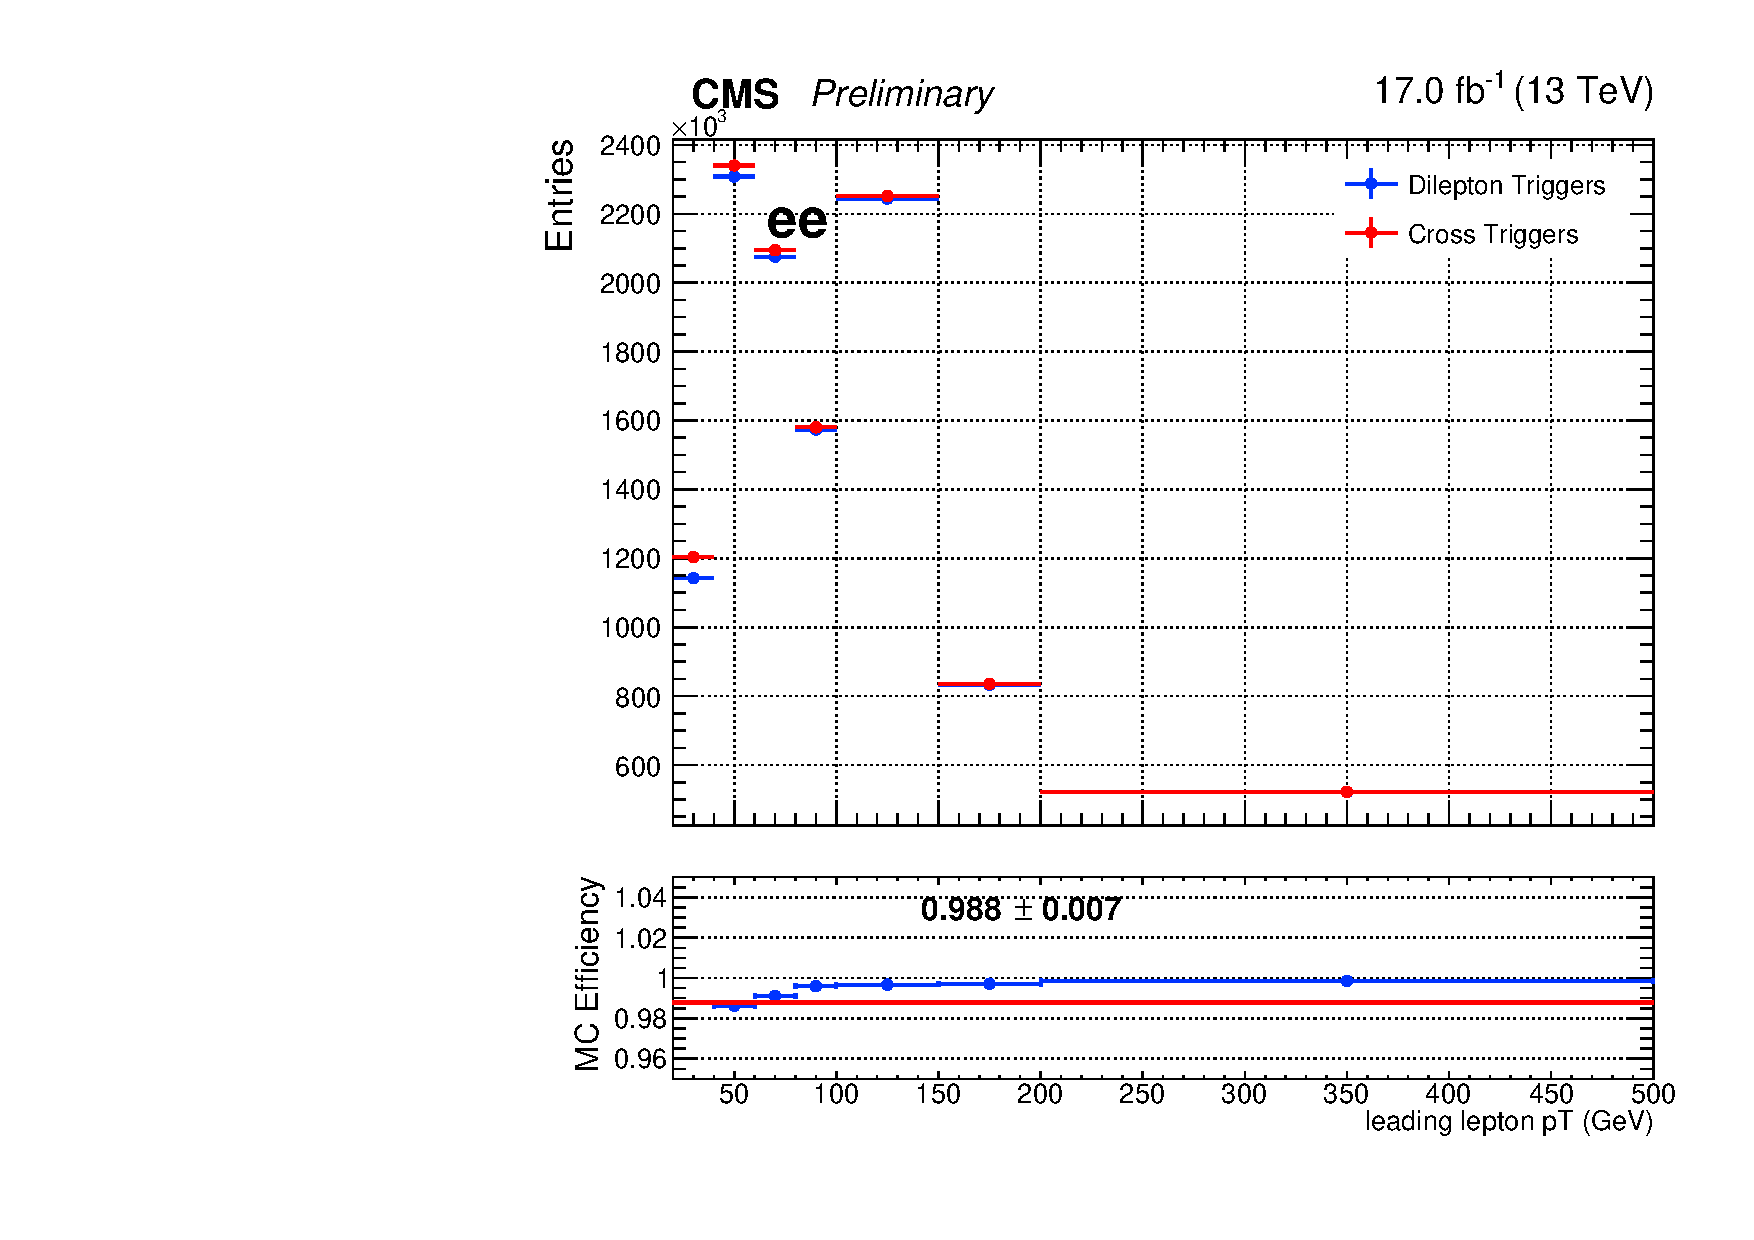
\includegraphics[width=0.32\textwidth]{fig_2016postVFP_TrigSF/g_lepApt_ee_MC.pdf}
      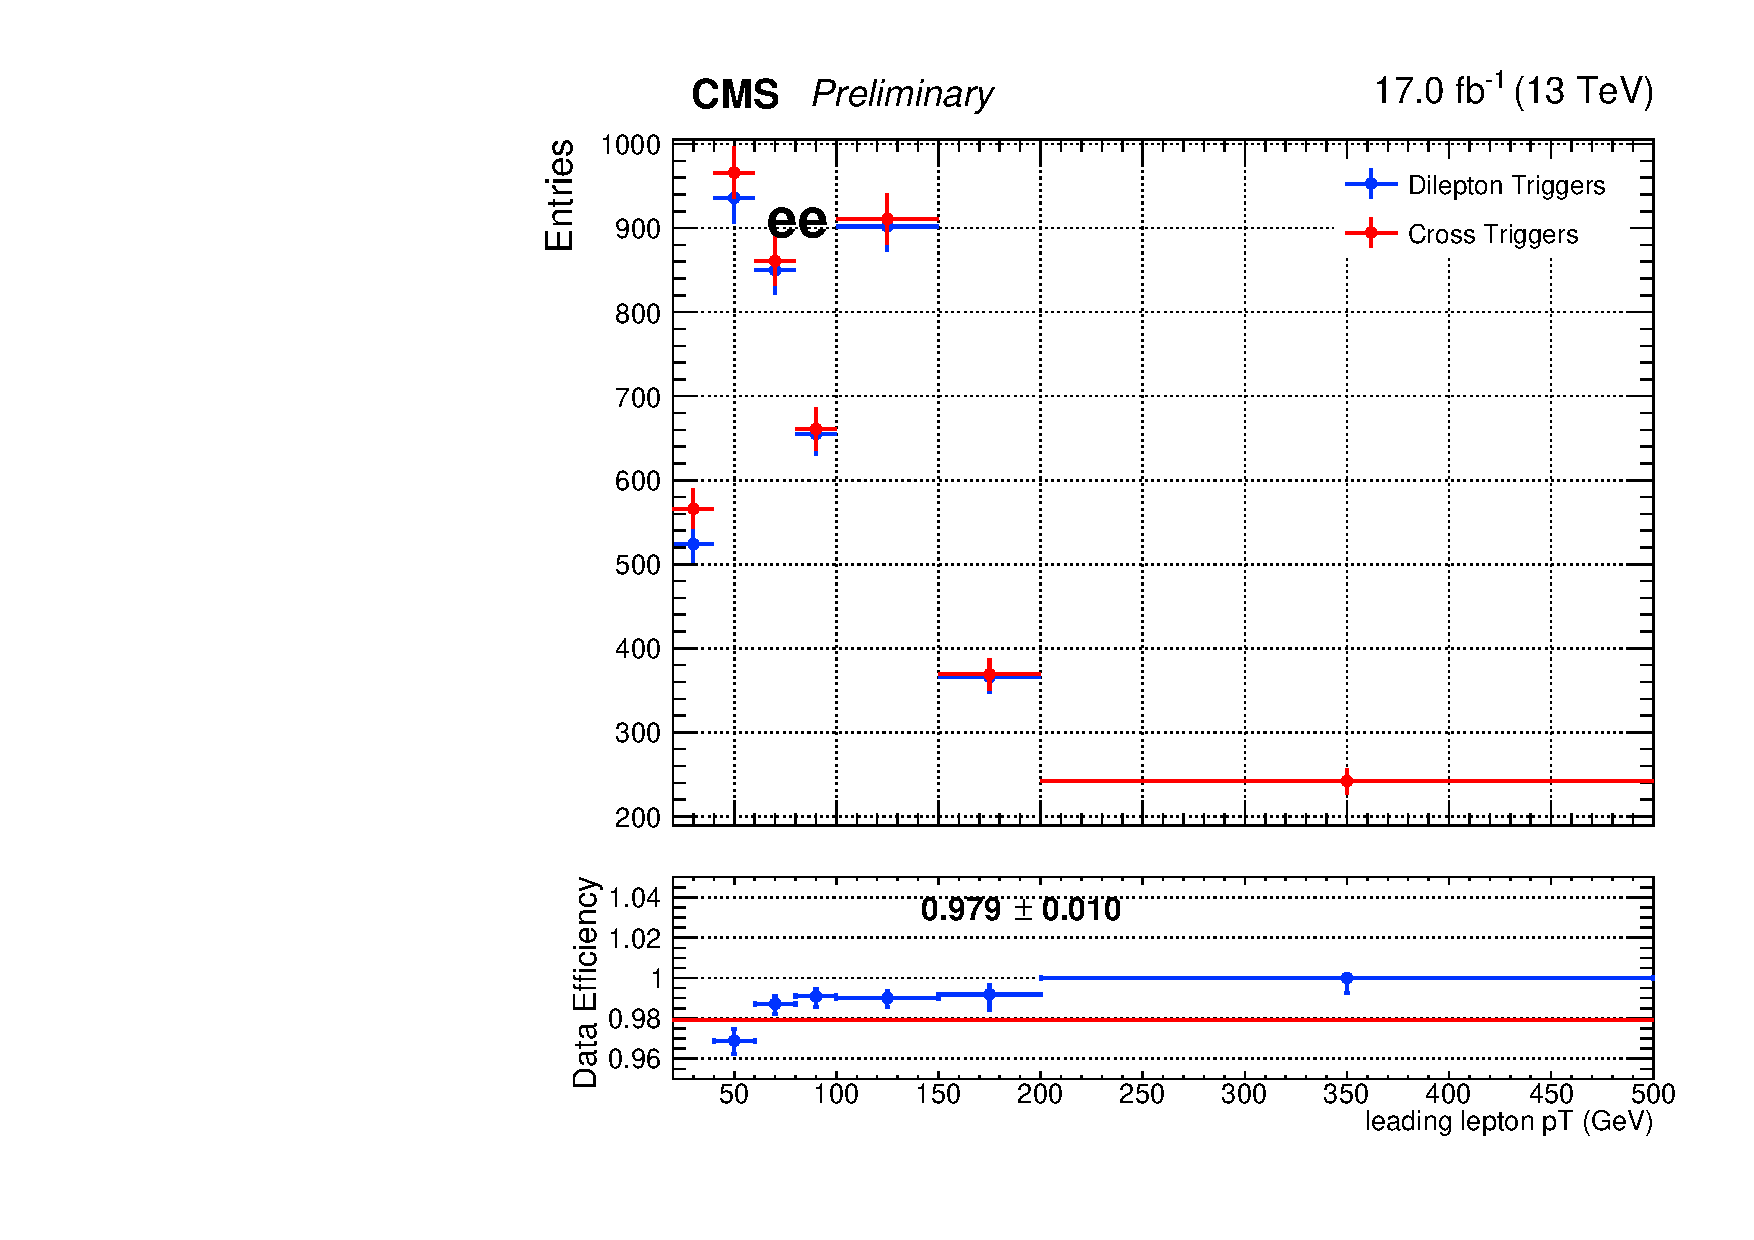
\includegraphics[width=0.32\textwidth]{fig_2016postVFP_TrigSF/g_lepApt_ee_data.pdf}
      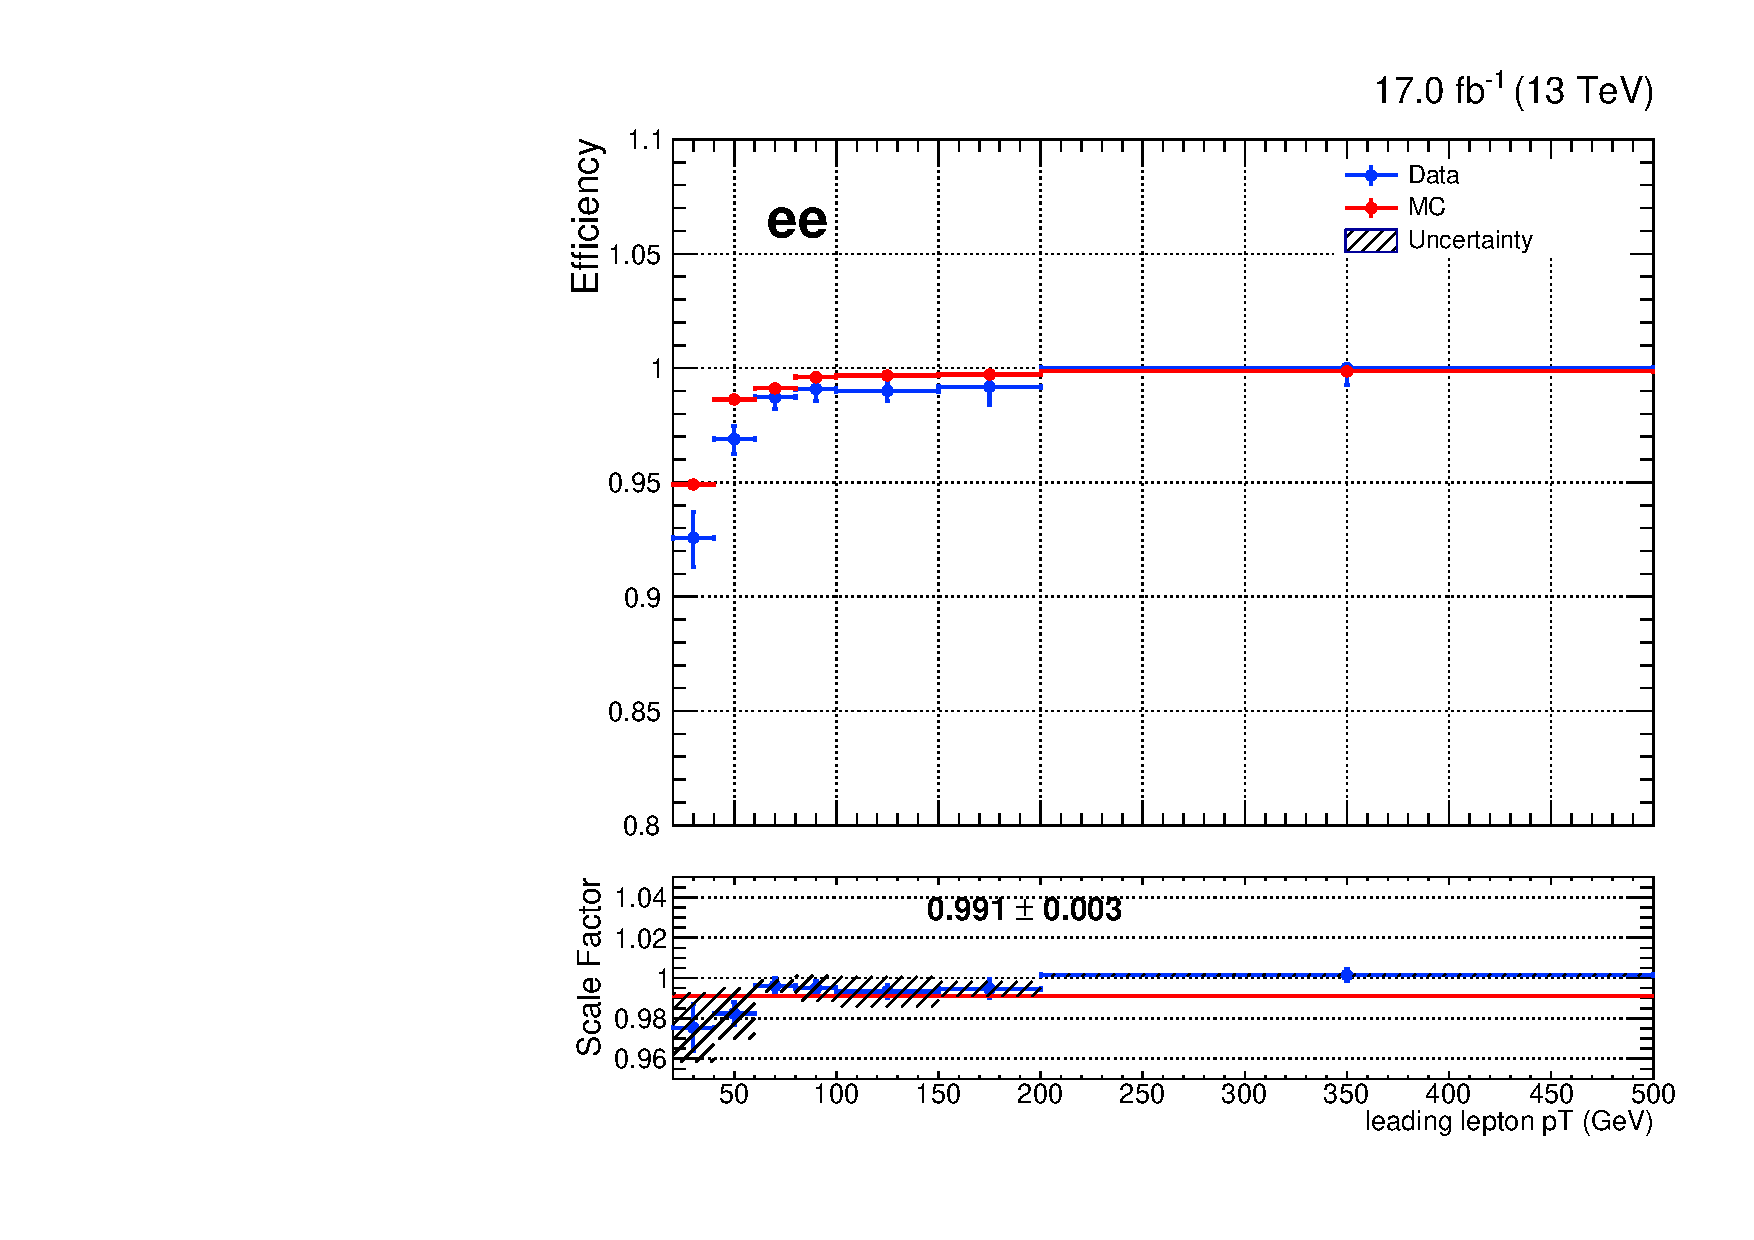
\includegraphics[width=0.32\textwidth]{fig_2016postVFP_TrigSF/g_ee_lepApt_FullSystUncBand.pdf}\\
      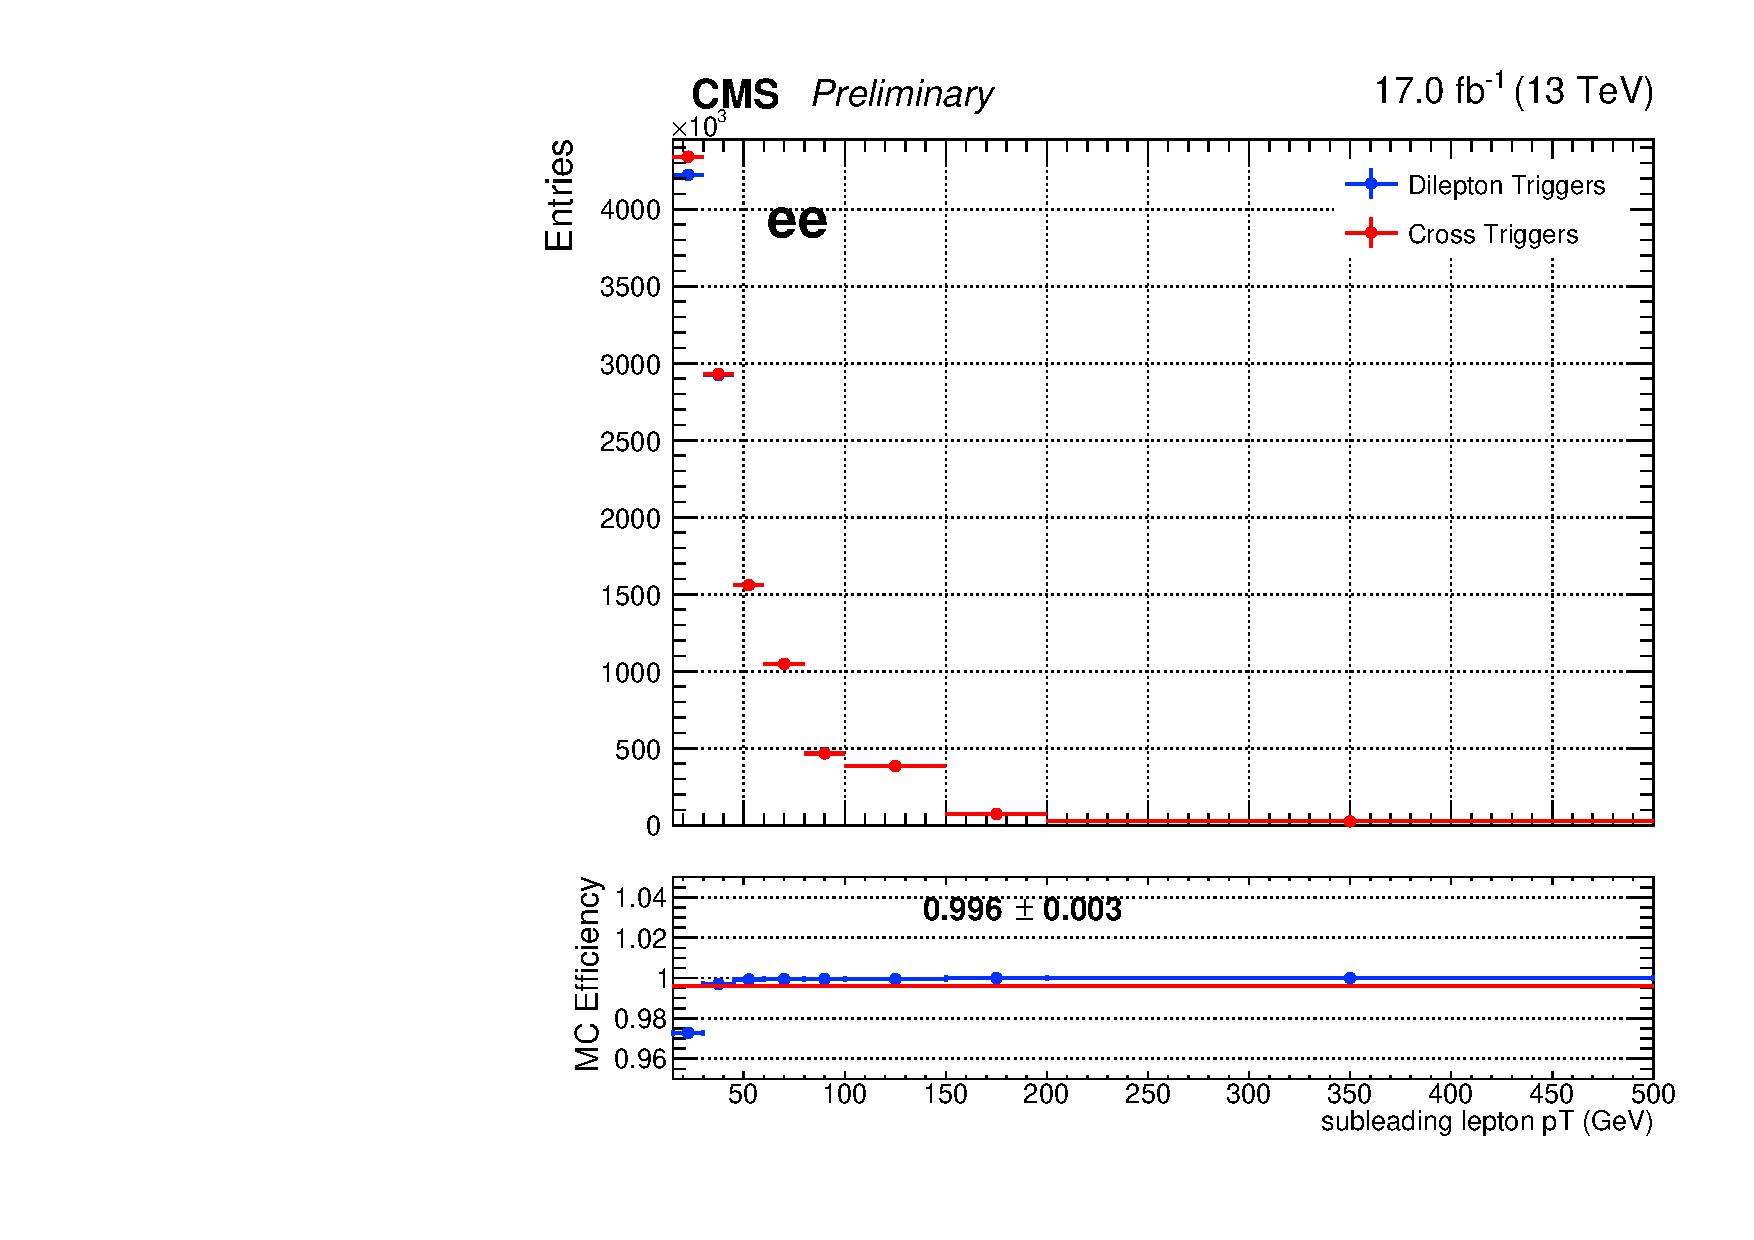
\includegraphics[width=0.32\textwidth]{fig_2016postVFP_TrigSF/g_lepBpt_ee_MC.pdf}
      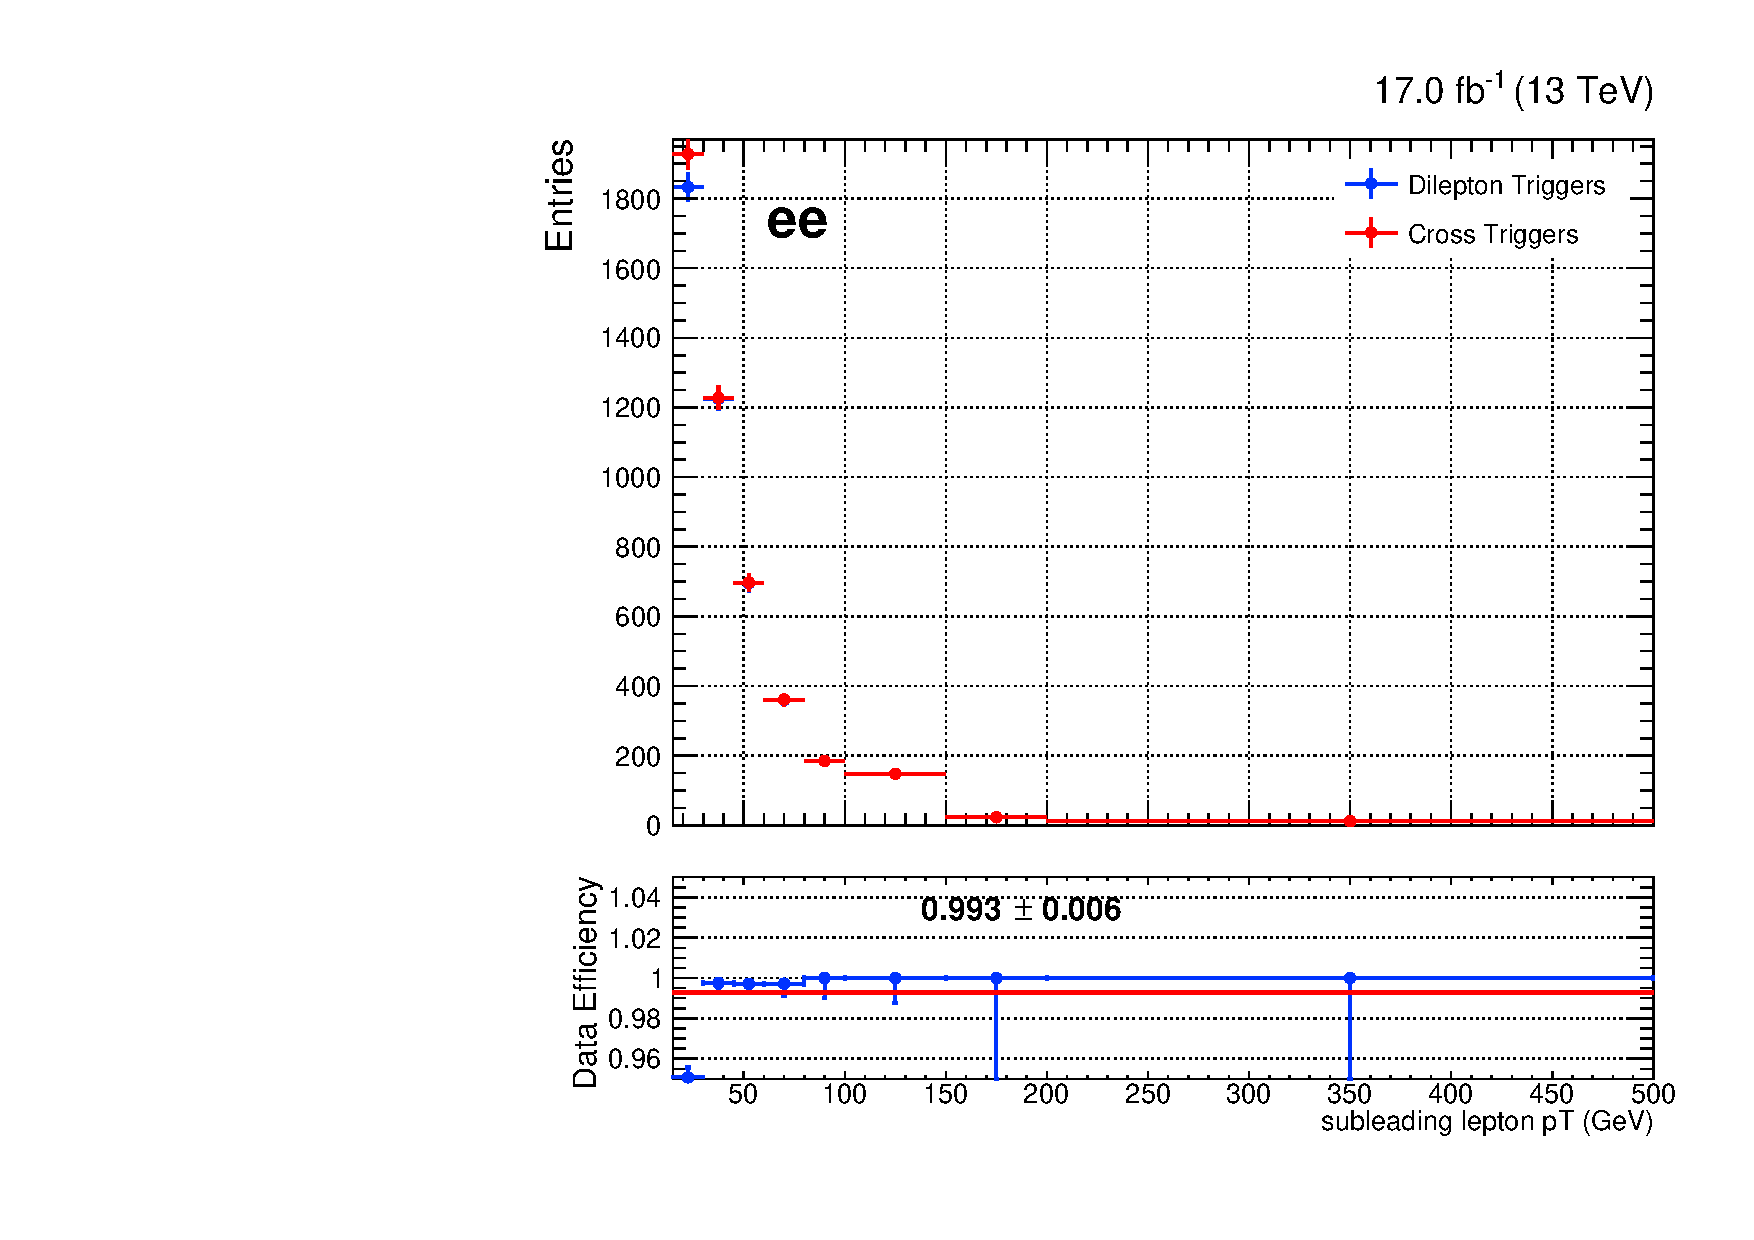
\includegraphics[width=0.32\textwidth]{fig_2016postVFP_TrigSF/g_lepBpt_ee_data.pdf}
      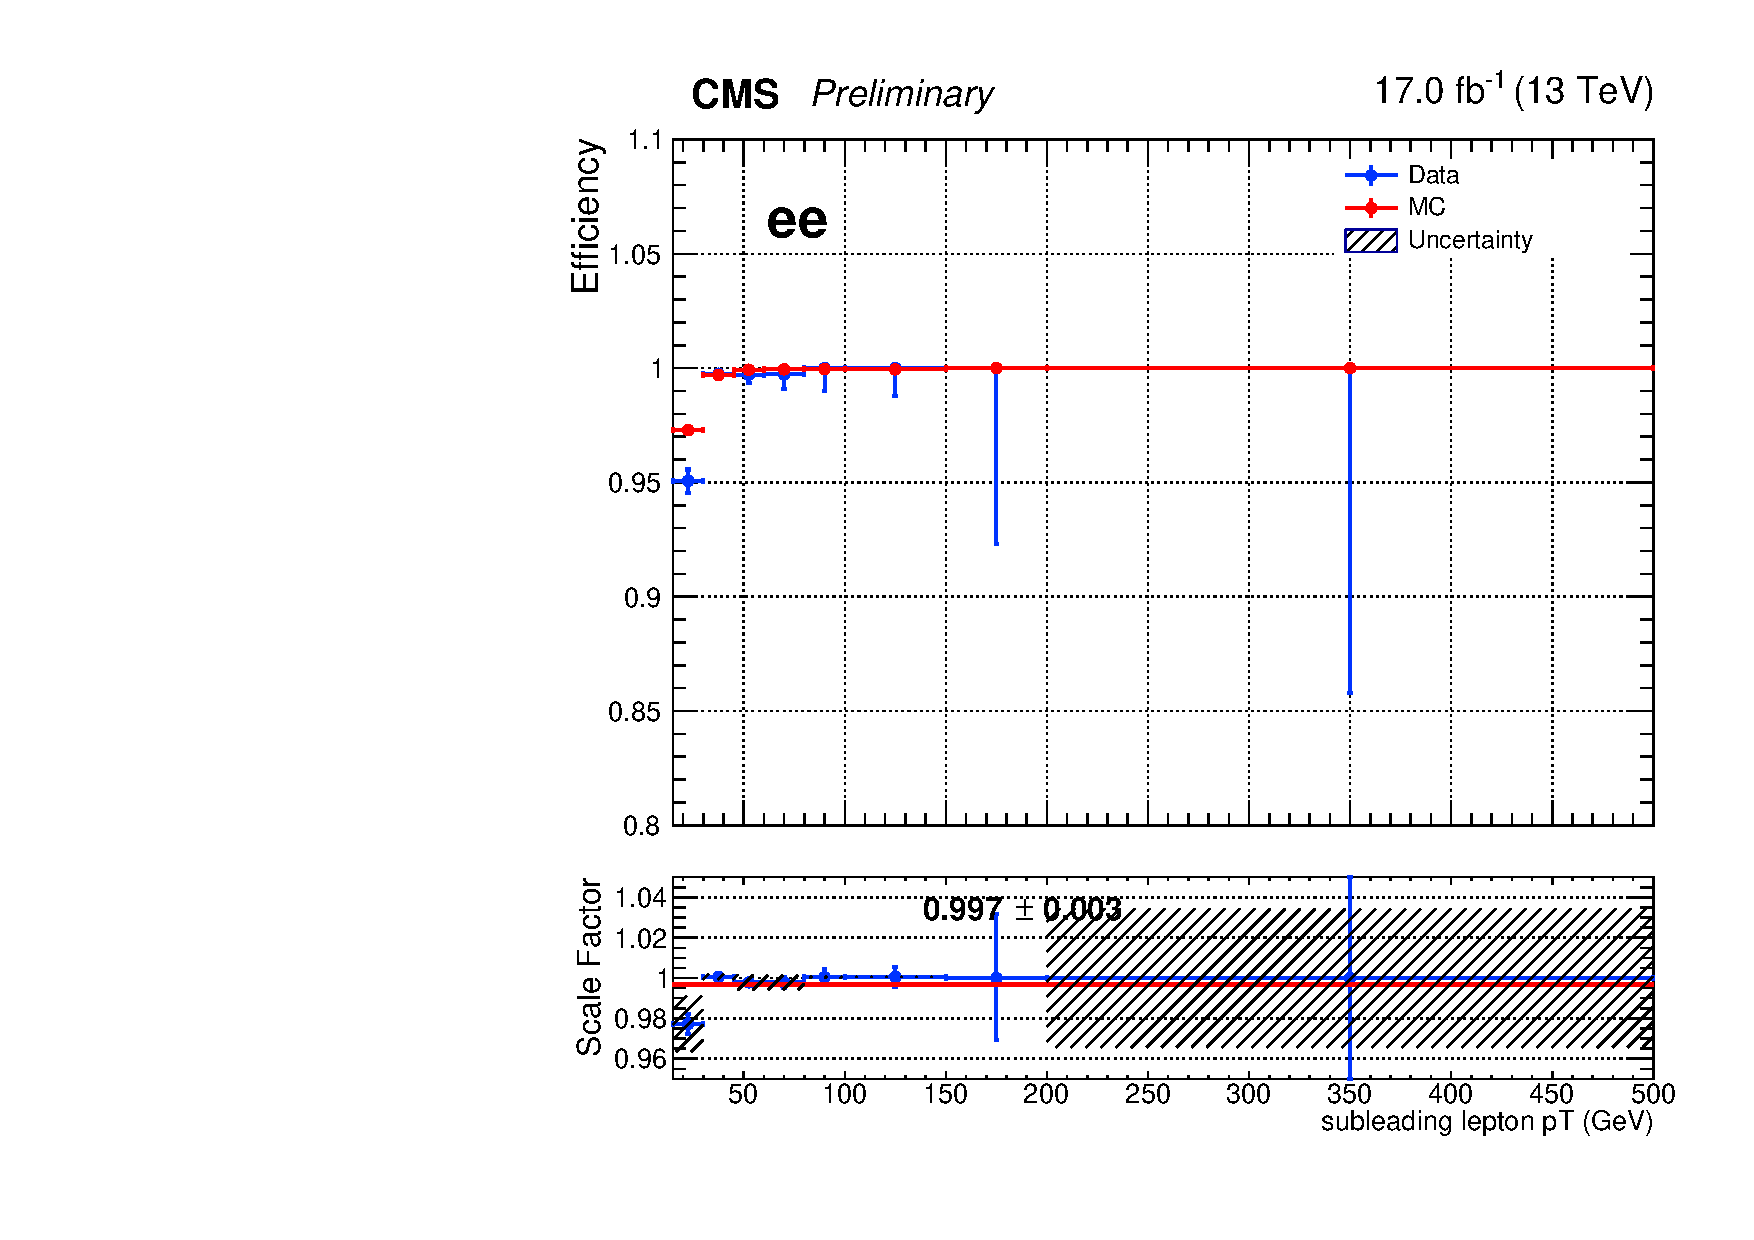
\includegraphics[width=0.32\textwidth]{fig_2016postVFP_TrigSF/g_ee_lepBpt_FullSystUncBand.pdf}\\
    \end{tabular}
    \caption{Efficiencies and scale factors for the 2016postVFP data set in the $ee$ channel as a function of leading and sub-leading lepton \pT.
            The error bars indicate the statistical uncertainty, and the shaded band corresponds to the systematic uncertainty.
            }
    \label{TrigSF_2016postVFP_2}
  \end{center}
\end{figure}

\begin{figure}[h]
  \begin{center}
    \begin{tabular}{ccc}
      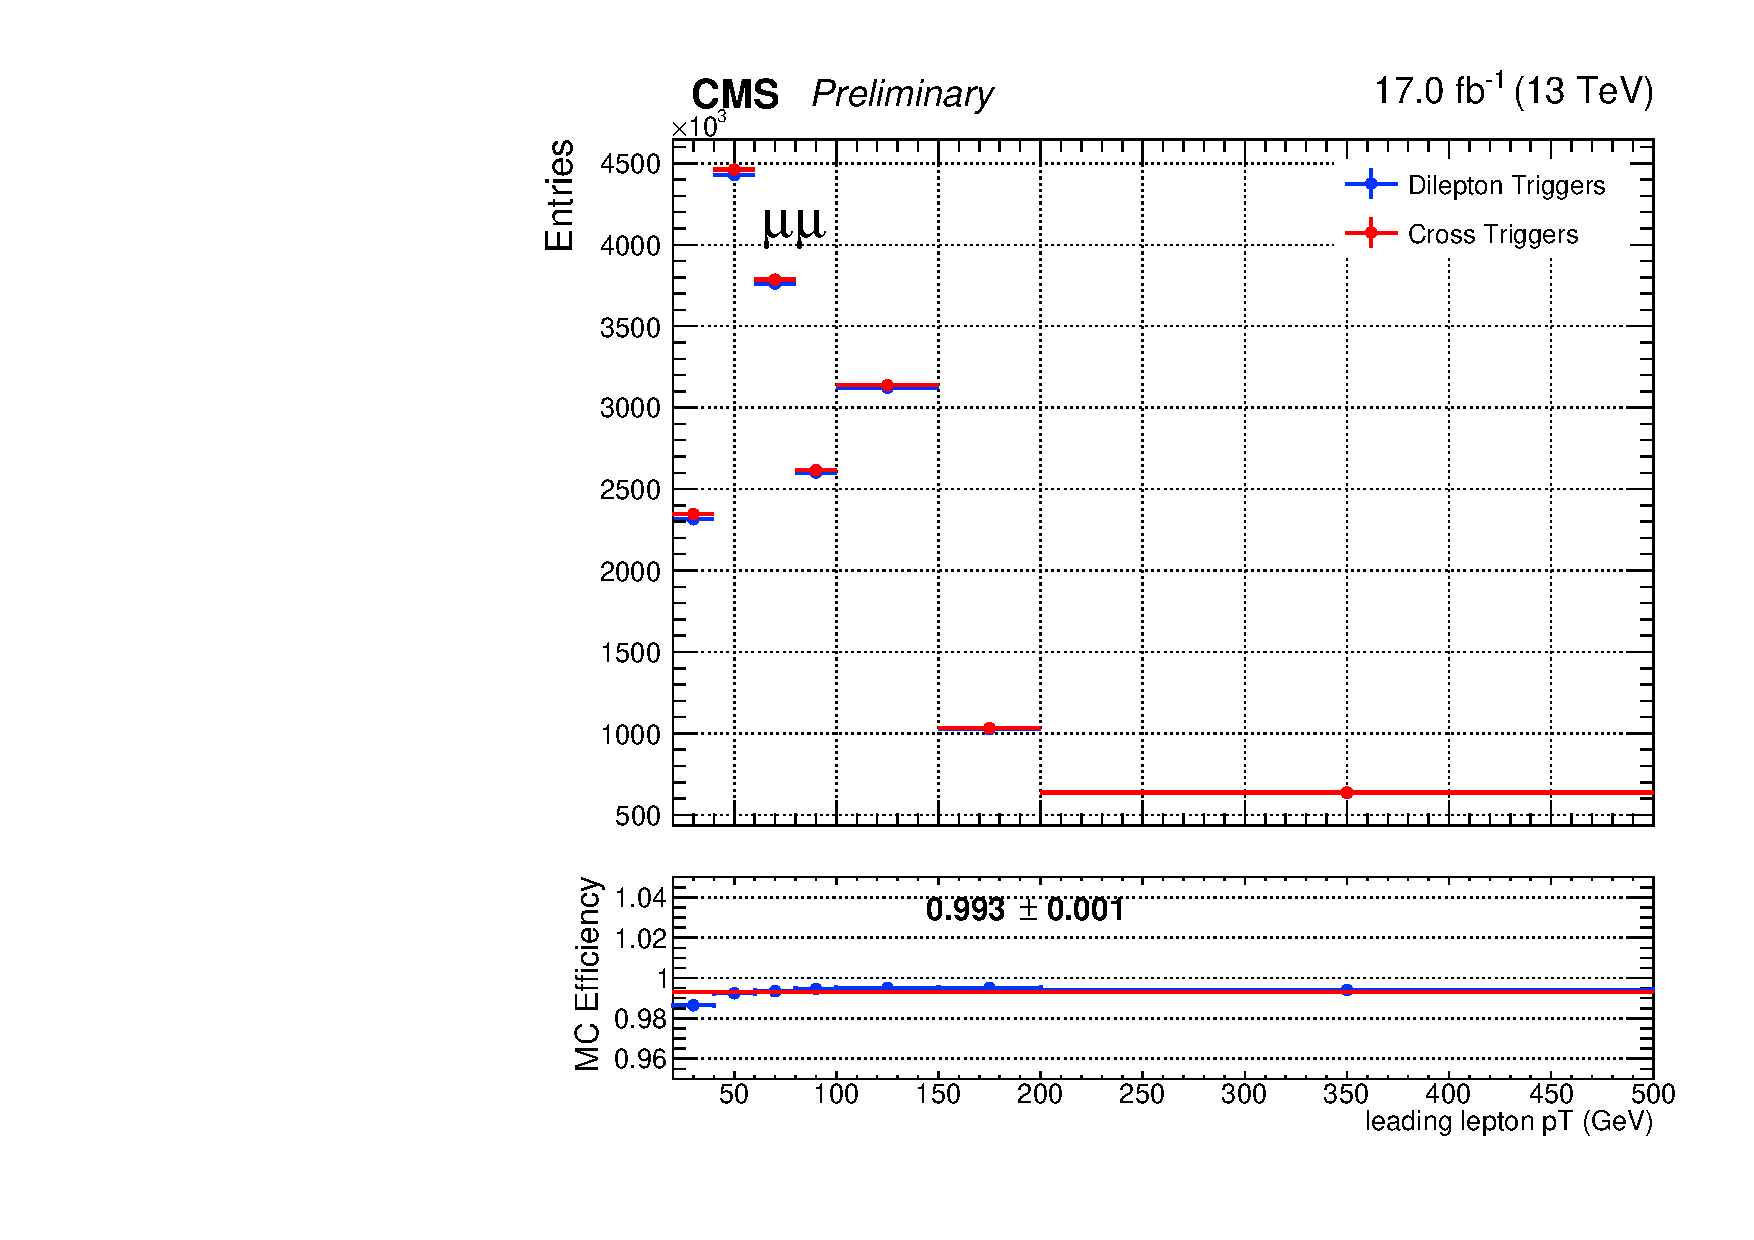
\includegraphics[width=0.32\textwidth]{fig_2016postVFP_TrigSF/g_lepApt_mumu_MC.pdf}
      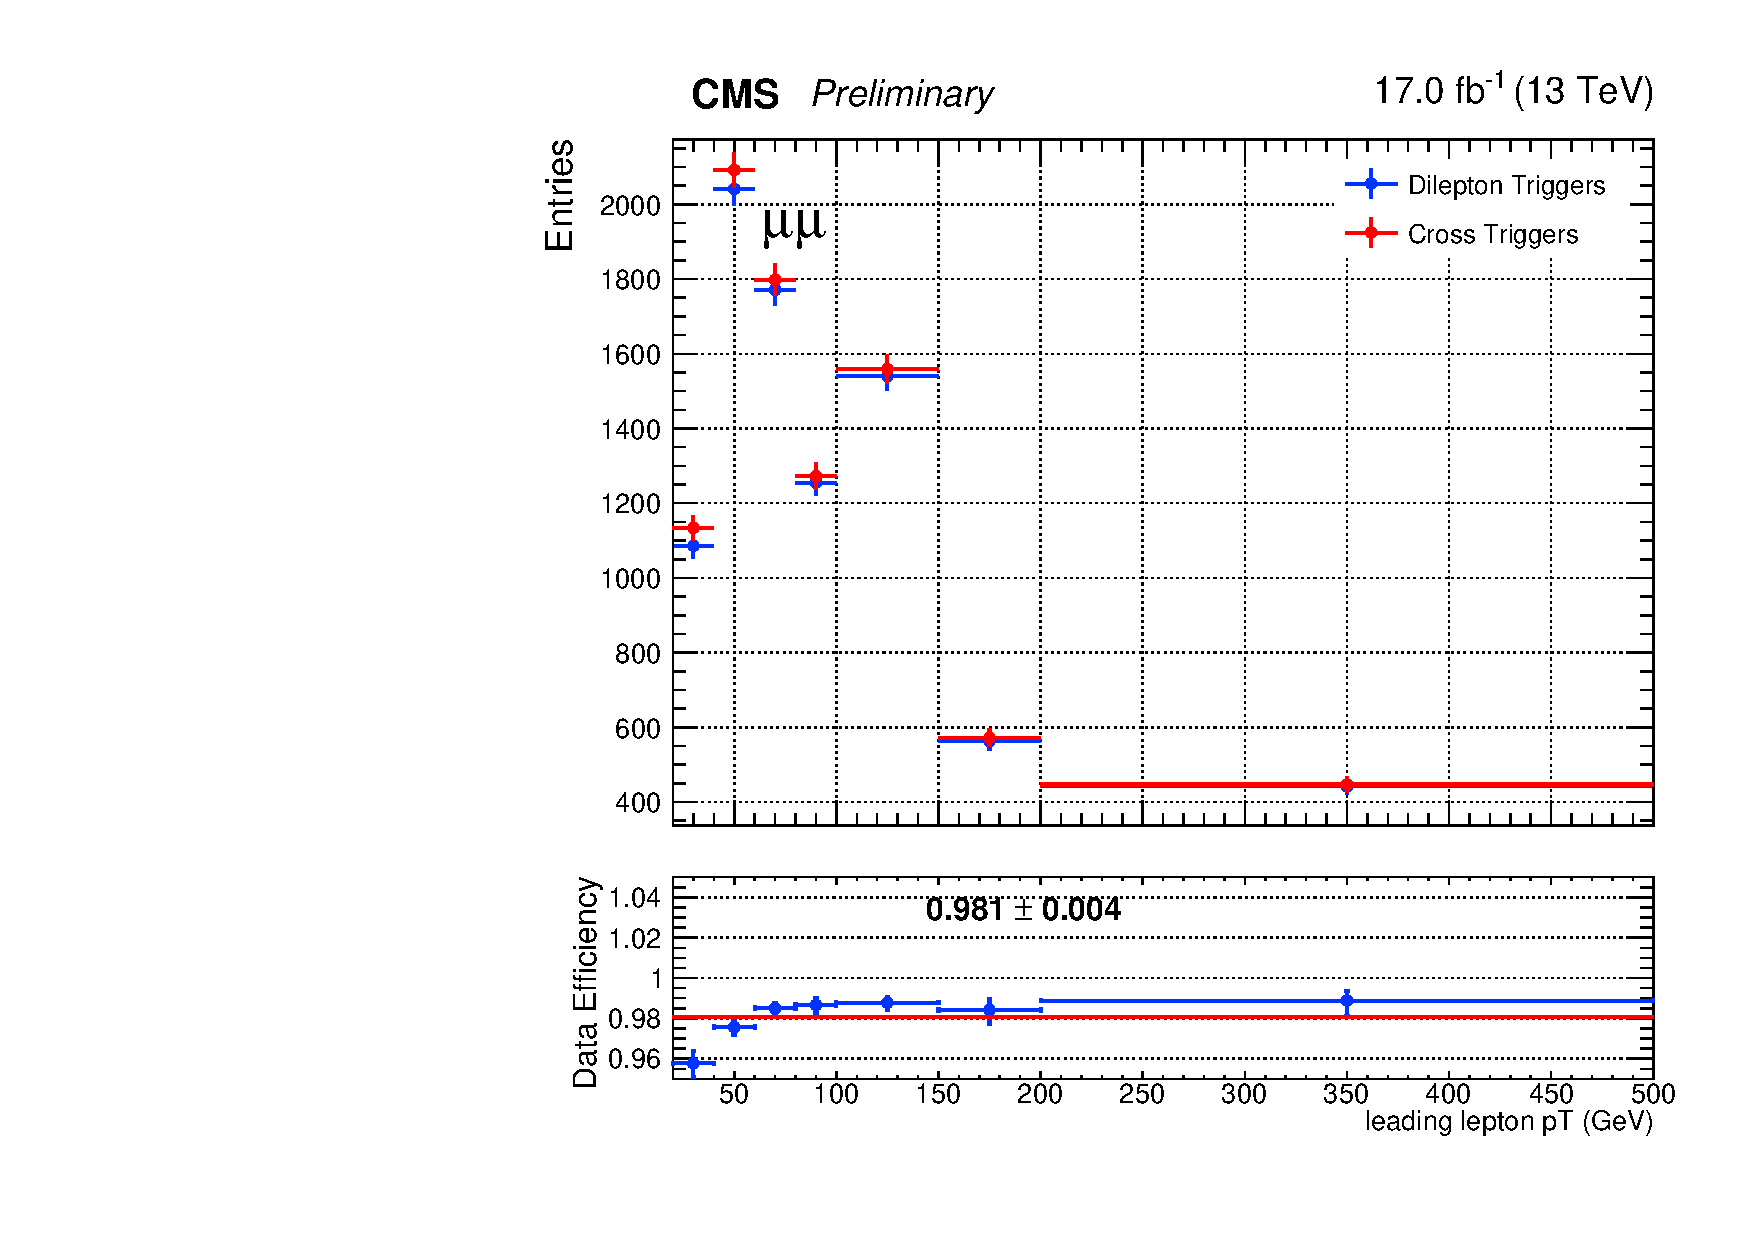
\includegraphics[width=0.32\textwidth]{fig_2016postVFP_TrigSF/g_lepApt_mumu_data.pdf}
      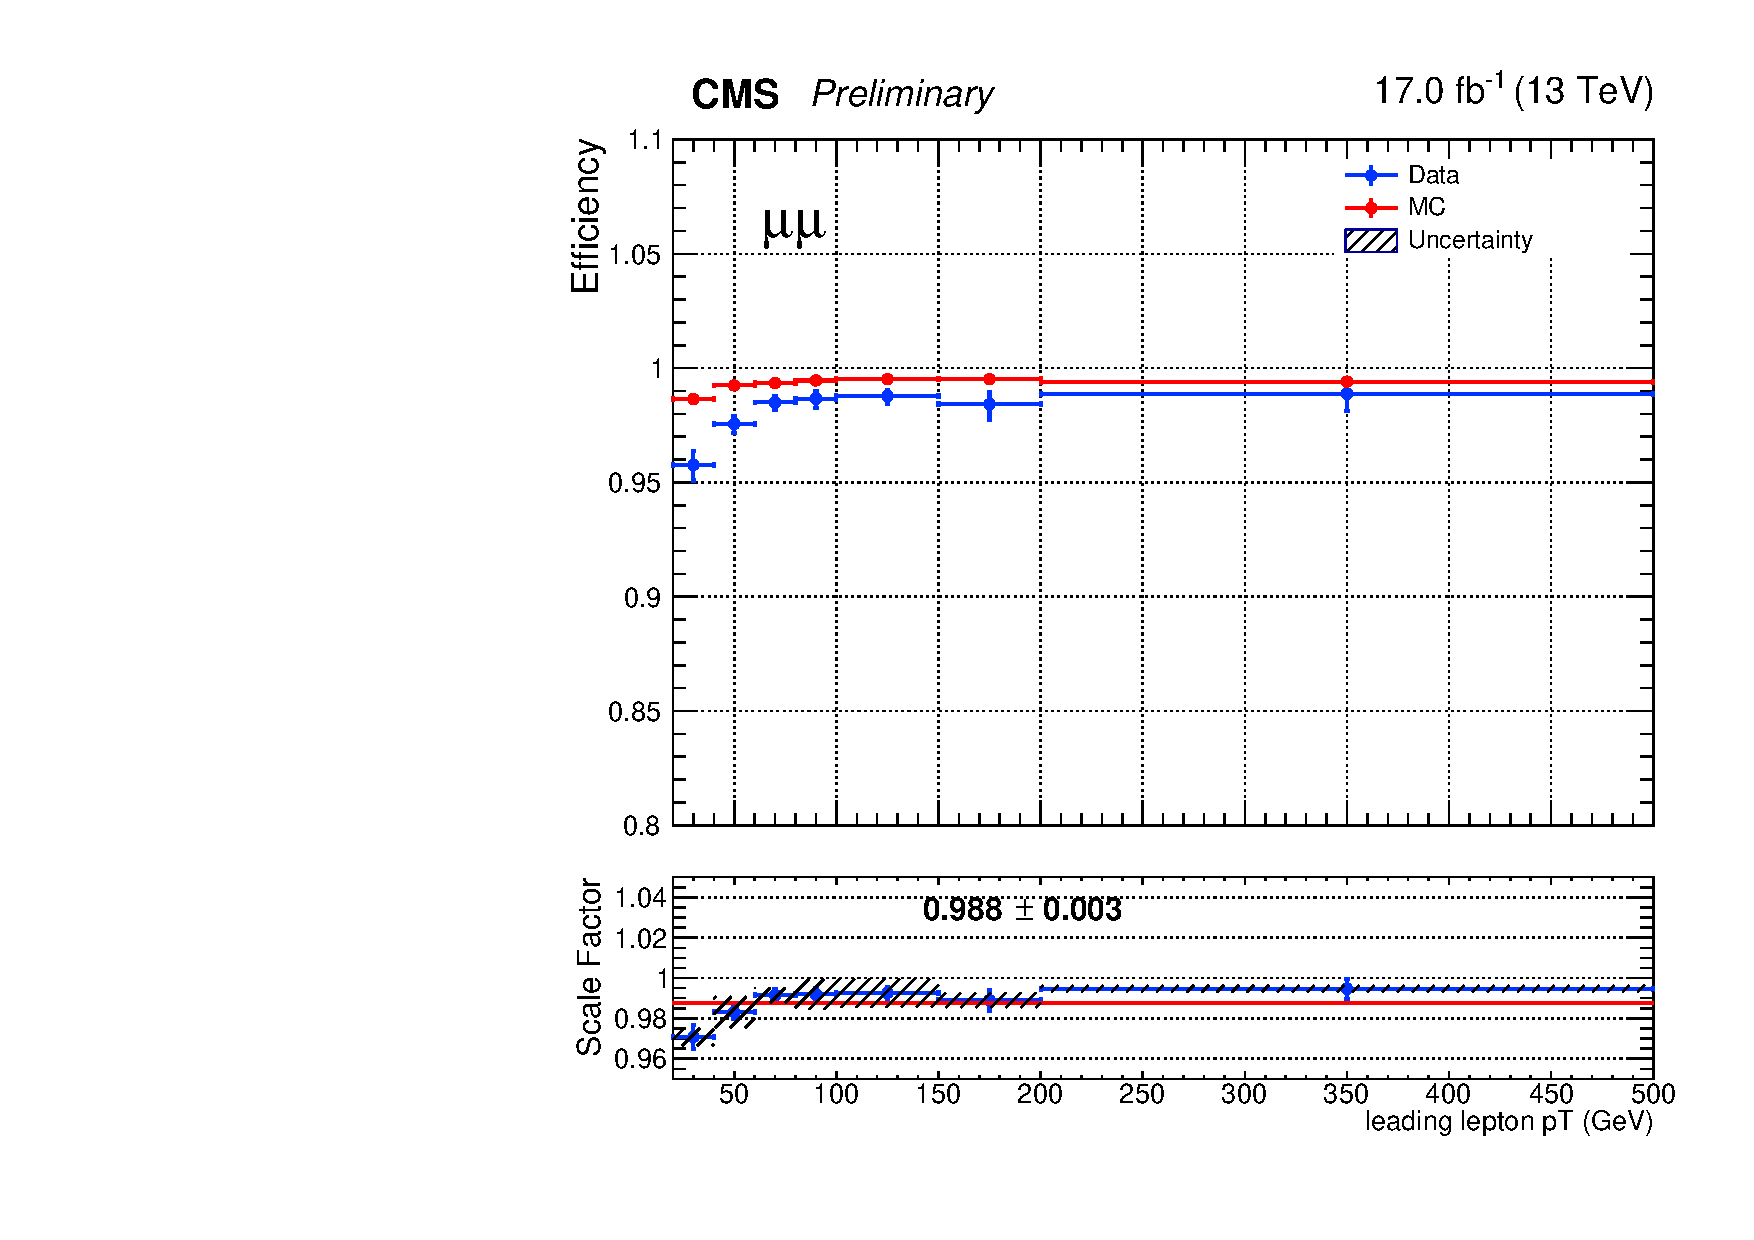
\includegraphics[width=0.32\textwidth]{fig_2016postVFP_TrigSF/g_mumu_lepApt_FullSystUncBand.pdf}\\
      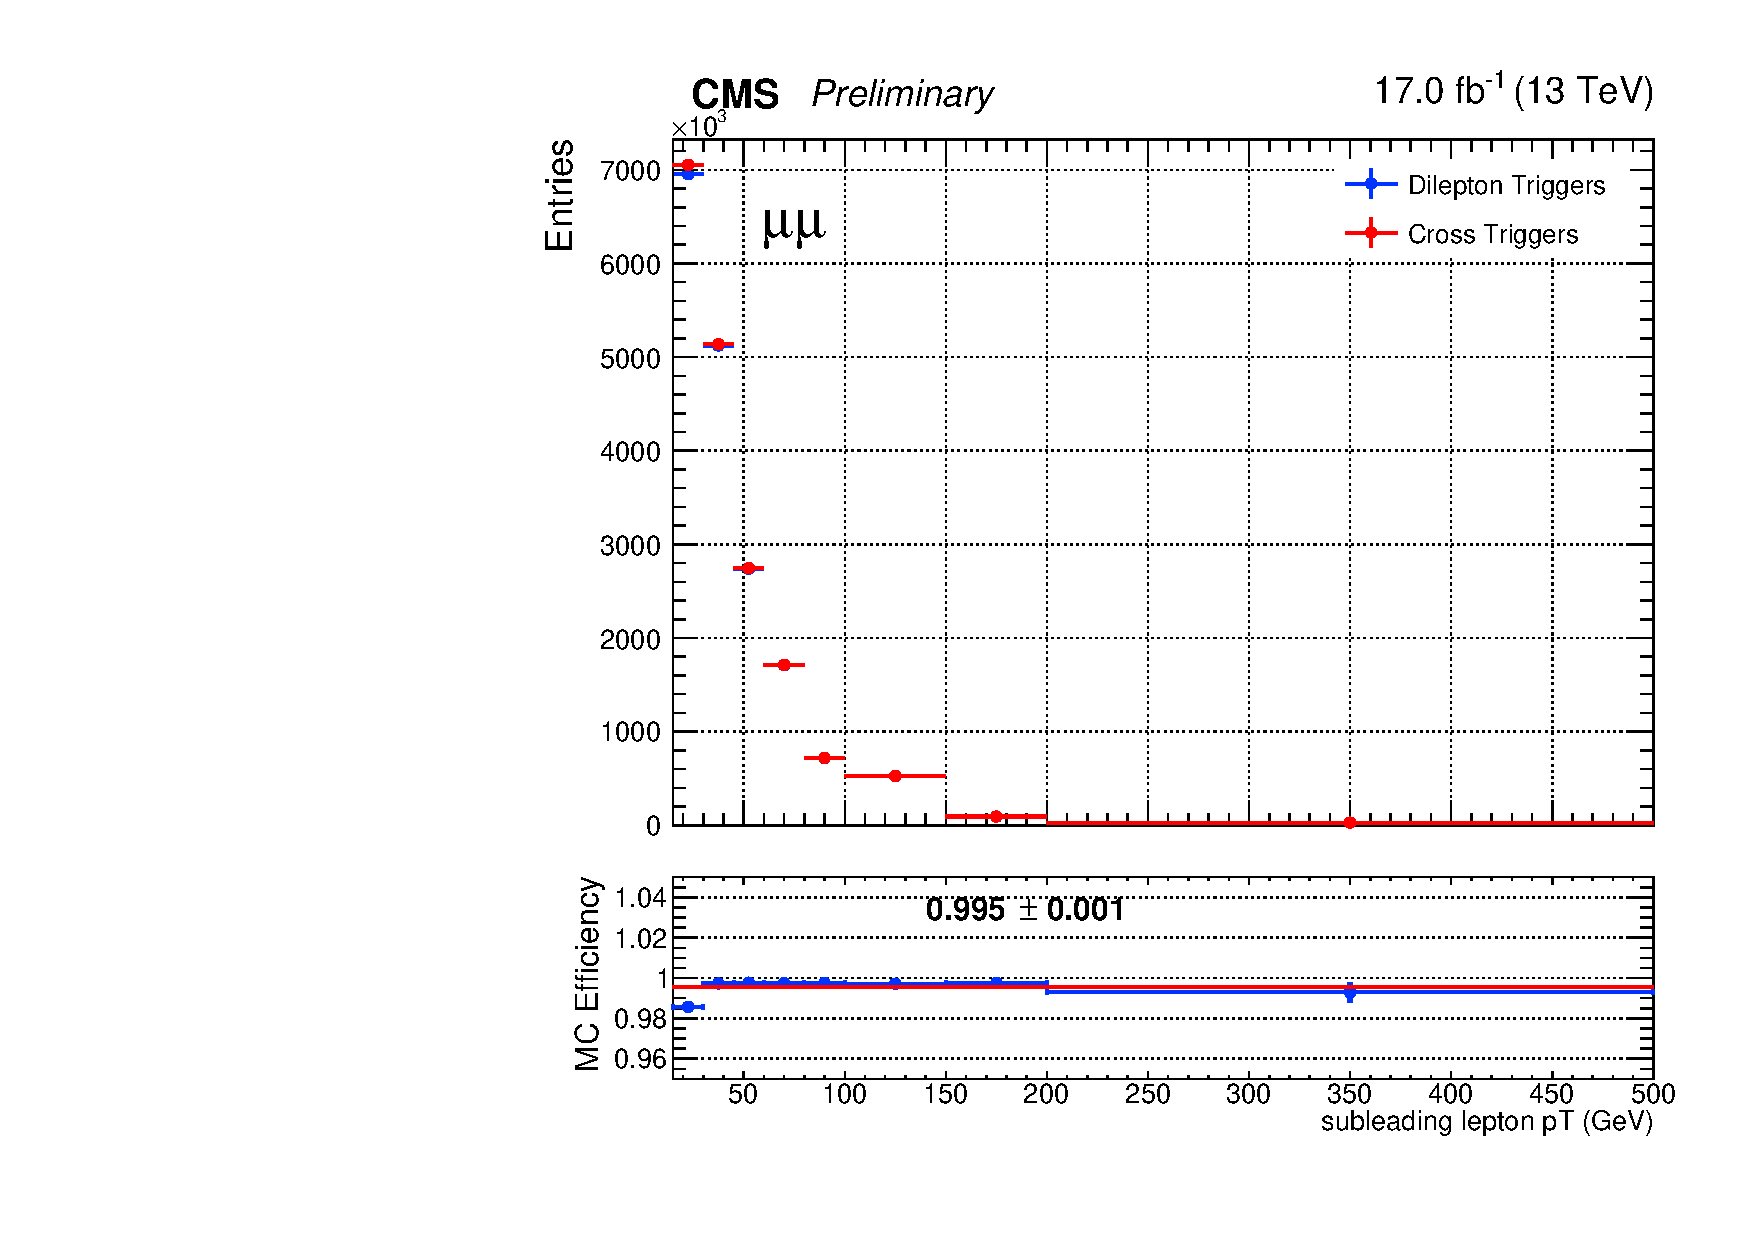
\includegraphics[width=0.32\textwidth]{fig_2016postVFP_TrigSF/g_lepBpt_mumu_MC.pdf}
      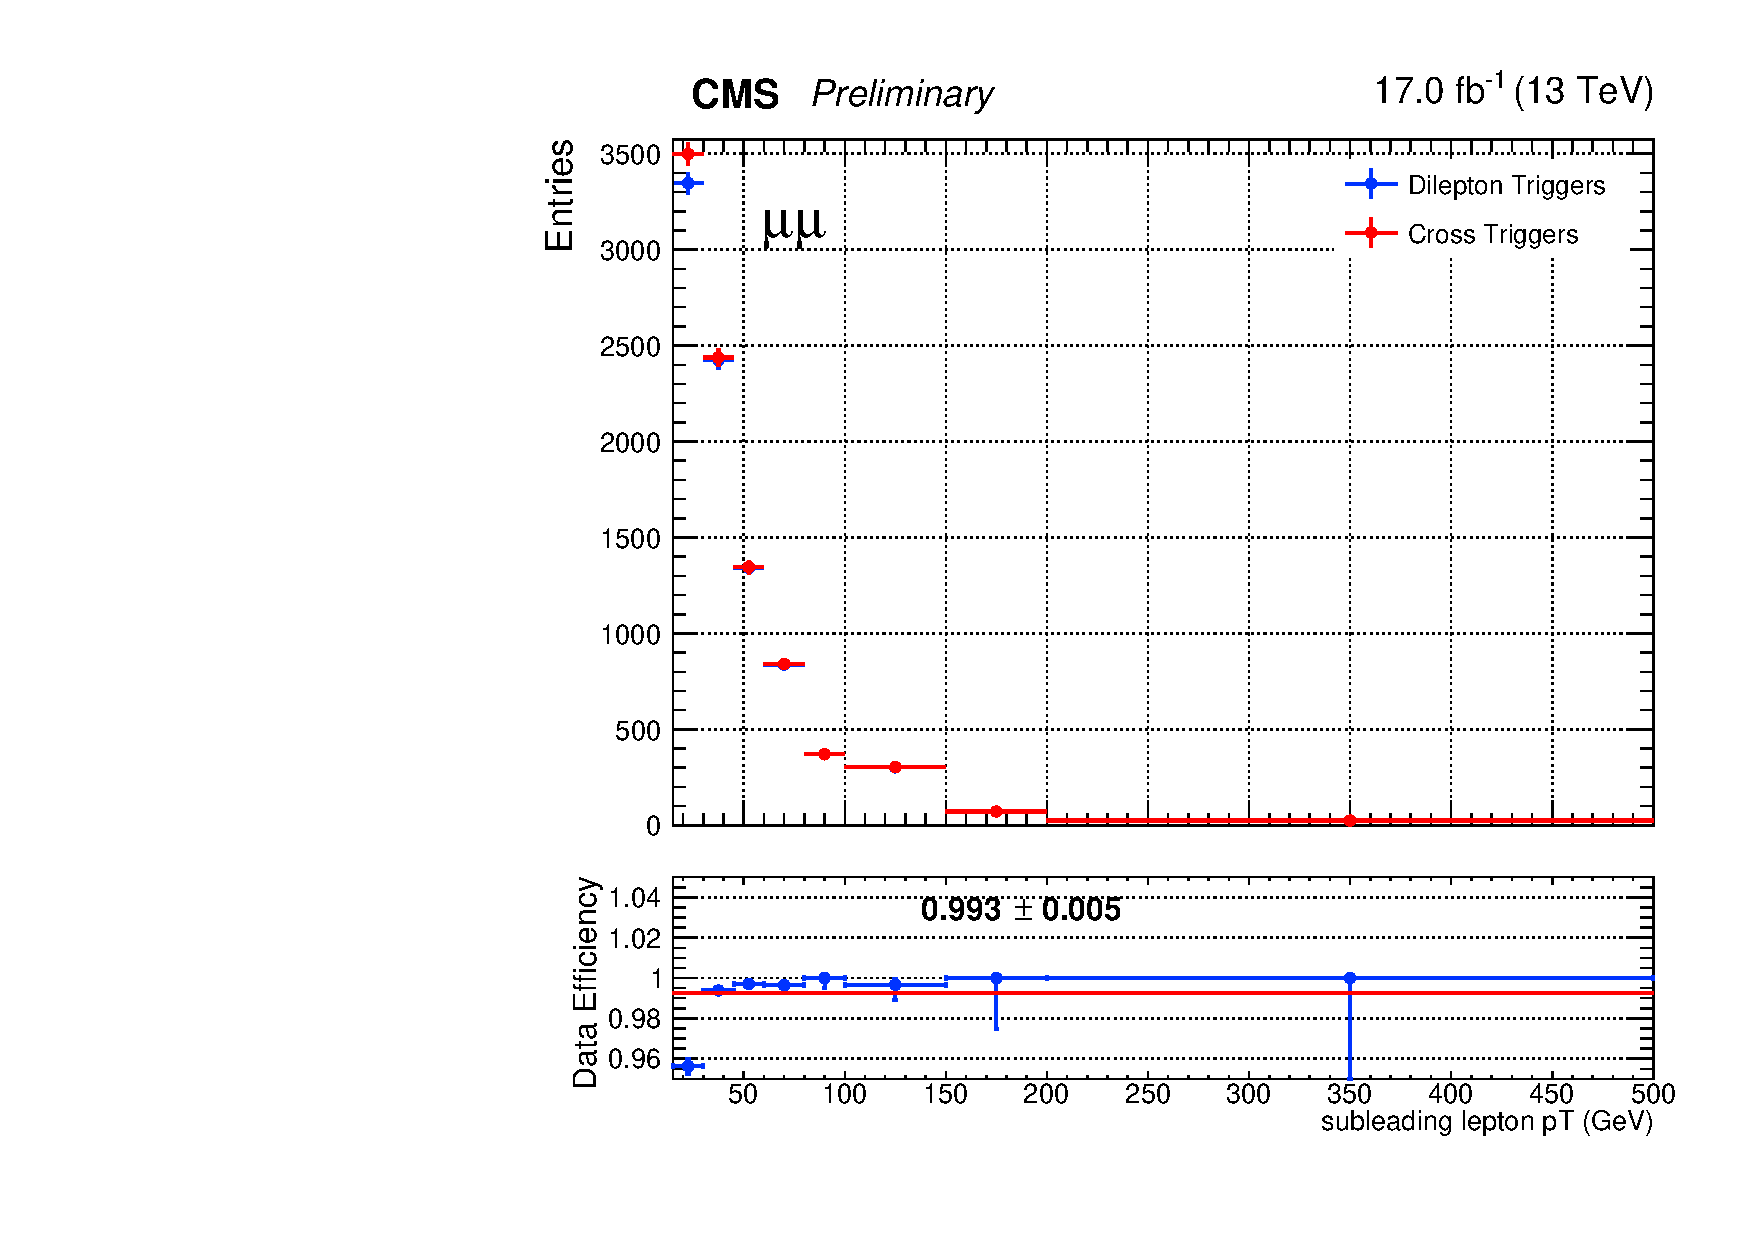
\includegraphics[width=0.32\textwidth]{fig_2016postVFP_TrigSF/g_lepBpt_mumu_data.pdf}
      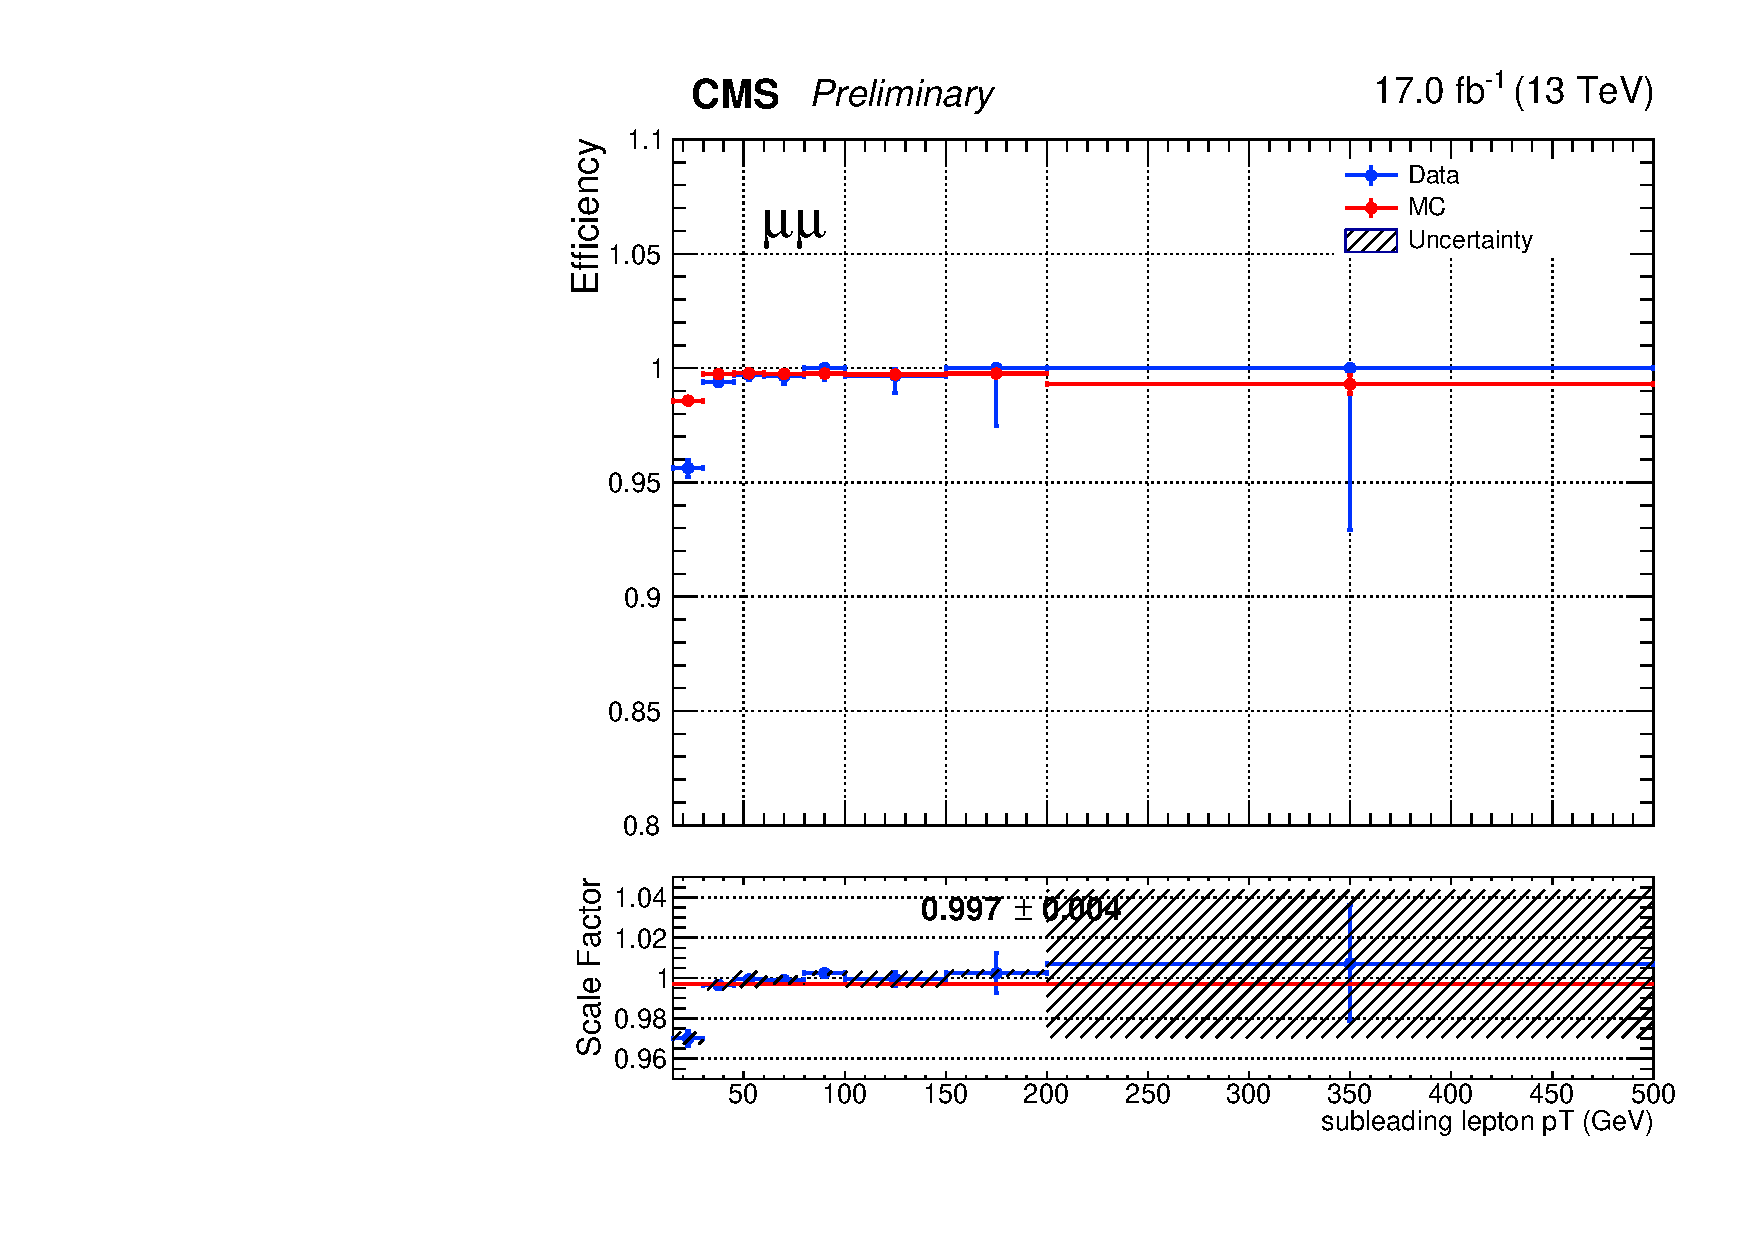
\includegraphics[width=0.32\textwidth]{fig_2016postVFP_TrigSF/g_mumu_lepBpt_FullSystUncBand.pdf}\\
    \end{tabular}
    \caption{Efficiencies and scale factors for the 2016postVFP data set in the $\mu\mu$ channel as a function of leading and sub-leading lepton \pT.
            The error bars indicate the statistical uncertainty, and the shaded band corresponds to the systematic uncertainty.
            }
    \label{TrigSF_2016postVFP_3}
  \end{center}
\end{figure}

\begin{figure}[h]
  \begin{center}
    \begin{tabular}{cc}
      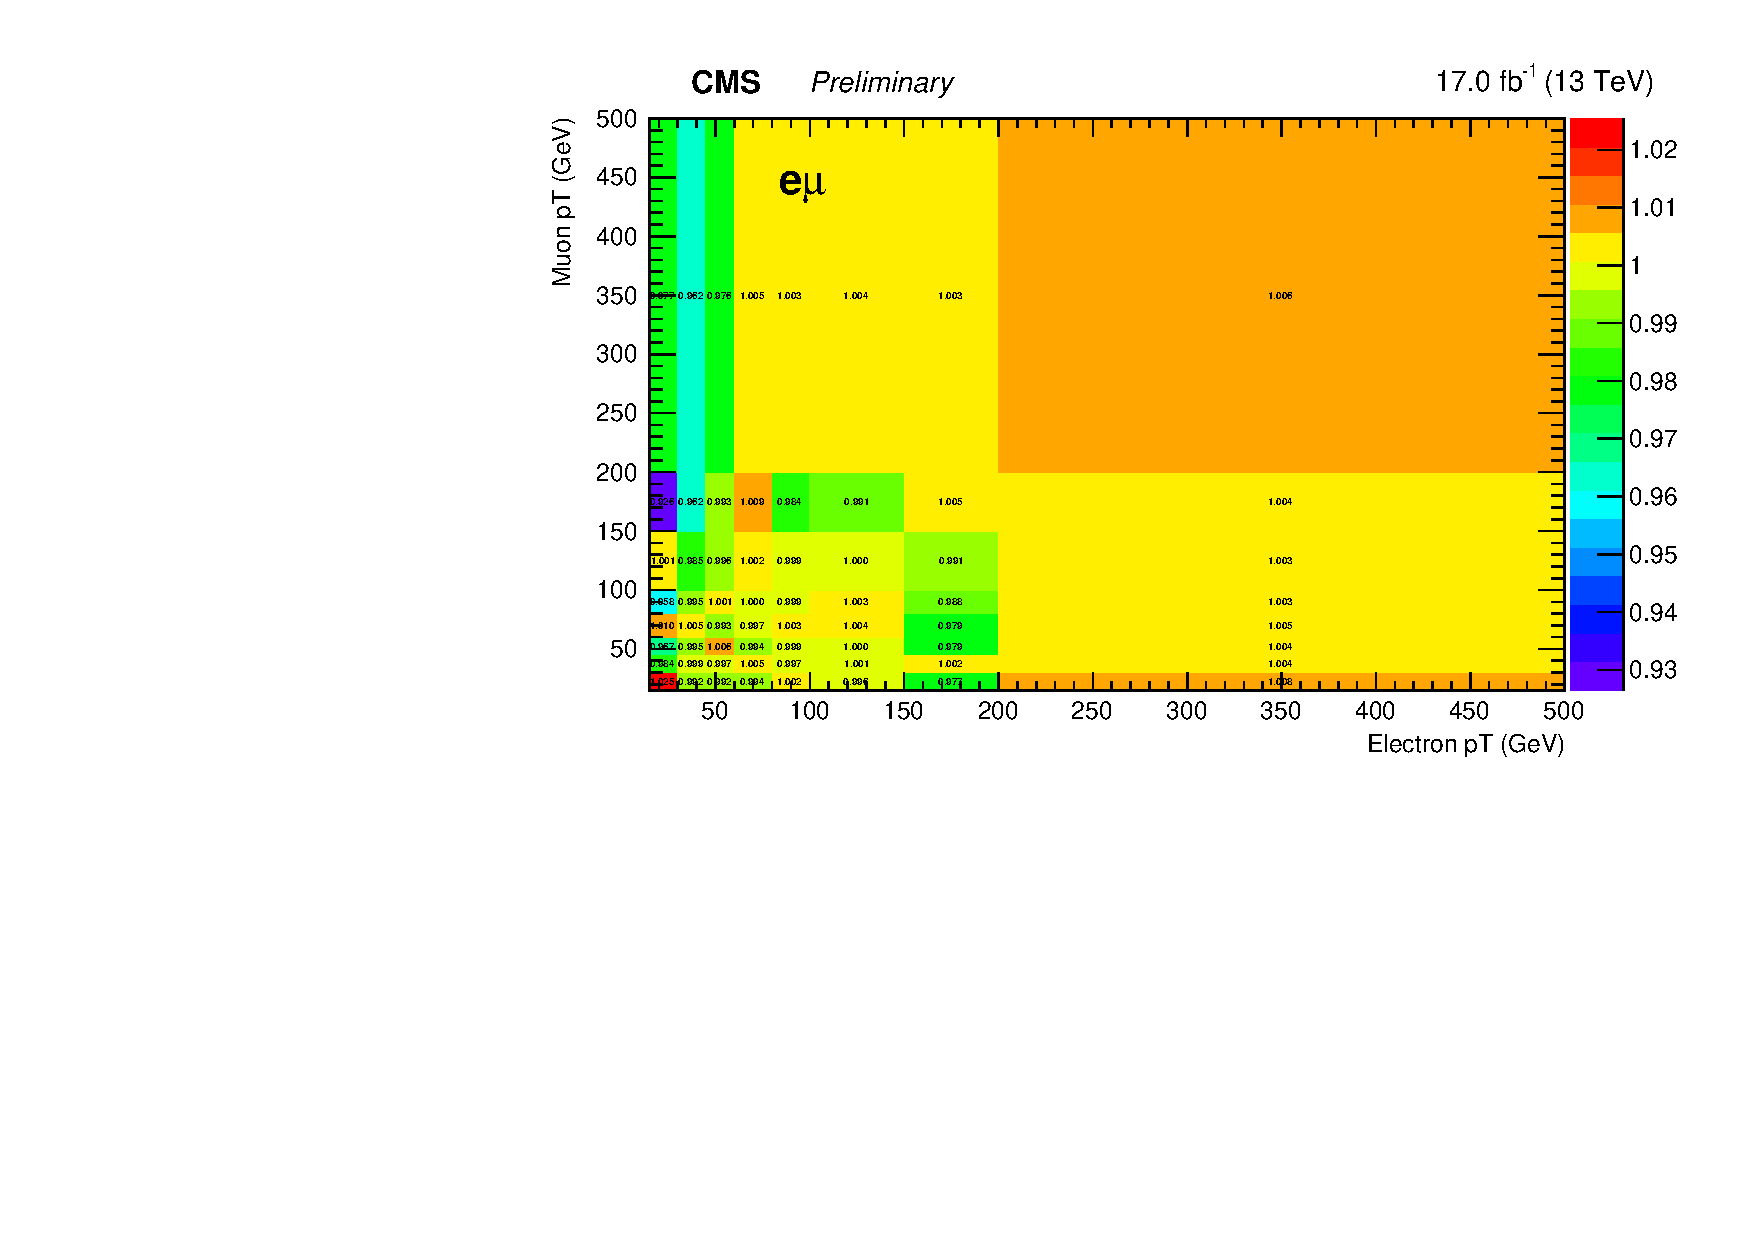
\includegraphics[width=0.50\textwidth]{fig_2016postVFP_TrigSF/h2D_lepABpt_emu.pdf}
      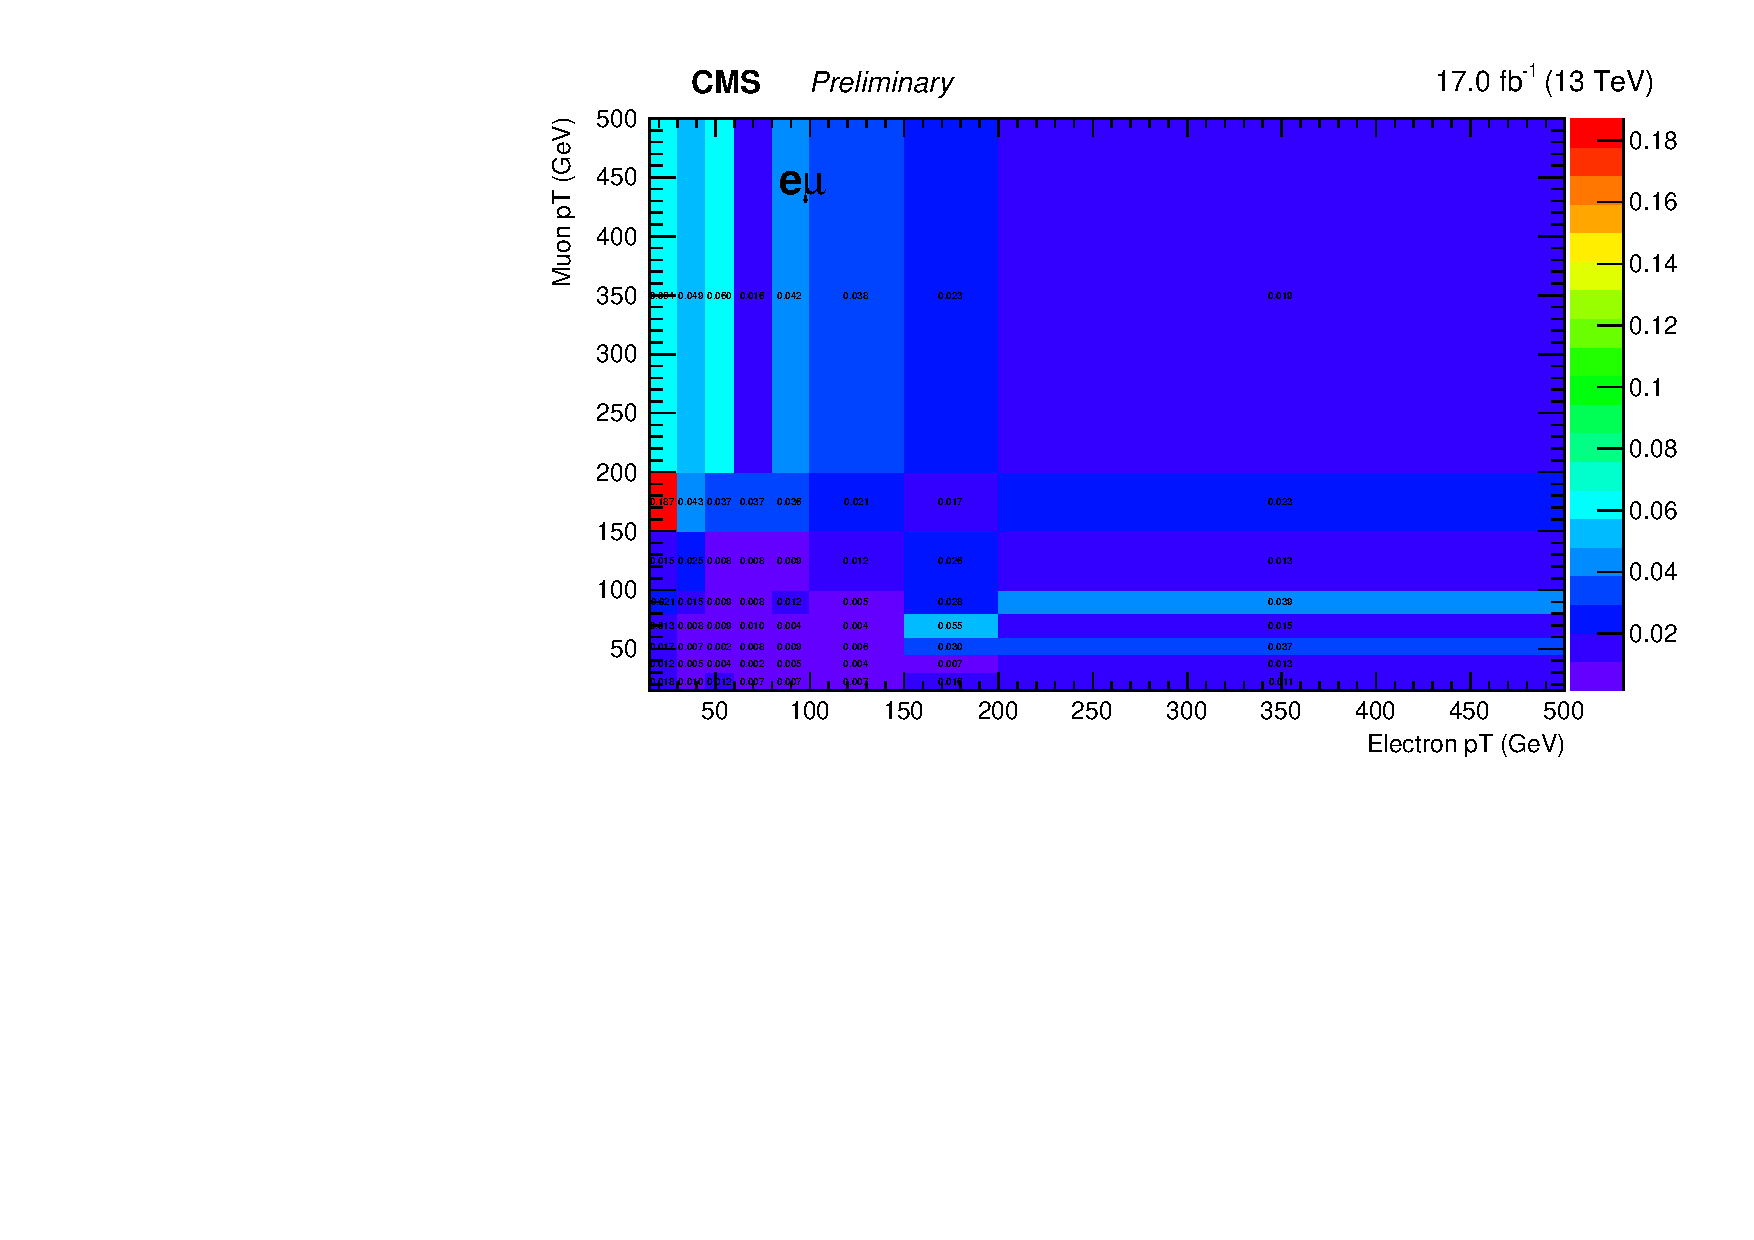
\includegraphics[width=0.50\textwidth]{fig_2016postVFP_TrigSF/h2D_lepABpt_emu_BinErrors.pdf}\\       
      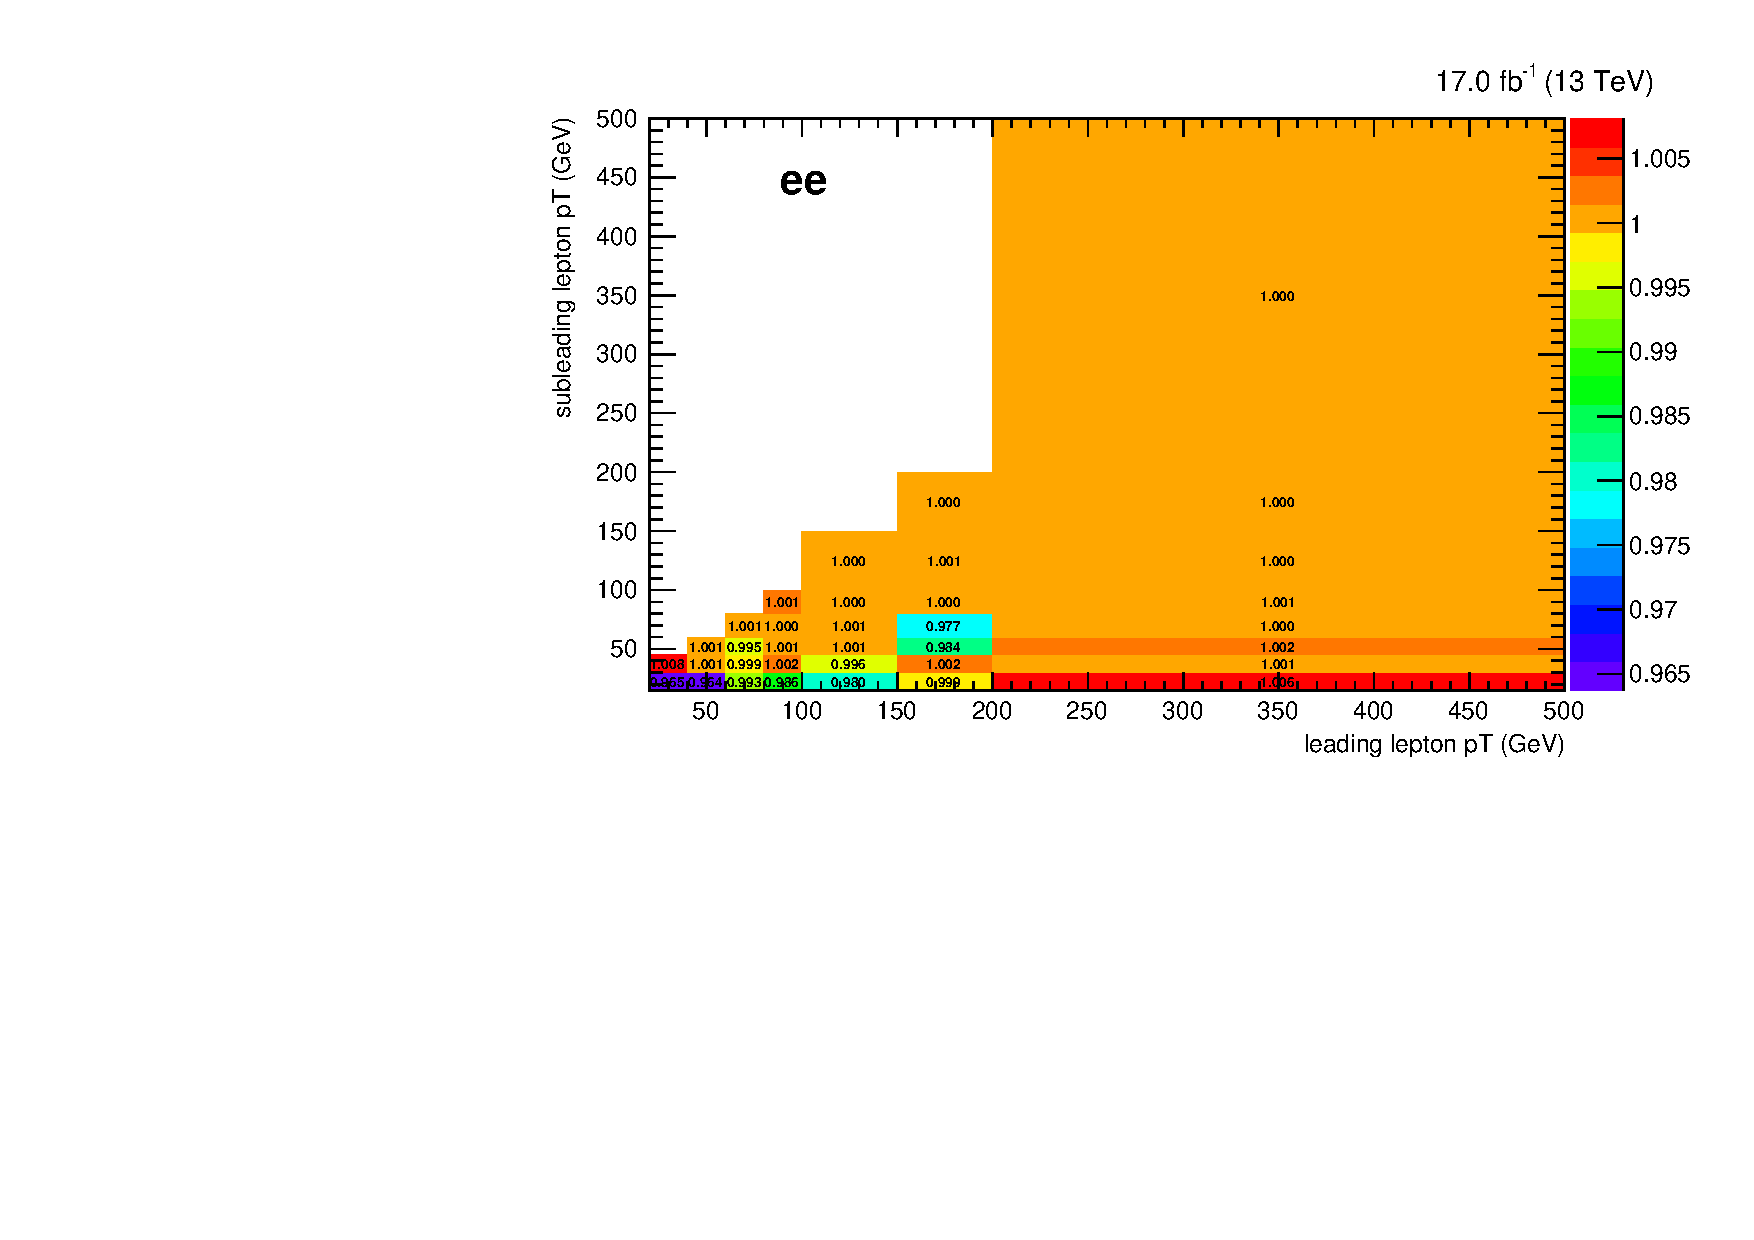
\includegraphics[width=0.50\textwidth]{fig_2016postVFP_TrigSF/h2D_lepABpt_ee.pdf}
      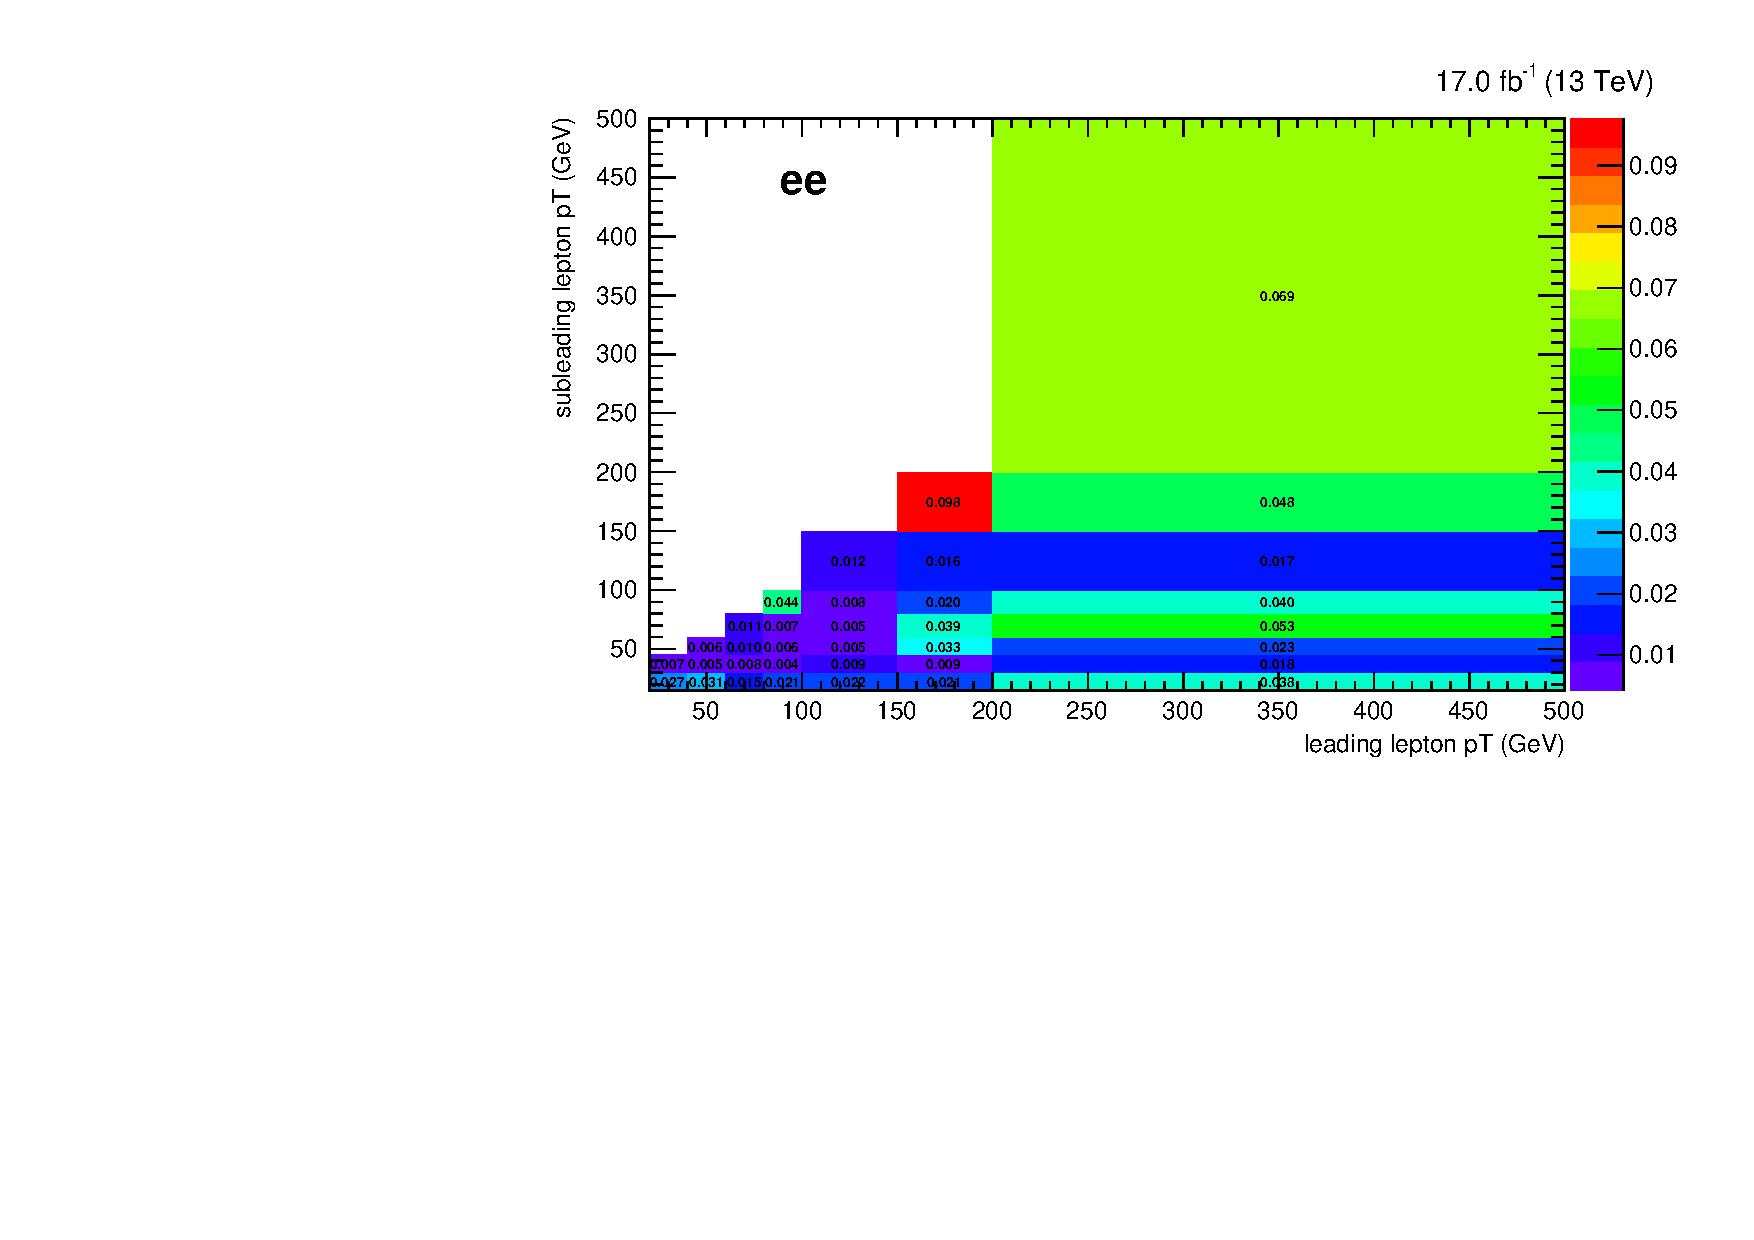
\includegraphics[width=0.50\textwidth]{fig_2016postVFP_TrigSF/h2D_lepABpt_ee_BinErrors.pdf}\\
      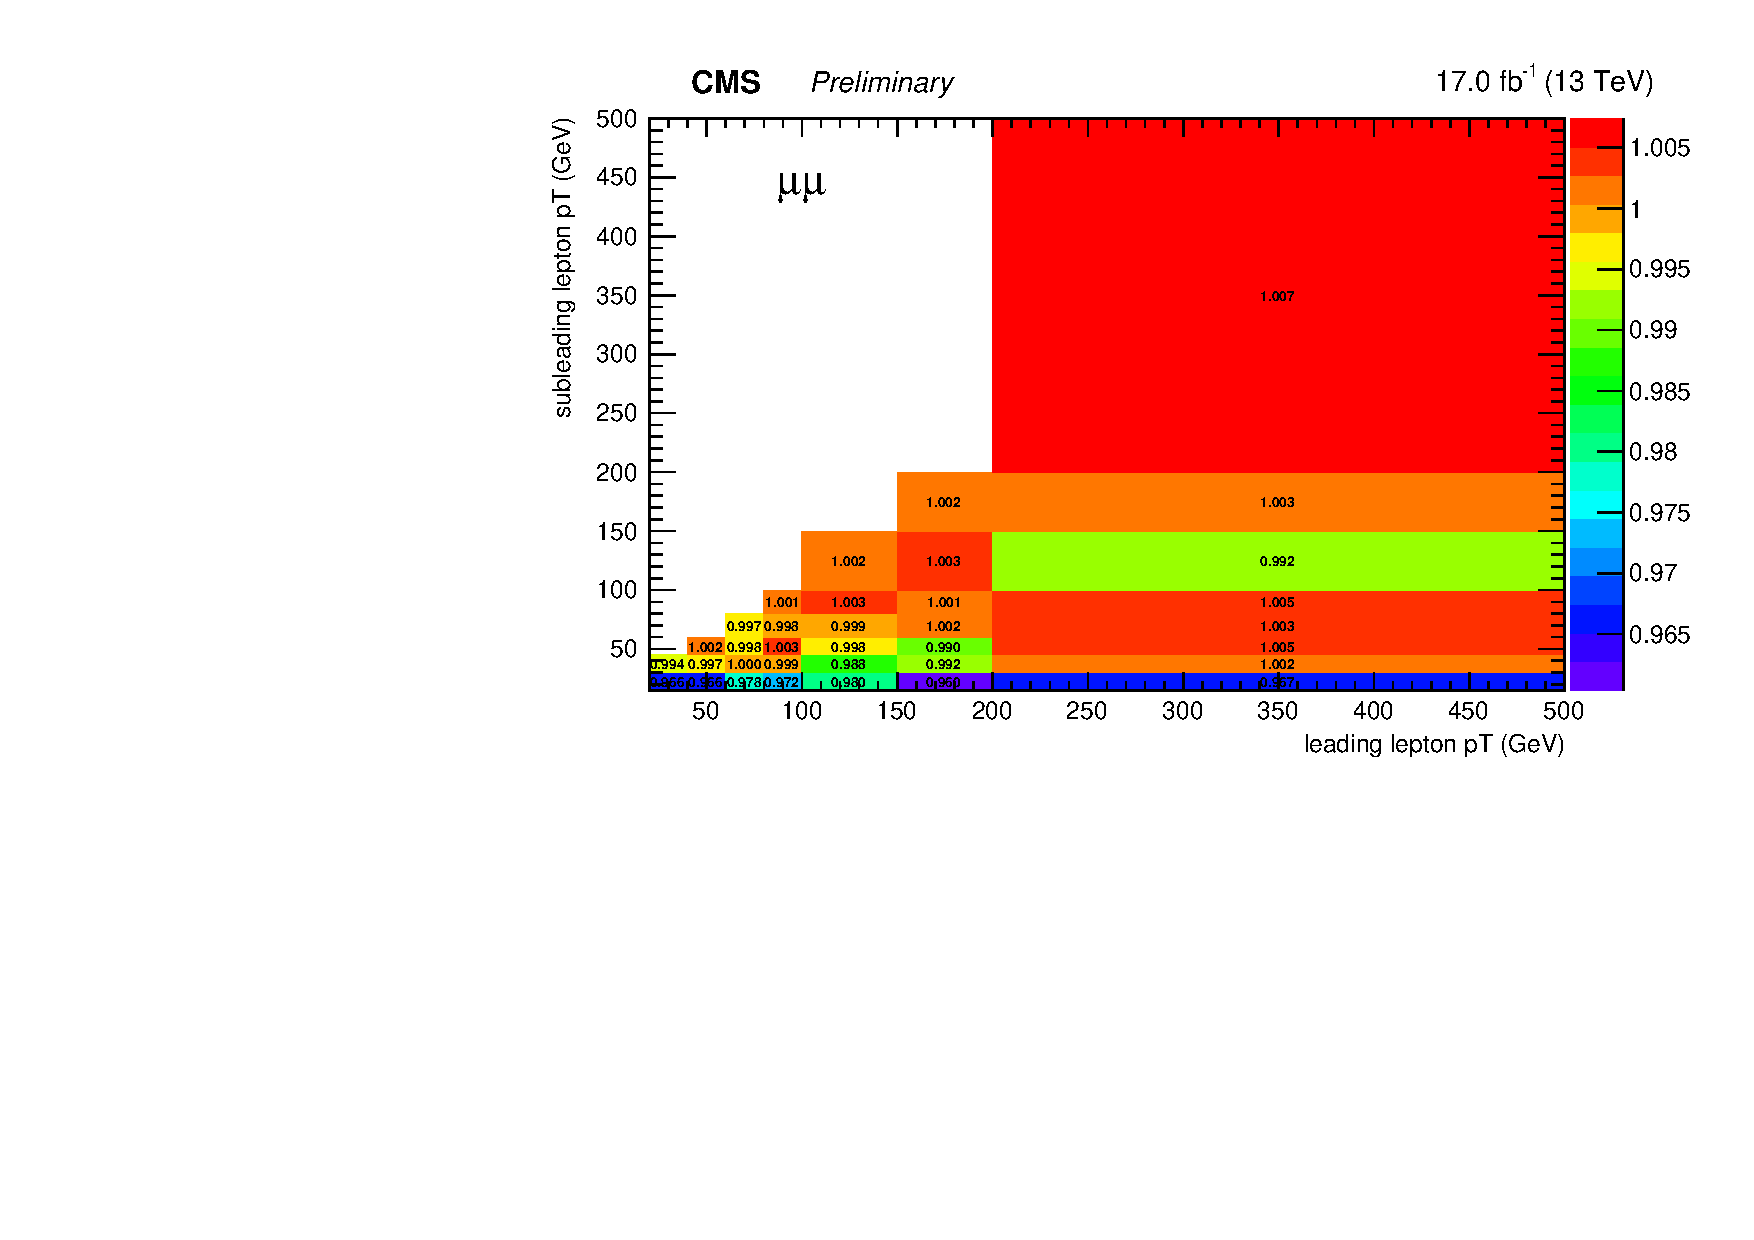
\includegraphics[width=0.50\textwidth]{fig_2016postVFP_TrigSF/h2D_lepABpt_mumu.pdf}
      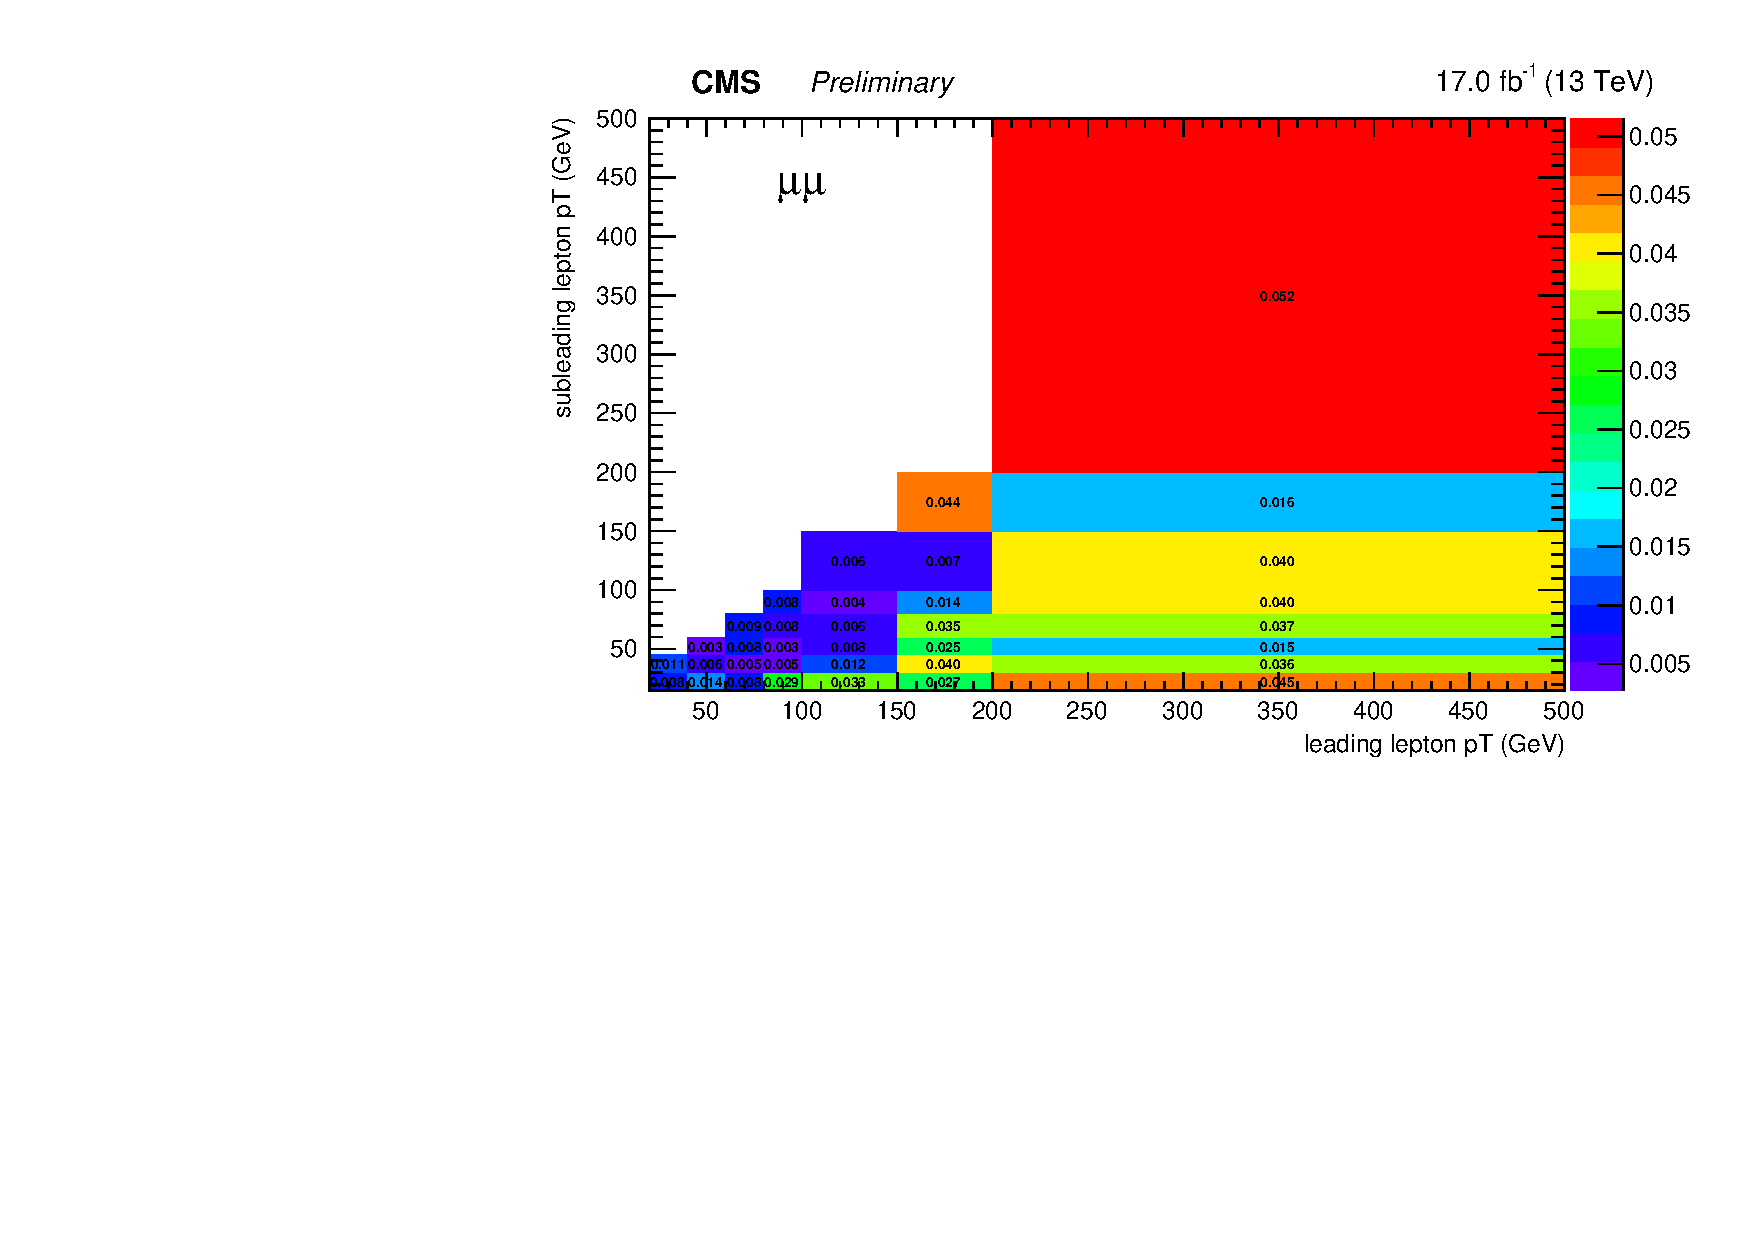
\includegraphics[width=0.50\textwidth]{fig_2016postVFP_TrigSF/h2D_lepABpt_mumu_BinErrors.pdf}\\
    \end{tabular}
    \caption{2D scale factors (Left) and total uncertainties (Right) for the 2016postVFP data set in the $e\mu$ (top), $ee$ (middle) and $\mu\mu$ (bottom) channels as a function of leading lepton \pT and sub-leading lepton \pT.}
    \label{TrigSF_2016postVFP_4}
  \end{center}
\end{figure}

\clearpage
\subsection{Trigger Efficiencies and Scale Factors: 2017}
\label{TrigSFResults2017}

\begin{figure}[h]
  \begin{center}
    \begin{tabular}{ccc}
      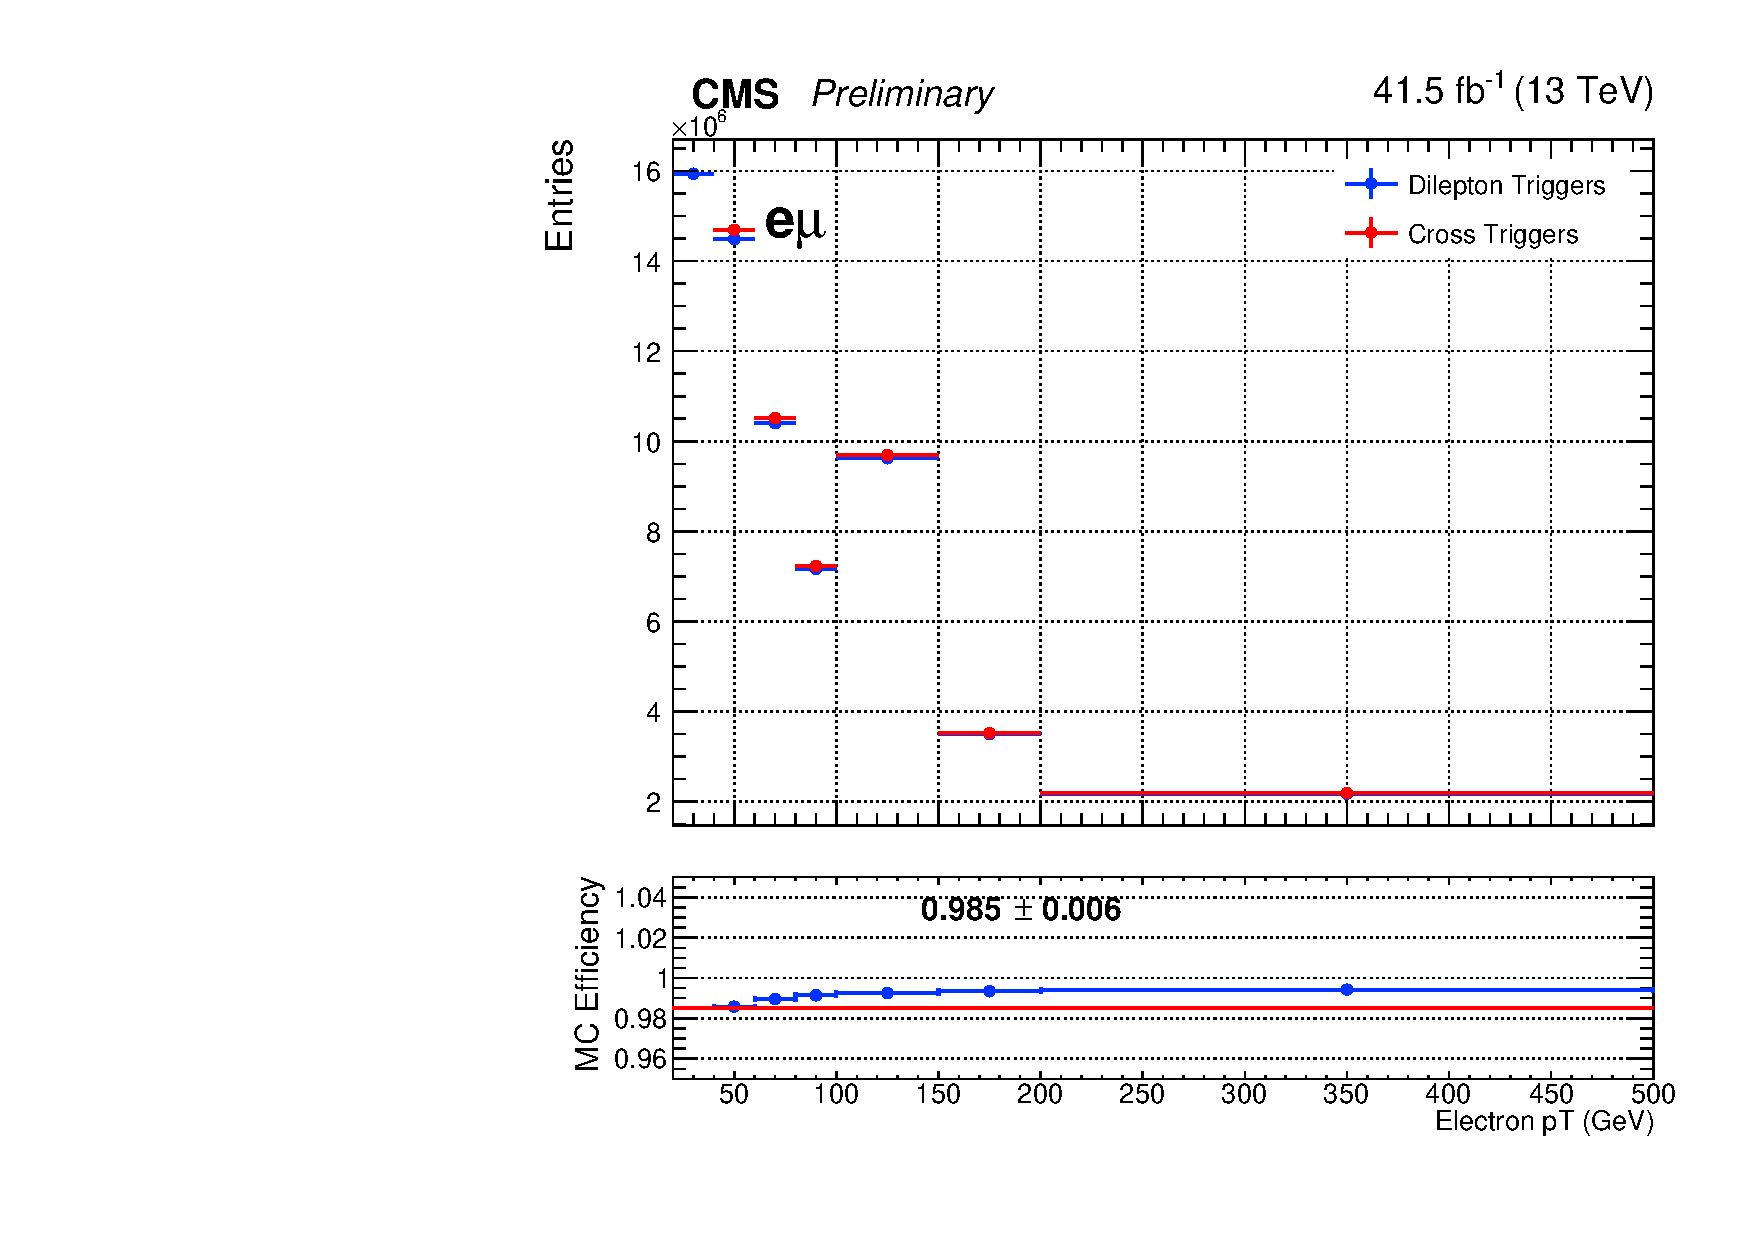
\includegraphics[width=0.32\textwidth]{fig_2017_TrigSF/g_lepApt_emu_MC.pdf}
      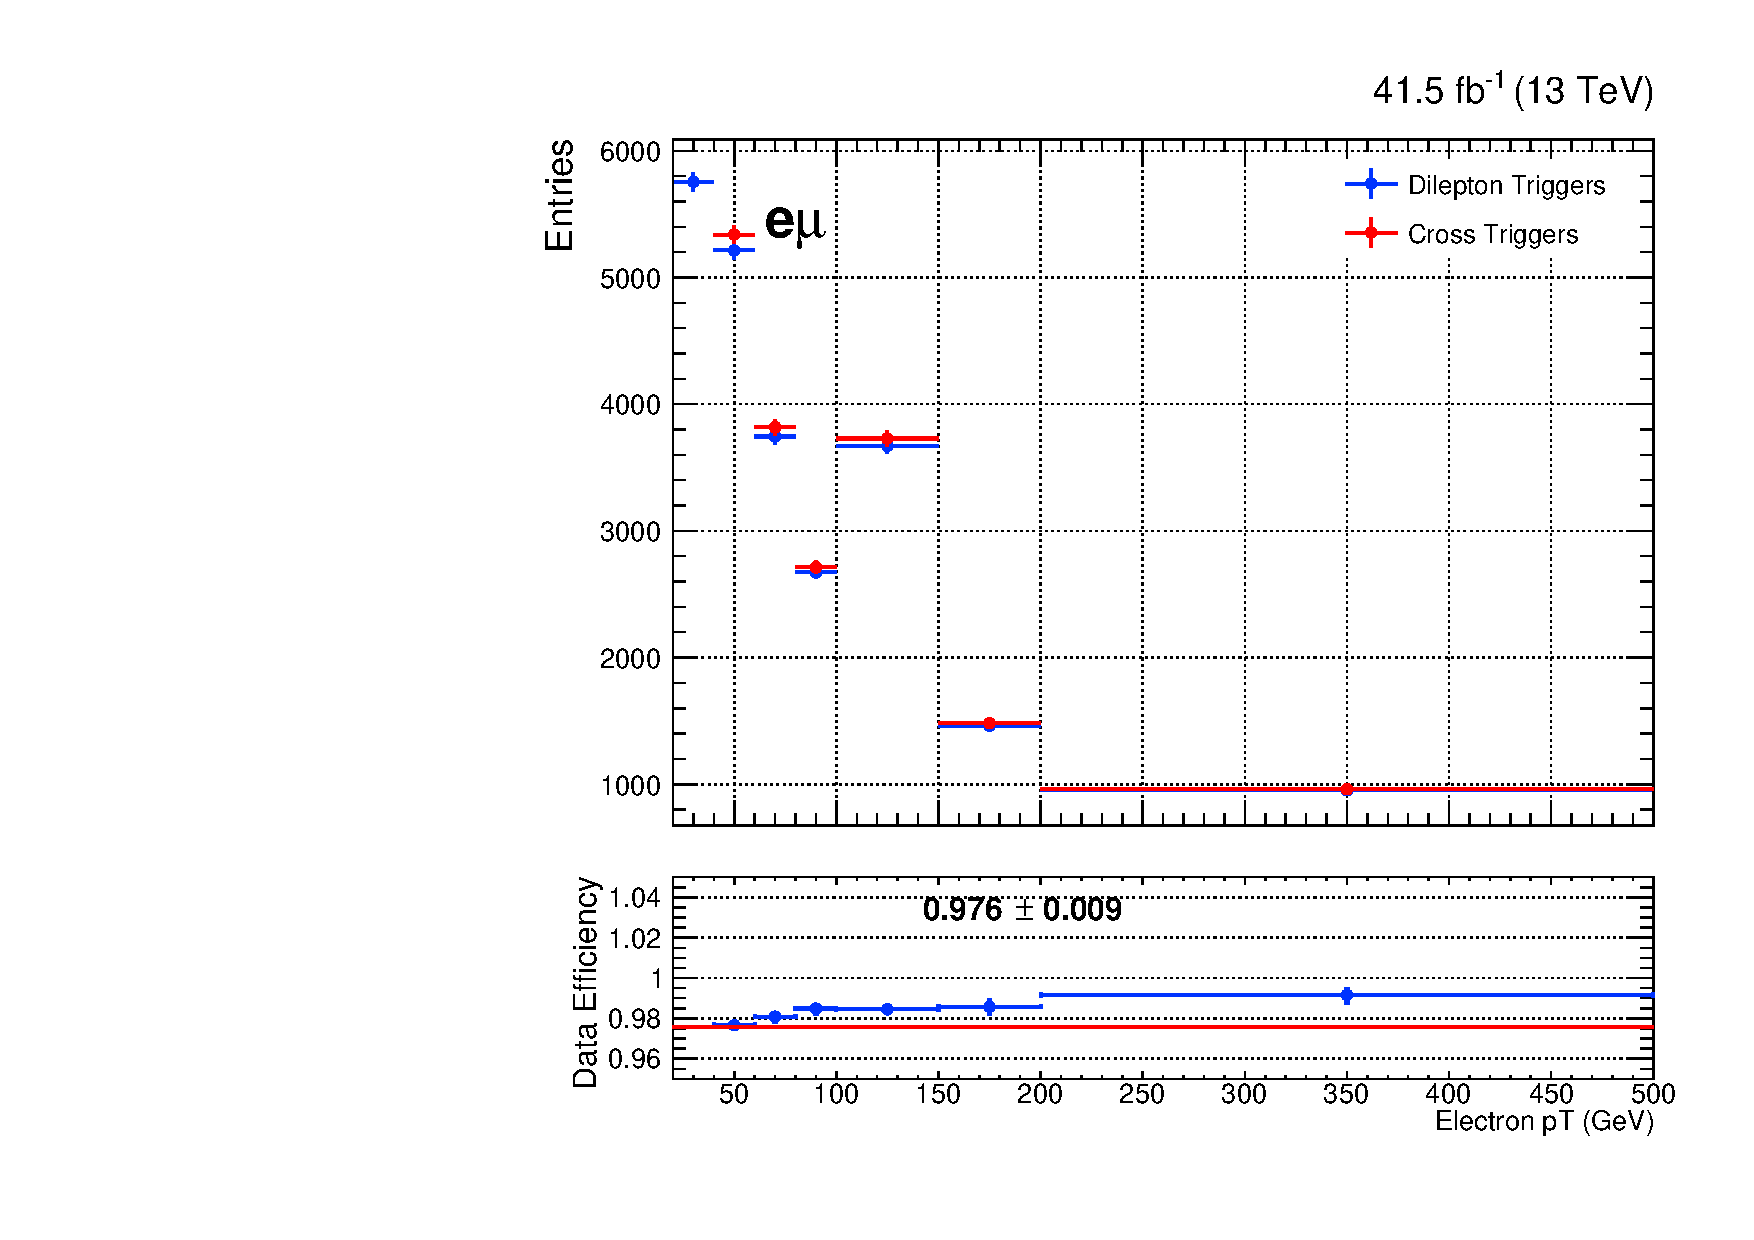
\includegraphics[width=0.32\textwidth]{fig_2017_TrigSF/g_lepApt_emu_data.pdf}
      \includegraphics[width=0.32\textwidth]{fig_2017_TrigSF/g_emu_lepApt_FullSystUncBand.pdf}\\
      \includegraphics[width=0.32\textwidth]{fig_2017_TrigSF/g_lepBpt_emu_MC.pdf}
      \includegraphics[width=0.32\textwidth]{fig_2017_TrigSF/g_lepBpt_emu_data.pdf}
      \includegraphics[width=0.32\textwidth]{fig_2017_TrigSF/g_emu_lepBpt_FullSystUncBand.pdf}\\
    \end{tabular}
    \caption{Efficiencies and scale factors for the 2017 data set in the $e\mu$ channel as a function of electron and muon \pT.
            The error bars indicate the statistical uncertainty, and the shaded band corresponds to the systematic uncertainty.
            }
    \label{TrigSF_2017_1}
  \end{center}
\end{figure}

\begin{figure}[h]
  \begin{center}
    \begin{tabular}{ccc}
      \includegraphics[width=0.32\textwidth]{fig_2017_TrigSF/g_lepApt_ee_MC.pdf}
      \includegraphics[width=0.32\textwidth]{fig_2017_TrigSF/g_lepApt_ee_data.pdf}
      \includegraphics[width=0.32\textwidth]{fig_2017_TrigSF/g_ee_lepApt_FullSystUncBand.pdf}\\
      \includegraphics[width=0.32\textwidth]{fig_2017_TrigSF/g_lepBpt_ee_MC.pdf}
      \includegraphics[width=0.32\textwidth]{fig_2017_TrigSF/g_lepBpt_ee_data.pdf}
      \includegraphics[width=0.32\textwidth]{fig_2017_TrigSF/g_ee_lepBpt_FullSystUncBand.pdf}\\
    \end{tabular}
    \caption{Efficiencies and scale factors for the 2017 data set in the $ee$ channel as a function of leading and sub-leading lepton \pT.
            The error bars indicate the statistical uncertainty, and the shaded band corresponds to the systematic uncertainty.
            }
    \label{TrigSF_2017_2}
  \end{center}
\end{figure}

\begin{figure}[h]
  \begin{center}
    \begin{tabular}{ccc}
      \includegraphics[width=0.32\textwidth]{fig_2017_TrigSF/g_lepApt_mumu_MC.pdf}
      \includegraphics[width=0.32\textwidth]{fig_2017_TrigSF/g_lepApt_mumu_data.pdf}
      \includegraphics[width=0.32\textwidth]{fig_2017_TrigSF/g_mumu_lepApt_FullSystUncBand.pdf}\\
      \includegraphics[width=0.32\textwidth]{fig_2017_TrigSF/g_lepBpt_mumu_MC.pdf}
      \includegraphics[width=0.32\textwidth]{fig_2017_TrigSF/g_lepBpt_mumu_data.pdf}
      \includegraphics[width=0.32\textwidth]{fig_2017_TrigSF/g_mumu_lepBpt_FullSystUncBand.pdf}\\
    \end{tabular}
    \caption{Efficiencies and scale factors for the 2017 data set in the $\mu\mu$ channel as a function of leading and sub-leading lepton \pT.
            The error bars indicate the statistical uncertainty, and the shaded band corresponds to the systematic uncertainty.
            }
    \label{TrigSF_2017_3}
  \end{center}
\end{figure}

\begin{figure}[h]
  \begin{center}
    \begin{tabular}{cc}
      \includegraphics[width=0.50\textwidth]{fig_2017_TrigSF/h2D_lepABpt_emu.pdf}
      \includegraphics[width=0.50\textwidth]{fig_2017_TrigSF/h2D_lepABpt_emu_BinErrors.pdf}\\       
      \includegraphics[width=0.50\textwidth]{fig_2017_TrigSF/h2D_lepABpt_ee.pdf}
      \includegraphics[width=0.50\textwidth]{fig_2017_TrigSF/h2D_lepABpt_ee_BinErrors.pdf}\\
      \includegraphics[width=0.50\textwidth]{fig_2017_TrigSF/h2D_lepABpt_mumu.pdf}
      \includegraphics[width=0.50\textwidth]{fig_2017_TrigSF/h2D_lepABpt_mumu_BinErrors.pdf}\\
    \end{tabular}
    \caption{2D scale factors (Left) and total uncertainties (Right) for the 2017 data set in the $e\mu$ (top), $ee$ (middle) and $\mu\mu$ (bottom) channels as a function of leading lepton \pT and sub-leading lepton \pT.}
    \label{TrigSF_2017_4}
  \end{center}
\end{figure}

\clearpage
\subsection{Trigger Efficiencies and Scale Factors: 2018}
\label{TrigSFResults2018}

\begin{figure}[h]
  \begin{center}
    \begin{tabular}{ccc}
      \includegraphics[width=0.32\textwidth]{fig_2018_TrigSF/g_lepApt_emu_MC.pdf}
      \includegraphics[width=0.32\textwidth]{fig_2018_TrigSF/g_lepApt_emu_data.pdf}
      \includegraphics[width=0.32\textwidth]{fig_2018_TrigSF/g_emu_lepApt_FullSystUncBand.pdf}\\
      \includegraphics[width=0.32\textwidth]{fig_2018_TrigSF/g_lepBpt_emu_MC.pdf}
      \includegraphics[width=0.32\textwidth]{fig_2018_TrigSF/g_lepBpt_emu_data.pdf}
      \includegraphics[width=0.32\textwidth]{fig_2018_TrigSF/g_emu_lepBpt_FullSystUncBand.pdf}\\
    \end{tabular}
    \caption{Efficiencies and scale factors for the 2018 data set in the $e\mu$ channel as a function of electron and muon \pT.
            The error bars indicate the statistical uncertainty, and the shaded band corresponds to the systematic uncertainty.
            }
    \label{TrigSF_2018_1}
  \end{center}
\end{figure}

\begin{figure}[h]
  \begin{center}
    \begin{tabular}{ccc}
      \includegraphics[width=0.32\textwidth]{fig_2018_TrigSF/g_lepApt_ee_MC.pdf}
      \includegraphics[width=0.32\textwidth]{fig_2018_TrigSF/g_lepApt_ee_data.pdf}
      \includegraphics[width=0.32\textwidth]{fig_2018_TrigSF/g_ee_lepApt_FullSystUncBand.pdf}\\
      \includegraphics[width=0.32\textwidth]{fig_2018_TrigSF/g_lepBpt_ee_MC.pdf}
      \includegraphics[width=0.32\textwidth]{fig_2018_TrigSF/g_lepBpt_ee_data.pdf}
      \includegraphics[width=0.32\textwidth]{fig_2018_TrigSF/g_ee_lepBpt_FullSystUncBand.pdf}\\
    \end{tabular}
    \caption{Efficiencies and scale factors for the 2018 data set in the $ee$ channel as a function of leading and sub-leading lepton \pT.
            The error bars indicate the statistical uncertainty, and the shaded band corresponds to the systematic uncertainty.
            }
    \label{TrigSF_2018_2}
  \end{center}
\end{figure}

\begin{figure}[h]
  \begin{center}
    \begin{tabular}{ccc}
      \includegraphics[width=0.32\textwidth]{fig_2018_TrigSF/g_lepApt_mumu_MC.pdf}
      \includegraphics[width=0.32\textwidth]{fig_2018_TrigSF/g_lepApt_mumu_data.pdf}
      \includegraphics[width=0.32\textwidth]{fig_2018_TrigSF/g_mumu_lepApt_FullSystUncBand.pdf}\\
      \includegraphics[width=0.32\textwidth]{fig_2018_TrigSF/g_lepBpt_mumu_MC.pdf}
      \includegraphics[width=0.32\textwidth]{fig_2018_TrigSF/g_lepBpt_mumu_data.pdf}
      \includegraphics[width=0.32\textwidth]{fig_2018_TrigSF/g_mumu_lepBpt_FullSystUncBand.pdf}\\
    \end{tabular}
    \caption{Efficiencies and scale factors for the 2018 data set in the $\mu\mu$ channel as a function of leading and sub-leading lepton \pT.
            The error bars indicate the statistical uncertainty, and the shaded band corresponds to the systematic uncertainty.
            }
    \label{TrigSF_2018_3}
  \end{center}
\end{figure}

\begin{figure}[h]
  \begin{center}
    \begin{tabular}{cc}
      \includegraphics[width=0.50\textwidth]{fig_2018_TrigSF/h2D_lepABpt_emu.pdf}
      \includegraphics[width=0.50\textwidth]{fig_2018_TrigSF/h2D_lepABpt_emu_BinErrors.pdf}\\       
      \includegraphics[width=0.50\textwidth]{fig_2018_TrigSF/h2D_lepABpt_ee.pdf}
      \includegraphics[width=0.50\textwidth]{fig_2018_TrigSF/h2D_lepABpt_ee_BinErrors.pdf}\\
      \includegraphics[width=0.50\textwidth]{fig_2018_TrigSF/h2D_lepABpt_mumu.pdf}
      \includegraphics[width=0.50\textwidth]{fig_2018_TrigSF/h2D_lepABpt_mumu_BinErrors.pdf}\\
    \end{tabular}
    \caption{2D scale factors (Left) and total uncertainties (Right) for the 2018 data set in the $e\mu$ (top), $ee$ (middle) and $\mu\mu$ (bottom) channels as a function of leading lepton \pT and sub-leading lepton \pT.}
    \label{TrigSF_2018_4}
  \end{center}
\end{figure}

\clearpage
\newpage
\section{Search for Lorentz Invariance Violation in \ttbar Production}
Lorentz symmetry, i.e. that the laws of physics are the same in all inertial frames of reference, is a fundamental principle of general relativity and relativistic quantum field theories.
The search for violation of Lorentz symmetry involves looking for deviations from this symmetry, which could indicate the presence of new physics BSM.
One method to test the validity of Lorentz symmetry is to search for a modulation of the \ttbar cross section as a function of sidereal time (the orientation of the experiment relative to the fixed position of stars in the sky).
In order to accommodate a search and provide time dependence, the dilepton trigger efficiency scale factors were measured 1-Dimensionally as a function of sidereal time using the same method outlined above, with the exception of not including the number of vertices partition as a source of event topology systematic uncertainty.
\subsection{Translating UNIX Time to Sidereal Time}
Every CMS data event is recorded with a UNIX timestamp. 
The sidereal day, which is the time it takes for one rotation of the Earth relative to the stars, is about four minutes shorter than the solar day, which is the time it takes for one rotation of the Earth relative to the Sun.
In UNIX time, the rotational period of the earth (sidereal day) lasts approximately 23h 56min 4s, i.e. 86164 UNIX seconds. 
The sidereal second is defined in such a way that the rotational period of the earth is exactly 24h, i.e. 86400 sidereal seconds.
The following formula is used to translate UNIX time to sidereal time:
\begin{equation}
\Omega_{sidereal} t_{sidereal} = \Omega_{UTC} \times (t_{UNIX} - t_0) + \phi_{UNIX} + \phi_{longitude}
\end{equation}
In this equation:
\begin{itemize}
\item $\Omega_{sidereal}$ is the angular velocity of earth's rotation around its axis in sidereal time: $\Omega_{sidereal} = 2\pi / 86400 s^{-1}$ (sidereal). 
\item On the other hand, $\Omega_{UTC}$ is the angular velocity of earth's rotation around its axis in UTC time: $\Omega_{UTC} = 2\pi / 86164 s^{-1}$ (UTC). 
\item The symbol $t_{UNIX}$ represents the event timestamp recorded at CMS, in UNIX time; this is the number of UTC seconds since the UNIX epoch, i.e. the 1st of January 1970. However, handling large number of seconds is sometimes not practical and a $t_0$ origin is subtracted to set the origin at the first second of 2016.
\item The azimuth angle $\phi_{UNIX}$ encodes the phase between the Unix epoch and "J2000", which is the origin of sidereal time count. J2000 is defined as the direction pointed by the crossing of ecliptic and equator plans, at noon the 1st of January 2000, on the side of the earth were the Sun moves from the Southern hemisphere to the Northern hemisphere. 
\item The azimuth $\phi_{longitude}$ is the effective longitude of the beam at CMS relative to the Greenwich meridian, in radians.
\end{itemize}

\clearpage
\newpage
\subsection{Time Dependent Trigger Scale Factors: 2016}
\label{TrigSFResults_SideReal_2016}

\begin{figure}[h]
  \begin{center}
    \begin{tabular}{cc}
      \includegraphics[width=0.32\textwidth]{fig_2016_sidereal/g_emu_sidereel_FullSystUncBand.pdf}
      \includegraphics[width=0.50\textwidth]{fig_2016_sidereal/g_emu_sidereel_ErrorsBreakdown.pdf}\\
    \end{tabular}
    \caption{Trigger scale factors for the 2016 data set in the $e\mu$ channel as a function of sidereal time.
            The error bars indicate the statistical uncertainty, and the shaded band corresponds to the systematic uncertainty.
            }
    \label{TrigSF_SideReal_2016_1}
  \end{center}
\end{figure}

\newpage
\subsection{Time Dependent Trigger Scale Factors: 2017}
\label{TrigSFResults_SideReal_2017}

\begin{figure}[h]
  \begin{center}
    \begin{tabular}{cc}
      \includegraphics[width=0.32\textwidth]{fig_2017_sidereal/g_emu_sidereal_FullSystUncBand.pdf}
      \includegraphics[width=0.50\textwidth]{fig_2017_sidereal/g_emu_sidereal_ErrorsBreakdown.pdf}\\
    \end{tabular}
    \caption{Trigger scale factors for the 2017 data set in the $e\mu$ channel as a function of sidereal time.
            The error bars indicate the statistical uncertainty, and the shaded band corresponds to the systematic uncertainty.
            }
    \label{TrigSF_SideReal_2017_1}
  \end{center}
\end{figure}